\documentclass[
	reqno, 
	fontsize=12pt, 
	twoside,
	numbers=noenddot	% Removes dots after figure labels (Figure 1.: ... becomes Figure 1: ...)
	]{scrbook}

\usepackage{arbeit}


%% Flags
\newtoggle{classneg}
\togglefalse{classneg}
\def\layouthack		#1{#1}

%% math-Abbreviations
\def\defeq			{\mathrel{\mathop:}=}
\def\eqdef			{=\mathrel{\mathop:}}
\def\defequiv		{\mathrel{\mathop:}\Leftrightarrow}
\def\pow			#1{{\mathcal{P}(#1)}}
\def\restrict		#1{{\big |_{#1}}}
\def\natural		{\mathbb{N}}
\def\field			{\mathbb{K}}
\def\ideal			{\mathfrak{a}}
\def\O				{\mathcal{O}}
\def\S				{\mathcal{S}}
\def\code			{\text{code}}
\def\acts			{{\ \circlearrowleft\ }}
\def\msix				{{$\overline{M}_{0,6}$}}

%%gpispace expressions
\def\gpigt			{\mathrel{\text{:gt:}}}
\def\gpiresolve		#1{{\$\{#1\}}}

%% text-Abbreviations
\def\singular		{\textsc{Singular}}
\def\libsingular	{\textsc{libSingular}}
\def\gitfanlib		{\textsc{gitfan.lib}}
\def\gpispace		{\textsc{GPI-Space}}
\def\beegfs			{\textsc{BeeGFS}}
\def\cplusplus		{\textsc{C++}}
\def\c				{\textsc{C}}
\def\gtest			{\textsc{Google Test}}
\def\aface			{$\ideal$\=/face}
\def\afaces			{$\ideal$\=/faces}

%% Define keywords for algorithms.
\SetKw{Not}{not}
\SetKw{Null}{null}
\SetKw{And}{and}
\SetKw{Or}{or}
\SetKw{New}{new}
\SetKw{True}{true}
\SetKw{Continue}{continue}
\SetKw{Break}{break}
\SetKwFunction{First}{first}
\SetKwComment{Comment}{/* }{ */}
\SetKwInput{KwDependencies}{Dependencies}
\SetKwData{Map}{Map}
\SetKwData{List}{List}
\SetKwData{Queue}{Queue}

%% Provide command for a raised chi so that it does not exceed the baseline
\DeclareRobustCommand{\rchi}{{\mathpalette\irchi\relax}}
\newcommand{\irchi}[2]{\raisebox{0.85\depth}{$#1\chi$}} % inner command, used by \rchi

%% Langer Trennstrich
\def\horizontalline	{\noindent\makebox[\linewidth]{\rule{\paperwidth}{0.4pt}}}

%% Unbreakable block
\AtBeginEnvironment{nobreak}{\begin{minipage}{\textwidth}}
\AtEndEnvironment{nobreak}{\end{minipage}}

%% Block für Einschübe
\definecolor{light-gray}{gray}{0.95}
\newcommand{\Block}[1]{
\vspace{2mm}\noindent
\fcolorbox{black}{light-gray}{ \begin{minipage}[r]{0.97\textwidth}
		\setcounter{mpfootnote}{\value{footnote}}
		\renewcommand{\thempfootnote}{\arabic{mpfootnote}}
		
		#1
		
		\setcounter{footnote}{\value{mpfootnote}}
	\end{minipage} }
}
\bibliography{references}

% Fix hypenation
\hyphenation{Fur-ther-more}
                                 
\begin{document}
	
	\newcommand{\TypeDerArbeit}{Masterarbeit}
	\newcommand{\Student}{Christian Reinbold}
	\newcommand{\Betreuer}{\parbox[t]{8cm}{apl. Prof. Dr. Anne Frühbis-Krüger \\ Dr. Janko Böhm \\ Dr. Mirko  Rahn}}
	\newcommand{\Kooperation}{Technische Universität Kaiserslautern \\
							  Fraunhofer-Institut für Techno- und Wirtschaftsmathematik}
	\newcommand{\Matrikelnummer}{2942360}
	\newcommand{\Erstpruefer}{apl. Prof. Dr. Anne Frühbis-Krüger}
	\newcommand{\Zweitpruefer}{Dr. Janko Böhm}
	\newcommand{\AbgabeDerArbeit}{11.01.2018}
	\newcommand{\TitelDerArbeit}{Computation of the GIT-fan using a massively parallel implementation}
	\newcommand{\Einrichtung}{Leibniz Universität Hannover\\Fakultät für Mathematik und Physik\\Institut für Algebraische Geometrie}
	
	\begin{titlepage}
	\begin{center}
		\vfill
		
		\begin{minipage}[t]{0.47\textwidth}
			
\includegraphics[width=\textwidth]{logo.png}
		\end{minipage}
		\\[.5cm]
		\Large \Einrichtung \\[.5cm]
		
		\large in Kooperation mit \\ \Large \Kooperation \\[1cm]
		
		{\color{blue}\hrule height 1.1pt}~\\ 
		{\LARGE \textbf{\TitelDerArbeit}}\\[.4cm]
		{\color{blue}\hrule height 1.1pt}~\\
		
		\large \TypeDerArbeit		
		
		\vspace{1cm}
		\large Hannover, \AbgabeDerArbeit
		
		\large \Student
		
		\large Matrikelnr.: \Matrikelnummer
		
		\vfill
		
		\begin{tabular}{p{3cm}l}
			Erstprüfer:		& \Erstpruefer \\
			Zweitprüfer:	& \Zweitpruefer \\ 
			& \\
			Betreuer:		& \Betreuer
		\end{tabular}
	\end{center}
	
\end{titlepage}
	
	\frontmatter
	{
		\pagestyle{plain}
		\begin{center}
	\Large \textbf{Abstract}
\end{center}

The GIT fan of an algebraic group action on an algebraic variety describes all GIT quotients arising from Mumford's construction in Geometric Invariant Theory. In this thesis we enhance an implementation that computes the GIT fan for toric actions on affine varieties such that it may be executed on scalable hardware systems. For this purpose, we combine the parallelisation framework \gpispace{}, developed at the \acl{Fraunhofer ITWM}, and the computer algebra system \singular{}, developed at the \emph{Technische Universität Kaiserslautern}. In doing so, we are able to compute the Mori chamber decomposition of $\Mov(\overline{M}_{0,6})$ in approximately 21 minutes, utilising 40 \emph{Dell PowerEdge M620 Blade Servers} with 16 cores each.

%\cleardoublepage

\begin{center}
\Large \textbf{Kurzzusammenfassung}
\end{center}

Der GIT\=/Fächer einer algebraischen Gruppwirkung auf einer algebraischen Varietät beschreibt sämtliche GIT\=/Quotienten, die aus Mumfords Konstruktion im Bereich der geometrischen Invariantentheorie hervorgehen. In dieser Arbeit erweitern wir eine bereits bestehende Implementation zur Berechnung des GIT\=/Fächers für torische Gruppenwirkungen auf affinen Varietäten so, dass sie auf beliebig großen Rechnerverbunden parallel ausgeführt werden kann. Hierzu kombinieren wir das am \acl{Fraunhofer ITWM} entwickelte Parallelisierungsframework \gpispace{} mit dem Computeralgebrasystem \singular{} der \emph{Technischen Universität Kaiserslautern}. Mit der neuen Implementation können wir die Zerlegung von $\Mov(\overline{M}_{0,6})$ in seine Mori\=/Kammern in rund 21 Minuten berechnen. Verwendet werden hierbei 40 \emph{Dell PowerEdge M620 Blade Server} mit je 16 Kernen.
		\cleardoublepage
		\chapter*{Acknowledgements}
Syn, Ack...
	}
	\tableofcontents
	\cleardoublepage
	\mainmatter
	
	\addtolength{\headheight}{3pt}
	\setcounter{chapter}{0}
	\chapter{Introduction}

Algebraic group quotients are commonly used when constructing moduli spaces. A na\"{\i}ve moduli problem is a classification problem, that is a collection of objects together with an equivalence relation. Its moduli space setups a one\=/to\=/correspondence of its points and the equivalence classes. The projective line $\projective^1$ may be seen as a moduli space of the problem of classifying all nonzero points in the complex plane $\complex^2$ such that two points are equivalent iff they are contained in the same line through the origin. The elements of a class are generated by scaling points by a nonzero scalar. In other words, each class is an orbit of an action of the torus $\complex^*$ on the affine space $\complex^2$ without the origin. The moduli space $\projective^1$ is recovered by the orbit space. However, it is not equipped with a geometric structure by default. Thus, we obtain $\projective^1$ as a set but loose all geometric data attached to it as a projective variety. 

\ac{GIT} provides a method for creating algebraic group quotients with a geometric structure such that the quotient map becomes a morphism. In many instances the classical orbit space cannot be equipped with such a structure. Consider the complex plane $\complex^2$ with the torus action as above. Since the closure of each orbit -- that is a line -- contains the origin, every regular function being constant on orbits has to be constant on all $\complex^2$. On that account, the ring of regular functions of the orbit space would be the ground field $\complex$ and the orbit space would be a single point. Clearly, this is a contradiction. \ac{GIT} circumvents this problem by removing problematic orbits beforehand. The remaining ones form an open subset of \emph{semistable points} with a well behaving quotient that comes with a geometric structure. The quotient is \emph{almost geometric}, meaning that there exists a dense, open subset such that the quotient becomes the orbit space for this subset. In our case, we have to remove the origin from $\complex^2$ in order to obtain the orbit space $\projective^1$ together with its geometric description.

Mumford's construction of subsets of semistable points depends on a lifting of the group action to ample line bundles where different liftings may yield distinct subsets. There exists a quasifan, called \emph{GIT fan}, whose set of cones parametrises all subsets that may be obtained in this fashion. Given an affine variety together with a toric group action $H\acts X$, we focus on the computation of the GIT fan on scalable hardware systems. Basing on the work of \citeauthor{gitfan_symmetry} \cite{gitfan_symmetry}, we develop a cluster enabled application computing all chambers of the GIT fan of $H\acts X$. In doing so, we implement a fan traversal algorithm that is reusable in the context of tropical varieties \cite{tropical_varities} and Gröbner fans \cite[chapter 3]{sturmfels}.

The thesis is structured as follows: In the preliminaries, we cover the mathematical background encompassed by GIT fans. We introduce algebraic group actions and good categorical quotients, outline Mumford's construction of GIT quotients arising from subsets of semistable points and prove that the GIT cones associated to them indeed form a quasifan with convex support. The next chapter elucidates the algorithm we are going to implement. We describe how to express GIT cones in terms of orbit cones and compute the latter ones. Then, we translate the task of computing the GIT fan into a graph traversal problem and show how symmetries in the geometry of $X$ may be exploited in order to reduce the graph's size. Finally, we point out that \cite{gitfan_symmetry} incorporated an erroneous optimisation which we left out in our implementation. Fortunately, we were able to reproduce the results in \cite{gitfan_symmetry} without relying on the defect.

The fourth chapter covers the technical details of the cluster enabled implementation. Here, we introduce the utilised parallelisation framework \gpispace{} and follow up with the integration of \singular{} code into \gpispace{} applications. Furthermore, we present a high level description of our implementation in terms of Petri nets and document the various features of our application such as incorporating precomputed results. We finish off the chapter with a performance analysis for the computation of the Mori chamber decomposition of the cone of movable divisor classes of $\overline{M}_{0,6}$. The mathematical background of this example is outlined in the final chapter.

	\chapter{Preliminaries}

In this chapter we present the mathematical background used in the thesis. Step by step, we progress towards the construction and meaning of the GIT fan. The first section covers the notion of algebraic group actions which lead to various concepts of quotients introduced in the second section. Afterwards, we provide the details for constructing GIT quotients according to Mumford \cite{git}. Finally, a concrete description of available GIT quotients w.r.t.\ torus actions in terms of a quasifan is given. Computing this quasifan constitutes the main part of the thesis.

For the remainder of this chapter let $\field$ be an algebraically closed field.

%Gröbnerbasen, Buchberger

\section{Algebraic group actions}

In this section we extend the notion of groups acting on sets to actions on objects in algebraic geometry. We only cover the case of affine varieties here. For a more general approach considering pre\=/schemes, see \cite{git}. Broadly speaking, we require the group and the set operated on to carry structures of affine varieties such that the set\=/theoretical group action becomes a morphism.

\begin{defi}[Affine algebraic groups]
	An \emph{affine algebraic group} $G$ is an affine variety together with morphisms $m\colon G \times G \rightarrow G$ and $\iota\colon G \rightarrow G$ such that $G$ carries a group structure with the group law $m$ and inversion $\iota$. A \emph{homomorphism} of algebraic groups $G$ and $H$ is a morphism $f\colon G \rightarrow H$ such that $f$ preserves the group structure.
\end{defi}

\begin{ex}
	\label{example:algebraic_torus}
	The affine variety $$(\field^*)^n \cong V(t_1t_1^{-1} - 1,\dots, t_nt_n^{-1}-1)\subseteq\field[t_1,t_1^{-1},...,t_n,t_n^{-1}]$$
	is an affine algebraic group via the group law
	$$m\colon (\field^*)^n \times (\field^*)^n \rightarrow (\field^*)^n,\quad ((r_1,\dots,r_n),(s_1,\dots,s_n)) \mapsto (r_1s_1,\dots,r_ns_n)$$
	and the inversion
	$$\iota\colon(\field^*)^n \rightarrow (\field^*)^n,\quad (r_1,\dots,r_n) \mapsto (r_1^{-1},\dots,r_n^{-1}).$$
	Note that both $m$ and $\iota$ are polynomial when formulated over $\field[t_1,t_1^{-1},...,t_n,t_n^{-1}]$.
	
	We claim that the comultiplication $m^*$, that is the pullback of the multiplication $m$, is given by
	$$\O((\field^*)^n) \rightarrow \O((\field^*)^n) \tensor \O((\field^*)^n),\quad \mathbf{t}^\alpha \mapsto \mathbf{t}^\alpha \tensor \mathbf{t}^\alpha\quad \forall \alpha\in\integer^n.$$
	Clearly, this is a $\field$\=/algebra homormophism. It suffices to check equality with $m^*$ on a set of generators $\{\mathbf{t}^\alpha\mid \alpha\in\integer^n\}$. Now, 
	$$\mathbf{t}^\alpha \tensor \mathbf{t}^\alpha (P, Q) = P^\alpha\cdot Q^\alpha = (PQ)^\alpha =  (\mathbf{t}^\alpha \circ m) (P,Q) = m^*(\mathbf{t}^\alpha) (P,Q)$$ holds for all $\alpha\in\integer^n$ and $P,Q\in(\field^*)^n$. The claim follows.
\end{ex}

\begin{defi}
	An affine algebraic group $G$ is called \emph{(algebraic) torus of dimension $n$} iff there exists $n>0$ such that $G$ is isomorphic to the affine algebraic group $(\field^*)^n$.
\end{defi}

%\begin{remark}
%	\label{remark:torus_from_integral_vectors}
%	Let $\field$ be a algebraically closed field of characteristic zero. Then any finite set $\{v_1,\dots,v_r\}\subseteq\integer^k$ of integral vectors constitutes an algebraic torus of the same dimension as the linear subspace $L = \langle v_1,\dots,v_r\rangle_\rational$. Denote the dimension of $L$ by $d$. Then there exists an $\rational$-linear isomorphism such that $L\cong \rational^d$. In particular, this isomorphism translates to a $\field$\=/algebra isomorphism $\field[L] \cong \field[\rational^d]$ when $\rational$ is embedded into $\field$ as its prime field.
%	It follows that $\spec(\field[L])$ is an algebraic torus via
%	$$\spec(\field[L]) \cong \spec(\field[\rational^d]) =(\field^*)^d.$$
%\end{remark}

\begin{defi}[Algebraic Group action]
	Let $G$ be an affine algebraic group and $X$ be an affine variety. An (algebraic) group action of $G$ on $X$, denoted by $G\acts X$, is a morphism $\varphi\colon G\times X \rightarrow X$ such that $\varphi$ defines a set\=/theoretic group action of $G$ on $X$ via
	$$g\cdot x \defeq \varphi(g,x).$$
\end{defi}

%\begin{ex}
%	\label{example:torus_group_action}
%	Let $X = V(\ideal)\subseteq\field[x_1,\dots,x_r]$ be an affine variety such that its coordinate ring permits a $\integer^k$\=/grading. This grading extends to a $\integer^k$\=/grading of $\field[\mathbf{x}]$  via
%	$$\deg(x_i) \defeq \deg(\overline{x_i})\quad 1\leq i \leq r$$
%	so that $\ideal$ becomes homogeneous. The map
%	$$*\colon(\field^*)^k \times X \rightarrow X,\quad (t,P) \mapsto (t^{q_1}P_1,\dots,t^{q_r}P_r)$$
%	defines a group action. Clearly, the function is polynomial and the identity and compatibility axioms hold. It remains to check that it is well defined. Since we have $f(t*P) = t^q f(P)$ for all homogeneous polynomials $f$ of degree $q\in\integer^k$, for any point $P$ vanishing on the homogeneous ideal $\ideal$, $t*P$ also vanishes on $\ideal$.
%\end{ex}

\begin{construction}
	\label{construction:algebraic_torus}
	We give a concrete description of an algebraic torus $T$ of dimension $n$ acting on an affine variety $X$ via a morphism $\varphi\colon T\times X \rightarrow X$. It will turn out that group actions of $n$\=/dimensional tori on $X$ correspond to $\integer^n$\=/gradings on $\O(X)$.
	
	W.l.o.g. assume that $T = (\field^*)^n$ with the group law $m$ as specified in Example~\ref{example:algebraic_torus}. Note that the regular functions of $T$ are given by $\field[\mathbf{t},\mathbf{t}^{-1}]$ and the comultiplication $\varphi^*$ is injective since any regular function of $X$ vanishing on $TX$ also vanishes on $X$ by the identity axiom. Furthermore, we have $$\O(T)\tensor\O(T)\tensor\O(X)\cong\O(X)[\mathbf{t},\mathbf{t}^{-1},\mathbf{u},\mathbf{u}^{-1}]\quad\text{via}\quad\mathbf{t}^\alpha \tensor \mathbf{t}^\beta \tensor f \mapsto f\mathbf{t}^\alpha\mathbf{u}^\beta.$$
	For $\alpha\in\integer^n$, define
	$$\O(X)_\alpha \defeq \{f\in\O(X)\mid \varphi^*(f) = \mathbf{t}^\alpha \tensor f\},$$
	which is a submodule of $\O(X)$. Let $\sum_{\alpha\in I} f_\alpha$ be a finite linear combination of zero with $f_\alpha\in\O(X)_\alpha$. It follows that
	$$0 = \varphi^*(0) = \varphi^*\left(\sum_{\alpha\in I} f_\alpha\right) = \sum_{\alpha\in I} \varphi^*(f_\alpha) = \sum_{\alpha\in I} \mathbf{t}^\alpha \tensor f_\alpha.$$
	Coefficient comparison in $\O(X)[\mathbf{t},\mathbf{t}^{-1},\mathbf{u},\mathbf{u}^{-1}]$ shows that $f_\alpha = 0$. Hence, the sum
	$$\bigoplus_{\alpha\in\integer^n} \O(X)_\alpha \subseteqq \O(X)$$
	is direct.

	Let $f\in \O(X)$ and write $\varphi^*(f)$ as a finite linear combination
	$$\varphi^*(f) = \sum_{\alpha\in I} \mathbf{t}^\alpha \tensor f_\alpha.$$
	When moving to $\field$\=/algebra homomorphisms, the compatibility axiom translates to
	$$(m^* \tensor \id_{\O(X)}) \circ \varphi^* = (\id_{\O(T)} \tensor \varphi^*) \circ \varphi^*.$$
	Hence, we obtain
	$$\sum_{\alpha\in I} \mathbf{t}^\alpha \tensor \mathbf{t}^\alpha \tensor f_\alpha = (m^* \tensor \id_{\O(X)}) \circ \varphi^*(f) =  (\id_{\O(T)} \tensor \varphi^*) \circ \varphi^*(f) = \sum_{\alpha\in I}\mathbf{t}^\alpha \tensor \varphi^*(f_\alpha).$$
	Comparing coefficients yields $\varphi^*(f_\alpha) = \mathbf{t}^\alpha \otimes f_\alpha$, that is $f_\alpha\in \O(X)_\alpha$. Furthermore,
	$$\varphi^*\left(\sum_{\alpha\in I} f_\alpha\right) = \sum_{\alpha\in I} \varphi^*(f_\alpha) = \sum_{\alpha\in I} \mathbf{t}^\alpha \tensor f_\alpha = \varphi^*(f).$$
	$\varphi^*$ being injective implies that
	$$f = \sum_{\alpha\in I} f_\alpha,$$
	proving that
	$$\bigoplus_{\alpha\in\integer^n} \O(X)_\alpha = \O(X).$$
	Since $\varphi^*$ preserves the multiplication of $\O(X)$, it holds that $\O(X)_\alpha \O(X)_\beta \subseteq \O(X)_{\alpha+\beta}$. Hence, $\O(X)$ becomes a $\integer^n$\=/graded $\field$\=/algebra. Conversely, every $\integer^n$\=/grading on $\O(X)$ determines a group action $\psi$ of $T$ on $X$ with the corresponding coaction defined by 
	$$\psi^*(f) = \mathbf{t}^{\deg(f)}\tensor f\quad \forall f\in\O(X)\ \mathrm{homogeneous}.$$
	
	By taking a finite set $\{g_1,\dots,g_m\}$ of $\integer^n$\=/homogeneous generators of $\O(X)$, we obtain an embedding $X\subseteq\field^m$ such that the vanishing ideal $\ideal \defeq I(X)\subseteq\field[x_1,\dots,x_m]$ of $X$ is homogeneous w.r.t. the grading
	$$\deg(x_i) = \deg(g_i)\in\integer^n$$
	on $\field[x_1,\dots,x_m]$.
	By construction, we have $\varphi^*(g_i) = \mathbf{t}^{\deg(g_i)} \tensor g_i$ which translates to the coaction  $\psi^*(x_i) = \mathbf{t}^{\deg(g_i)} \tensor x_i$ in $\field[x_1,\dots,x_m] / \ideal$.
	The group action is recovered as follows:
	$$T \times X \longrightarrow X,\quad (t,P) \mapsto (\psi^*(x_1)(t,P),\dots,\psi^*(x_m)(t,P)) = (t^{\deg(g_1)}P_1,\dots,t^{\deg(g_m)}P_m).$$
	
	We conclude that any action of a torus of dimension $n$ on an affine variety $X$ may be described by a set of integral vectors $q_i\in\integer^n$, $1\leq i \leq m$, and a suitable embedding of $X$ in $\field^m$ such that its vanishing ideal is homogeneous w.r.t.
	$$\deg(x_i) = q_i,\quad 1\leq i \leq m.$$
	The group action is given by
	$$(\field^*)^n \times X \longrightarrow X,\quad (t,P) \mapsto (t^{q_1}P_1,\dots,t^{q_m}P_m).$$
\end{construction}

\begin{remark}
	Let $G$ be an affine algebraic group acting on an affine variety $X$. Let $x\in X$. The stabiliser subgroup $G_x$ is a closed, affine subvariety since it is the preimage of the closed point $\{x\}$ of the morphism $g\mapsto gx$. It follows that $G_x$ is an affine algebraic subgroup.
\end{remark}

\begin{remark}[Group action on regular functions]
	If $\varphi$ is a group action of an affine algebraic group $G$ on an affine variety $X$, we obtain a group action of $G$ on the regular functions $K(X)$ of $X$ by
	$$G\times K(X)\rightarrow K(X), \quad(g,\frac{f}{h}) \mapsto \frac{f\circ \varphi(g^{-1},\wildcard)}{h\circ \varphi(g^{-1},\wildcard)}\ .$$
	
	If $U$ is a $G$\=/invariant open subset of $X$, that is $GU = U$, the restriction of $G\acts K(X)$ to $\O_X(U)$ yields a group action $G\acts\O_X(U)$. Note that if the denominator $h$ does not vanish on any point in $U$, then the same holds for $h\circ \varphi(g^{-1},\wildcard)$ as we have $$\varphi(g^{-1},\wildcard)(U) \subseteq GU = U.$$
	
	We say that $f\in\O_X(U)$ is \emph{$G$\=/invariant} iff $gf = f$ holds for all $g\in G$. The subalgebra of $G$\=/invariant functions is denoted by $\O_X(U)^G$.
	\index{OXUG@$\O_X(U)^G$}%
\end{remark}

\begin{ex}
	\label{example:regular_functions_torus_group_action}
	Consider an algebraic group action $\varphi\colon T \times X \rightarrow X$ of a torus $T$ of dimension $n$ on an affine variety $X$. By Construction~\ref{construction:algebraic_torus}, $\O(X)$ is a $\integer^n$\=/graded $\field$\=/algebra. For any homogeneous $f\in\O(X)$ and $g\in (\field^*)^n$, we have
	$$(g^{-1}f)(x) = f \circ \varphi(g,x) = \varphi^*(f)(g,x) = (\mathbf{t}^{\deg(f)} \tensor f)(g,x) = g^{\deg(f)}\cdot f(x)\quad \forall x\in X.$$
	In particular, it is easy to see that
	$$g^{-1}f = g^\alpha f\quad \forall g\in (\field^*)^n \ \Longleftrightarrow \ f\in\O(X)_\alpha,$$
	where $\alpha\in\integer^n$, the left multiplication is given by the group action and the right one is the scalar multiplication of $\O(X)$ as $\field$\=/module.
	For this reason it follows that
	$$ \O(X)^T = \O(X)_0.$$
\end{ex}

\section{Good quotients}
When an algebraic group $G$ acts on an affine variety $X$, naturally one questions if the orbit space $X/G$ defined by the group action can be equipped with the structure of an variety such that the quotient map $p\colon X\rightarrow X/G$ becomes a morphism. Consider the following example.

\begin{ex}
	\label{example:bad_quotient}
	Let $G=\complex^*$ be a one dimensional algebraic torus action on the affine variety $X = \complex^2$ via scaling, that is
	$$(t,(x_1,x_2)) \mapsto (tx_1,tx_2).$$
	Each line $l$ through the origin in $\complex^2$ yields an orbit when removing 0. The origin is $G$\=/invariant and thus an orbit on its own.
	If the set\=/theoretical quotient map $p$ would be a morphism, a regular function $\varphi$ in $\O(X/G)$ induces a regular function $\psi = \varphi \circ p$ in $\O(X)$ that is $G$\=/invariant. In particular, $\psi$ has to be constant on the closure of each orbit. Since each closure contains the origin, $\psi$ and thus $\varphi$ have to be constant. It follows that $\O(X/G) \cong \field$, contradicting $|X/G| > 1$. Consequently, the set\=/theoretical quotient map is no good quotient in the following sense.
\end{ex}

\begin{defi}[Good quotient, \phantom{}{\cite[Definition 5.0.5]{cls}}]
	Let $G$ be an affine algebraic group acting on an affine variety $X$. A $G$\=/invariant morphism $p\colon X \rightarrow Y$ is called a \emph{good (categorial) quotient}, if
	\begin{enumerate}[label={\upshape(\roman*)}]
		\item the pullback $p^*\colon \O_Y \rightarrow (p^*\O_X)^G$ is an isomorphism of sheaves, that is, for any open $U\subseteq Y$ the pullback $p^*\colon \O_Y(U) \rightarrow \O_X(p^{-1}(U))^G$ is an isomorphism of $\field$\=/algebras (note that preimages of $p$ are $G$\=/invariant),
		\item $p(W)$ is closed for any $G$\=/invariant, closed $W\subseteq X$,
		\item the images of disjoint $G$\=/invariant, closed subsets are disjoint.
	\end{enumerate}
\end{defi}

If $\O(X)^G$ is finitely generated, the canonical embedding $\O(X)^G \hookrightarrow \O(X)$ yields a good quotient $p\colon X \rightarrow Y$, where $Y$ is the affine variety with coordinate ring $\O(X)^G$. The question of $\O(X)^G$ always being finitely generated is addressed by Hilbert's fourteenth problem and has been answered negatively by Nagata. \cite[chapter 4]{lectures_invariant_theory}

Good quotients admit the following useful properties.

\begin{prop}[\phantom{}{\cite[Theorem 5.0.6 \& Proposition 5.0.7]{cls}}]
	\label{prop:good_quotient_properties}
	Let $G, X$ be as above. Let $p\colon X \rightarrow Y$ be a good quotient. Then it holds that
	\begin{enumerate}[label={\upshape(\roman*)}]
		\item $p$ is surjective,
		\item for any $G$\=/invariant morphism $\varphi\colon X \rightarrow Z$, there exists a unique morphism $\psi\colon Y \rightarrow Z$ such that $\varphi = \psi \circ p$,
		\label{enum_item:good_quotient_universal_property}
		\item the topology on $Y$ coincides with the quotient topology induced by $p$,
		\item $p$ separates closed $G$\=/orbits, that is
		$$p(x) \neq p(y)\ \Leftrightarrow\ \overline{Gx}\cap\overline{Gy} = \emptyset$$
		for all points $x,y\in X$.
		\item Each fiber of $p$ contains a unique closed G\=/orbit. In particular, $p$ induces a bijection
		$$\{Gx\mid x\in X\ \mathrm{such}\ \mathrm{that}\ Gx = \overline{Gx}\}\simeq Y.$$
		\label{enum_item:good_quotient_space_bijection_closed_orbits}
	\end{enumerate}
\end{prop}

Indeed, good quotients are categorical quotients by \ref{enum_item:good_quotient_universal_property} and the good quotient space $Y$ is unique up to isomorphism. For this reason we also write $X\sslash G$ for $Y$.
\index{X//G@$X\sslash G$}%
Note that by \ref{enum_item:good_quotient_space_bijection_closed_orbits}, in general $X\sslash G$ does not coincide with the orbit space $X / G$ as we loose all non\=/closed orbits. In the setting of Example~\ref{example:bad_quotient}, we have $X\sslash G = \{\text{pt}\}$ and $X/G = \mathbb{P}^1 \cup \{0\}$. This observation motivates the definition of the following class of good quotients.

\begin{defi}[Geometric quotient]
	Let $G, X$ be as above. A good quotient $p\colon X \rightarrow X\sslash G$ is called \emph{geometric quotient} if all $G$\=/orbits in $X$ are closed. In that case we write $X/G$ for $X\sslash G$.
	\index{X/G@$X/G$}%
\end{defi}

By Proposition~\ref{prop:good_quotient_properties}\ref{enum_item:good_quotient_space_bijection_closed_orbits} geometric quotients precisely are the set\=/theoretical quotient maps that are good quotients. Almost geometric quotients are those good quotients that yield a geometric quotient when restricting to a suitable $G$\=/invariant Zariski dense open subset of $X$. By \cite[Proposition 5.0.11]{cls}, this is equivalent to the following definition.

\begin{defi}[Almost geometric quotient]
	Let $G, X$ be as above. A good quotient $p\colon X \rightarrow X\sslash G$ is called \emph{almost geometric quotient}, if there exists a $G$\=/invariant Zariski dense open subset $U$ of $X$ such that all $G$\=/orbits in $U$ are closed in $X$.
\end{defi}

Note that the good quotient arising from Example~\ref{example:bad_quotient} is no almost geometric quotient. The maximal set containing closed orbits is given by $\{0\}$, which is not dense. On that account the good quotient space $\complex^2 \sslash \complex^* = \{\text{pt}\}$ is no appropriate replacement for $\complex^2/\complex^* = \mathbb{P}^1$.

\section{GIT quotients}
\ac{GIT} is a broad field in mathematics that targets the construction of quotients with respect to group actions in algebraic geometry. It originates from Mumford's work in 1965, see \cite{git}. By lifting the action of $G$ to an ample line bundle on $X$, Mumford has been able to define an open subset of semistable points such that its good quotient space becomes projective. If so called stable points exist, the resultant quotient becomes an almost geometric quotient.

In this section, we introduce the concept of linearised line bundles and give the construction of the set of semistable points arising from an ample, linearised line bundle. Note that as in the previous sections, we only cover the affine case here.

\begin{defi}[Vector bundle, \phantom{}{\cite[Definition 6.0.14]{cls}}]
	An affine variety $V$ is a \emph{vector bundle of rank $r$} over an affine variety $X$ if there is a morphism $\pi\colon V \rightarrow X$ and an open cover $\{U_i\}_{i\in I}$ of $X$ such that
	\begin{itemize}
		\item for every $i\in I$, there is an isomorphism
			$$\phi_i\colon \pi^{-1}(U_i) \overset{\sim}{\longrightarrow} U_i \times \field^r$$
			such that $\phi_i$ followed by the projection onto $U_i$ is $\pi\restrict{\pi^{-1}(U_i)}$.
		\item for every pair $(i,j)\in I^2$, there is a \emph{transition function} $g_{ij}\in \text{GL}_r(\O_X(U_i\cap U_j))$ such that
		$$(p_j,\ g_{ij}) \circ \phi_j\restrict{\pi^{-1}(U_i\cap U_j)} =  \phi_i\restrict{\pi^{-1}(U_i\cap U_j)}$$
		where $p_j$ is the projection from $U_j \times \field^r$ to $U_j$.
	\end{itemize}
	The data $\{U_i,\phi_i\}_{i\in I}$ is called \emph{trivialisation}. For $p\in U_i$, we call $\pi^{-1}(p)$ the \emph{fiber} over $p$. If $p$ is contained in $U_i\cap U_j$, we have 
	$$\field^r \cong \{p\}\times \field^r \overset{\phi_i}{\longleftarrow} \pi^{-1}(p) \overset{\phi_j}{\longrightarrow} \{p\}\times \field^r \cong \field^r$$
	via the linear map $g_{ij}(p)\in\text{GL}_r(\field)$, so that the fiber $\pi^{-1}(p)$ has a well-defined vector space structure, hence the name vector bundle.
	
	A \emph{line bundle} over $X$ is a vector bundle of rank $1$ over $X$. The \emph{trivial line bundle} $X\times\field$ is given by the projection onto $X$ where the isomorphism $\phi_i$ is given by the identity function on $U_i\times\field$ and the transition function $g_{ij}$ is given by the $1\times 1$ matrix containing $1\in\O_X(X)$.
\end{defi}

\begin{remark}
	Let $Y$ be an affine variety and $\pi\colon V \rightarrow X$ be a vector bundle over an affine variety $X$ with trivialisation $\{U_i,\phi_i\}_{i\in I}$. Then 
	$$\id_Y \times \pi\colon Y\times V \longrightarrow Y\times X$$
	is a vector bundle over $Y\times X$ with trivialisation $\{Y\times U_i,\id_Y \times \phi_i\}_{i\in I}$. If the transition functions on $V$ are denoted by $g_{ij}$, the transition functions on $Y\times V$ are given by
	$g_{ij}'\in \text{GL}_r(\O_{Y\times X}((Y\times U_i) \cap (Y \times U_j)))$ such that
	$$g_{ij}'(y,p) = g_{ij}(p)\quad \forall (y,p)\in(Y\times U_i) \cap (Y \times U_j).$$
\end{remark}

\begin{defi}[Section, \phantom{}{\cite[Definition 6.0.15]{cls}}]
	A \emph{section} of a vector bundle $\pi\colon V \rightarrow X$ over an open subset $U\subseteq X$ is a morphism
	$$s\colon U \longrightarrow V$$
	such that $\pi \circ s = \id_U$. The $\field$\=/linear space of all sections of $V$ over $U$ is denoted by $\Gamma(U,V)$. A \emph{global section} is a section over $X$.
	\index{GammaUV@$\Gamma(U,V)$}%
\end{defi}

\begin{defi}[Vector bundle morphism]
	Let $\pi_1\colon V_1 \rightarrow X_1$ and $\pi_2\colon V_2 \rightarrow X_2$ be vector bundles over affine varieties $X_1$ and $X_2$ respectively. Then a \emph{vector bundle morphism} from $V_1$ to $V_2$ is a pair $(f,g)$ of morphisms $f\colon V_1 \rightarrow V_2$ and $g\colon X_1 \rightarrow X_2$ such that
	\begin{center}
		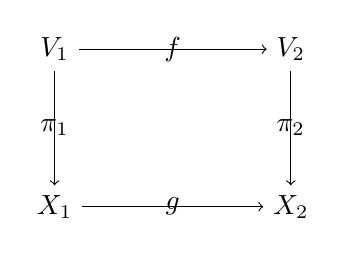
\begin{tikzpicture}
		\node (lt) {$V_1$};
		\node (rt) at (3,0) {$V_2$};
		\node (lb) at (0,-2) {$X_1$};
		\node (rb) at (3,-2) {$X_2$};
		\draw[->] (lt) to node {$f$} (rt);
		\draw[->] (lb) to node {$g$} (rb);
		\draw[->] (lt) to node [swap] {$\pi_1$} (lb);
		\draw[->] (rt) to node {$\pi_2$} (rb);
		\end{tikzpicture}
	\end{center}
	commutes and $f$ is fiberwise linear. That is, for every $x\in X_1$ the restriction of $f$ to $\pi_1^{-1}(x)$ is a linear map between the vector spaces $\pi_1^{-1}(x)$ and $\pi_2^{-1}(g(x))$.
	
	Note that $g$ is uniquely determined by $f$.
\end{defi}

\begin{defi}[$G$\=/linearisation, \phantom{}{\cite[chapter 1.3]{git}}]
	Let $G$ be an affine algebraic group acting on an affine variety $X$. Let $\pi\colon L \rightarrow X$ be a line bundle over $X$. A \emph{$G$\=/linearisation of $L$} is a morphism $(f,h)$ from the line bundle $G\times L$ to $L$ such that
	$$f\colon G\times L \longrightarrow L$$
	is an algebraic group action and
	\begin{center}
		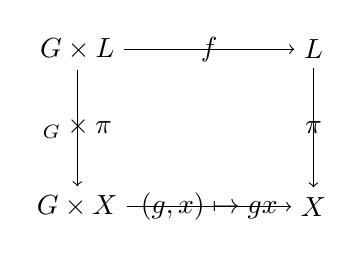
\begin{tikzpicture}
		\node (lt) {$G\times L$};
		\node (rt) at (3,0) {$L$};
		\node (lb) at (0,-2) {$G\times X$};
		\node (rb) at (3,-2) {$X$};
		\draw[->] (lt) to node {$f$} (rt);
		\draw[->] (lb) to node {$(g,x)\mapsto gx$} (rb);
		\draw[->] (lt) to node [swap] {$\id_G\times \pi$} (lb);
		\draw[->] (rt) to node {$\pi$} (rb);
		\end{tikzpicture}
	\end{center}
	commutes. A \emph{$G$\=/linearised line bundle} is a line bundle $L$ together with a  $G$\=/linearisation of $L$.
\end{defi}

\begin{remark}
	\label{remark:linearised_line_bundle_tensor}
	The tensor product $L_1 \tensor L_2$ of $G$\=/linearised line bundles $L_1$ and $L_2$ over $X$ with $G$\=/linearisations $f_1$, $f_2$ is the $G$\=/linearised line bundle that is obtained by taking the tensor product on the fibers. Its group action is given by tensoring the actions $f_1$ and $f_2$ restricted to the fibers. Note that $L_1^{\tensor n}$ is isomorphic to the line bundle $L_1$ with the $G$\=/linearisation
	$$G\times L_1 \longrightarrow L_1,\quad (g, \ell) \mapsto f_1(g^n, \ell)$$
\end{remark}

\begin{remark}[Group action on sections, \phantom{}{\cite[Remark 1.7]{git_equivalence}}]
	Let $L$ be a $G$\=/linearised line bundle over $X$. For each $G$\=/invariant open subset $U\subseteq X$ we obtain a group action of $G$ on the space $\Gamma(U,L)$ of sections over $U$ by setting
	$$(g\cdot s)(x) \defeq g\cdot s(g^{-1}x).$$
	The identity and compatibility axioms are verified easily. We check that $g\cdot s$ again is a section in $\Gamma(U,L)$. It is well defined on $U$ since we have $g^{-1}x\in U$ for all $g\in G$, $x\in U$. Clearly, $g\cdot s$ is the composition of morphisms and thus a morphism itself.
	
	The subspace of $G$\=/invariant sections of $L$ over $U$ is denoted by $\Gamma(U,L)^G$.
	\index{GammaULG@$\Gamma(U,L)^G$}%
\end{remark}

Now we are ready to describe the construction of semistable and stable points in accordance with \cite[Definition 1.7 \& 1.8]{git}. Note that for us, stable points mean properly stable points in the sense of Mumford.

\begin{defi}
	Let $L$ be a $G$\=/linearised, ample line bundle over $X$. A point $x\in X$ is called
	\begin{enumerate}[label={\upshape(\roman*)}]
		\item \emph{semistable} if there exists a $G$\=/invariant global section $s\in\Gamma(X,L^{\tensor n})^G$ for some $n\in\natural$ such that $s(x)\neq 0$, where $0$ is the origin in the fiber $\pi^{-1}(x)$.
		\item \emph{stable} if its stabiliser $G_x$ is finite and it is semistable via a global section $s$ such that all $G$\=/orbits in 
		$$X_s = X\setminus V(s) = \{p\in X\mid s(p) \neq 0 \}$$
		are closed.
	\end{enumerate}
	The sets of semistable points and stable points are denoted by $X^{ss}(L)$ and $X^{s}(L)$ respectively.
	\index{XssL@$X^{ss}(L)$}%
	\index{XsL@$X^{s}(L)$}%
\end{defi}

\begin{remark}
	\label{remark:semistable_points_yield_git_quotient}
	By Mumford, the $G$\=/invariant set $X^{ss}(L)$ permits a good quotient $X^{ss}(L)\sslash G$, called \emph{GIT quotient}. It is the projective variety of the graded ring
	$$\bigoplus_{n\geq 0} \Gamma(X,L^{\tensor n})^G.$$
	If  $X^{s}(L)$ is non\=/empty, $X^{ss}(L)\sslash G$ is an almost geometric quotient with the restriction to $X^{s}(L)$ being a geometric quotient.
\end{remark}

\section{The GIT fan}
\label{sec:git_fan}

The set of semistable points $X^{ss}(L)$ and the corresponding GIT quotient depend on the choice of a $G$\=/linearised line bundle. As we will see in this section, we are able to parametrise all nonempty sets of semistable points arising from linearisations of the trivial line bundle by a special quasifan, called GIT fan, whose cones are in inclusion\=/reversing one\=/to\=/one correspondence. We assume that the group $G$ is an algebraic torus acting on an affine variety $X$. Note that the general case of arbitrary connected reductive groups $G$ may be reduced to the torus case, see \cite[Lemma 3.3]{git_via_cox_rings}. The concepts presented here originate from \cite[chapter 2]{git_equivalence}.

For the remainder of this section we assume that $X$ is an affine variety with a $\integer^k$\=/grading on its ring $\O(X)$ of regular functions. It encodes an action of a $k$\=/dimensional torus $T$ by Construction~\ref{construction:algebraic_torus}.

\begin{lemma}[\phantom{}{\cite[Lemma 2.6]{git_equivalence}}]
	The $T$\=/linearisations of the trivial line bundle 
	$$\pi\colon X \times \field \rightarrow X$$
	correspond one\=/to\=/one to vectors in $\integer^k$, where $w\in\integer^k$ defines the $G$\=/linearisation
	\begin{equation}
		\label{equa:torus_linearisation}
		t\cdot(x,z) \defeq (t\cdot x, t^w z).
	\end{equation}
\end{lemma}
\begin{proof}
	One easily computes that (\ref{equa:torus_linearisation}) defines a $T$\=/linearisation for all $w\in\integer^k$. Now let $f:T\times X\times\field \rightarrow X\times\field$ be an arbitrary $T$\=/linearisation. Let $p_X$ and $p_\field$ be the projections of $X\times\field$ to $X$ and $\field$ respectively. Since $f$ is defined such that $\pi$ is equivariant, it follows that $p_X \circ f (t, x, z) = tx$. Furthermore, $p_\field \circ f(t,x,z)$ is linear w.r.t. $z$. For this reason there exists a morphism $c\colon T \times X \rightarrow \field$ such that
	$$p_\field \circ f(t,x,z)=c(t,x)z.$$
	Let $x\in X$. The compatibility axiom yields
	\begin{equation}
		\begin{aligned}
			c(t_1t_2, x) & = p_\field\circ f(t_1t_2, x, 1) \\
			& = p_\field(f(t_1, f(t_2, x, 1))) \\
			&= p_\field(f(t_1, t_2x, c(t_2,x))) \\
			&= c(t_1, t_2x)\cdot c(t_2, x).
		\end{aligned}
		\label{equa:torus_linearisation_compatibility}
	\end{equation}
	Due to the identity axiom and (\ref{equa:torus_linearisation_compatibility})
	$$1_\field = c(1_T, x) = c(t^{-1}, tx)\cdot c(t, x) \quad \forall (t,x)\in T\times X$$
	holds. In particular, $c$ does not vanish somewhere on $T\times X$, so that $c(\wildcard,x)$ becomes an invertible, rational function for every $x\in X$. By \cite[Proposition 3]{rationality_questiongs_algebraic_groups}, $c(\wildcard,x)$ is a character of $T$. As every character of $T$ is given by $t\mapsto t^\alpha$ for a suitable $\alpha\in\integer^d$ (see \cite[§16]{linear_algebraic_groups}), we conclude that 
	$$c = \sum_{\alpha\in I} t^\alpha \tensor f_\alpha \quad\text{with suitable}\ f_\alpha\in \O(X)\setminus\{0\}$$
	where for every $x\in X$ there exists exactly one $\alpha\in I$ such that $f_\alpha(x) = 1$ and $f_\beta(x) = 0$ for all $x\in I\setminus\{\alpha\}$.
	
	If $|I|>1$, we would obtain
	$$\bigcup_{\alpha\in I} V(f_\alpha) = X,$$
	contradicting the irreducibility of $X$. Thus, $I$ has to contain a single element which we denote by $w$. It follows that $c = t^w \tensor 1$.	
\end{proof}

\begin{notation}
	Let $w\in\integer^k$. We denote the $G$\=/linearised trivial line bundle corresponding to $w$ by $L_w$ and write $X(w)$ for the set of semistable points $X^{ss}(L_w)$.
	\index{Lomega@$L_w$}%
	\index{Xomega@$X(w)$}%
\end{notation}

Now that we have identified all GIT quotients arising from $T$\=/linearisations, we are going to complement them by a combinatorical description in terms of cones. A key role is assigned to orbit cones, from which finitely many exist. These contain all characters $w\in\integer^k$ of $T$ that permit a global section invariant w.r.t. to $L_w$ not vanishing on a fixed point $x\in X$. Non\=/empty intersections of orbit cones, called GIT cones, represent all non\=/empty sets of semistable points. Most interestingly, the collection of GIT cones form a quasifan with convex support. We exploit this fact later when giving an algorithmic solution for determining all GIT cones.

\begin{defi}[Orbit cone, \phantom{}{\cite[Definition 2.1]{git_equivalence}}]
	\label{defi:orbit_cone}
	Let $x\in X$. The \emph{orbit monoid} of $x$ is given by
	$$S_T(x) = \{w\in\integer^k\mid \exists f\in\O(X)_w\colon f(x) \neq 0\}.$$
	The convex, polyhedral cone $\omega_T(x)$ generated by $S_T(x)$ is called \emph{orbit cone} of $x$.
	\index{STx@$S_T(x)$}%
	\index{omegaTx@$\omega_T(x)$}%
	
	The \emph{weight cone} of $X$ is defined by
	$$\Omega_T(X) = \langle w\in\integer^k\mid \O(X)_w \neq 0 \rangle_{\rational_{\geq 0}}.$$
	Clearly, the union over all orbit cones is $\Omega_T(X)$.
	\index{OmegaTX@$\Omega_T(X)$}%
\end{defi}

\begin{lemma}
	Let $x\in X$. Then $S_T(x)$ indeed is a submonoid of $\integer^k$.
\end{lemma}
\begin{proof}
	Obviously, $0\in S_T(x)$ by considering $1$ in $\O(X)$. It remains to check that $S_T(x)$ is closed. Let $w_1, w_2\in S_T(x)$. Hence, there exist $f_1\in\O(X)_{w_1}$ and $f_2\in\O(X)_{w_2}$ with $f_1(x) \neq 0 \neq f_2(x)$.
	The product $f_1f_2$ is homogeneous of degree $w_1+w_2$ with $(f_1f_2)(x) \neq 0$. We conclude that $w_1+w_2\in S_T(x)$.
\end{proof}

\begin{prop}[\phantom{}{\cite[Proposition 2.5]{git_equivalence}}]
	\label{prop:finite_orbit_cones}
	The set of orbit cones $\{\omega_T(x)\mid x\in X\}$ is finite.
\end{prop}
\begin{proof}
	By Construction~\ref{construction:algebraic_torus}, we can embed $X$ into a suitable affine space $\field^m$ such that $\O(X)$ becomes the ring $\field[\mathbf{x}]/I(X)$ with grading
	$$\deg(x_i) = q_i\in\integer^k\quad\forall 1\leq i \leq m.$$
	Let $x\in X$ and $w\in\integer^k$ such that $w\in S_T(x)$. Then there exists a polynomial $f\in\field[\mathbf{x}]$ of degree $w$ with $f(x)\neq 0$. It follows that $f$ contains at least one monomial $\mathbf{x}^\alpha$ of degree $w$ that does not vanish when substituting $x$. In particular
	$$(t *_{(\field^*)^m} x)^\alpha = t^\alpha \cdot x^\alpha \neq 0$$
	for $t\in(\field^*)^m$, where $*_{(\field^*)^m}$ denotes the standard action of $(\field^*)^m$ on $\field^m$. We conclude that $S_T(x)$ is constant on $(\field^*)^m$\=/orbits over $\field^m$. Since there exist only a finite number of such orbits, the claim follows.
\end{proof}

\begin{lemma} Let $w\in\integer^k$. Then it holds that
	\label{lemma:semistable_points_determined_by_orbit_cones}
	\begin{align*}
	X(w) 
	&= \bigcup_{f\in\O(X)_{nw},\ n\in\natural} X_f\\
	&= \{x\in X\mid w\in\omega_T(x)\}.
	\end{align*}
\end{lemma}
\begin{proof}
	By Remark~\ref{remark:linearised_line_bundle_tensor}, we have $L_w^{\tensor n} = L_{nw}$ for all $n\in\natural$. Now fix $n\in\natural$ and let $s\in\Gamma(X,L_{nw})$ be a global section. Since we consider the (ample) trivial line bundle, $s$ corresponds to a morphism $f\in\O(X)$ such that
	$$s(x) = (x, f(x))\quad \forall x\in X.$$
	and $X_f$ contains all points with $s(x) \neq 0$. The section is $G$\=/invariant iff
	$$(tx, (t^{-1}f)(x)) = (tx, f(tx)) = s(tx) = (t\cdot s)(tx) = t\cdot s(x) = (tx, t^{nw} f(x))$$
	for all $t\in T$, $x\in X$. Taking Example~\ref{example:regular_functions_torus_group_action} into account, we obtain
	$$s\in\Gamma(X,L_{nw})^G \ \Longleftrightarrow\ f\in\O(X)_{nw}$$
	and the first equation follows. The inclusion $\subseteq$ of the second equation is obvious. For the other direction let $x\in X$ such that $w\in\omega_T(x)$. After eliminating denominators in a $\rational$\=/linear combination of $w$ over $S_T(x)$, one obtains $n\in\natural$ such that $nw \in S_T(x)$. The inclusion $\supseteq$ follows.
\end{proof}

\begin{coro} Let $w\in\integer^k$. The following conditions are equivalent:
	\begin{enumerate}[label={\upshape(\roman*)}]
	\item $X(w) \neq \emptyset$,
	\item $w\in\Omega_T(X)$.
	\end{enumerate}
\end{coro}
\begin{proof}
	Immediate consequence of Lemma~\ref{lemma:semistable_points_determined_by_orbit_cones} and the definition of the weight cone $\Omega_T(X)$.
\end{proof}

\begin{defi}[GIT cone, \phantom{}{\cite[Definition 2.8]{git_equivalence}}]
Let $w\in\Omega_T(X)$. The \emph{GIT cone} associated to $w$ is defined by
$$\sigma_T(w) = \bigcap_{w\in\omega_T(x)} \omega_T(x).$$
\index{sigmaTw@$\sigma_T(w)$}%

The collection of all GIT cones
$$\Sigma_T(X) \defeq \{\sigma_T(w)\mid w\in\Omega_T(X)\}$$
is called \emph{GIT fan}.
\index{SigmaTX@$\Sigma_T(X)$}%
\end{defi}

\begin{prop}[\phantom{}{\cite[Proposition 2.9]{git_equivalence}}]
	\label{prop:equivalence_git_cones_semistable_points}
	Let $w_1, w_2\in \Omega_T(x)$. Then
	$$X(w_1)\subseteq X(w_2) \ \Longleftrightarrow\ \sigma_T(w_1) \supseteq \sigma_T(w_2).$$
	In particular, $X(w_1) = X(w_2)$ if and only if $\sigma_T(w_1) = \sigma_T(w_2)$.
\end{prop}
\begin{proof}
	By Lemma~\ref{lemma:semistable_points_determined_by_orbit_cones} and the definition of GIT cones, for any $v,w\in\integer^k$ we have
	\begin{align*}
		v\in\sigma_T(w) &\ \Leftrightarrow\ v\in \omega_T(x)\quad \forall x\in X\ \mathrm{with}\ w\in\omega_T(x) \\
		&\ \Leftrightarrow\ v\in \omega_T(x)\quad \forall x\in X(w).
	\end{align*}
	The direction $\Rightarrow$ follows. For the converse, consider $X(w_1) \nsubseteq X(w_2)$ so that there exists $x\in X$ with $w_1\in \omega_T(x)$ and $w_2\notin \omega_T(x)$ by Lemma~\ref{lemma:semistable_points_determined_by_orbit_cones}. Since $\sigma_T(w_1)$ is a subset of $\omega_T(x)$, we conclude that $w_2\notin\sigma_T(w_1)$ and therefore $\sigma_T(w_2)\nsubseteq\sigma_T(w_1)$.
	
	The postscript immediately follows from the first claim.
\end{proof}

\begin{theorem}[\phantom{}{\cite[Theorem 2.11]{git_equivalence}}]
	\label{theorem:git_fan}
	The GIT fan $\Sigma_T(X)$ is a quasifan, that is a finite collection of convex polyhedral cones located in the same ambient space such that for $\sigma, \sigma'\in \Sigma_T(X)$
	\begin{enumerate}[label={\upshape(\roman*)}]
		\item all faces of $\sigma$ belong to $\Sigma_T(X)$,
		\item $\sigma \cap \sigma'$ is a face of both $\sigma$ and $\sigma'$.
	\end{enumerate}
	Its support
	$$|\Sigma_T(X)| \defeq \bigcup_{\sigma\in\Sigma_T(X)}\sigma$$
	is given by the (convex) weight cone $\Omega_T(X)$.
\end{theorem}

We postpone the proof and begin with some lemmas. Since the closure of a $T$\=/orbit in $X$ is $T$\=/invariant, it decomposes into a set of (possibly non\=/closed) $T$\=/orbits. The following lemma translates this setup into the world of orbit cones. We omit the proof and refer to \cite{git_equivalence}.

\begin{lemma}[\phantom{}{\cite[Corollary 2.4]{git_equivalence}}]
	\label{lemma:orbits_correspond_to_orbit_cones}
	The $T$\=/orbits in $X$ are in one\=/to\=/one correspondence with orbit cones via
	$$Ty \mapsto \omega_T(y).$$
	
	Let $x\in X$. Then all faces of $\omega_T(x)$ are orbit cones such that $\omega_T(y)$ is a face if and only if the corresponding $T$\=/orbit $Ty$ is located in $\overline{Tx}$.
\end{lemma}

\begin{notation}
	Let $\sigma\subseteq \rational^k$ be a cone. We write $\sigma^\circ$ for the relative interior of $\sigma$. Note that if $\sigma$ is of full dimension $k$, then the interior of $\sigma$ w.r.t.\ the euclidean topology coincides with the relative interior $\sigma^\circ$.
	\index{sigma°@$\sigma^\circ$}%
\end{notation}

\begin{lemma}[\phantom{}{\cite[Lemma 2.12]{git_equivalence}}]
	\label{lemma:git_cones_alternative_descriptions}
	Let $w\in\Omega	_T(X)$. Then it holds that
	\begin{enumerate}[label={\upshape(\roman*)}]
		\item $w\in \omega_T(x) \ \Leftrightarrow\ \sigma_T(w) \subseteq \omega_T(x)\quad \forall x\in X,$
		\label{enum_item:git_cone_in_all_orbit_cones}
		\item $w\in \omega_T(x)^\circ \ \Leftrightarrow\ \sigma_T(w)^\circ \subseteq \omega_T(x)^\circ\quad \forall x\in X,$
		\label{enum_item:git_cone_interior_in_all_orbit_cone_interiors}
		\item $\sigma_T(w) = \bigcap\limits_{w\in \omega_T(x)^\circ} \omega_T(x),$
		\label{enum_item:git_cone_intersection_wrt_interiors}
		\item $\sigma_T(w)^\circ = \bigcap\limits_{w\in \omega_T(x)^\circ} \omega_T(x)^\circ,$
		\label{enum_item:git_cone_interior}
		\item $w\in\sigma_T(w)^\circ.$
		\label{enum_item:git_cone_generator_in_interior}
	\end{enumerate}
\end{lemma}
\begin{proof}
	\ref{enum_item:git_cone_in_all_orbit_cones} immediately follows from the definition of GIT cones.
	
	For any orbit cone $\omega_T(x)$ with $w\in\omega_T(x)$ there exists a minimal face $\omega\preceq \omega_T(x)$ containing $w$ in its relative interior. Since $\omega$ is an orbit cone by Lemma~\ref{lemma:orbits_correspond_to_orbit_cones}, it suffices to intersect with orbit cones containing $w$ in its interior, showing \ref{enum_item:git_cone_intersection_wrt_interiors}.
	
	\ref{enum_item:git_cone_interior} and \ref{enum_item:git_cone_generator_in_interior} are a consequence of the following fact: If the intersection of the relative interiors of a finite number of convex polyhedral cones is non\=/empty, then it equals the relative interior of the intersection of the cones. \ref{enum_item:git_cone_interior_in_all_orbit_cone_interiors} follows from \ref{enum_item:git_cone_interior} and \ref{enum_item:git_cone_generator_in_interior}.
\end{proof}

\begin{lemma}[\phantom{}{\cite[Proof of Theorem 2.11]{git_equivalence}}]
	\label{lemma:git_cone_subsets_of_git_cones_are_faces}
	Let $w_1,w_2\in\Omega_T(X)$. Then the inclusion $\sigma_T(w_1) \subseteq \sigma_T(w_2)$ implies $\sigma_T(w_1) \preceq \sigma_T(w_2)$.
\end{lemma}
\begin{proof}
	 Let $\omega_T(x_1),\dots,\omega_T(x_r)$ be the orbit cones with $\sigma_T(w_1)^\circ \subseteq \omega_T(x_i)^\circ$ for $1\leq i \leq r$. By Lemma~\ref{lemma:git_cones_alternative_descriptions}, we have $\sigma_T(w_1) = \omega_T(x_1) \cap \cdots \cap \omega_T(x_r)$.
	 
	 Choose representatives $x_1,y_1,\dots,y_\ell$ of the $T$\=/orbit decomposition of $\overline{Tx_1}$.
	 Then Lemma~\ref{lemma:orbits_correspond_to_orbit_cones} states that $\omega_T(y_i) \preceq \omega_T(x_1)$ is a proper face for all $1\leq i \leq \ell$. Because of $\sigma_T(w_1)^\circ \subseteq \omega_T(x_1)^\circ$, it follows that $\omega_T(y_i) \cap \sigma_T(w_1)^\circ = \emptyset$. By Lemma~\ref{lemma:git_cones_alternative_descriptions}, $w_1$ is contained in $\sigma_T(w_1)^\circ$ but not in $\omega_T(y_i)$. For this reason $y_i\notin X(w_1)$ holds. Together with $x_1\in X(w_1)$ due to $w_1\in \sigma_T(w_1)^\circ \subseteq \omega_T(x_1)^\circ$, we conclude that
	 \begin{equation}
		 \label{equa:orbit_closed_in_Xw1}
		 \overline{Tx_1} \cap X(w_1) = Tx_1,
	 \end{equation}
	 i.e. $Tx_1$ is closed in $X(w_1)$.
	 
	 By Proposition~\ref{prop:equivalence_git_cones_semistable_points}, we have $X(w_2)\subseteq X(w_1)$. We denote the good quotient maps of $X(w_1)$ and $X(w_2)$ by $p_1$ and $p_2$ respectively. The morphism
	 $$\varphi: X(w_2) \hookrightarrow X(w_1) \rightarrow X(w_1) \sslash T$$
	 is $G$\=/invariant. Hence, the universal property of categorical quotients yields a unique morphism $\psi: X(w_2)\sslash T \rightarrow X(w_1)\sslash T$ such that the diagram
	 \begin{center}
	 	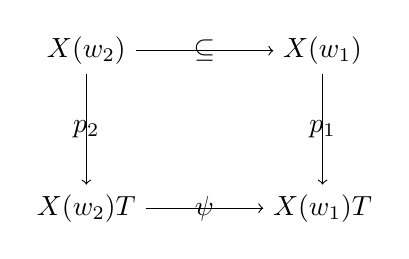
\begin{tikzpicture}
	 	\node (lt) {$X(w_2)$};
	 	\node (rt) at (3,0) {$X(w_1)$};
	 	\node (lb) at (0,-2) {$X(w_2) \sslash T$};
	 	\node (rb) at (3,-2) {$X(w_1) \sslash T$};
	 	\draw[->] (lt) to node {$\subseteq$} (rt);
	 	\draw[->] (lb) to node {$\psi$} (rb);
	 	\draw[->] (lt) to node [swap] {$p_2$} (lb);
	 	\draw[->] (rt) to node {$p_1$} (rb);
	 	\end{tikzpicture}
	 \end{center}
	 commutes. Since both $X(w_1) \sslash T$ and $X(w_2) \sslash T$ are projective over $\O(X)_0$ due to Remark~\ref{remark:semistable_points_yield_git_quotient}, $\psi$ is projective with closed image in $X(w_1) \sslash T$. Furthermore, $X(w_2)$ is a $G$\=/invariant, dense open subset of $X(w_1)$. By the definition of good quotients, the image of the closed complement $X(w_1)\setminus X(w_2)$ under $p_1$ is closed. Proposition~\ref{prop:good_quotient_properties} shows that $p_1$ is surjective, so that the image of $X(w_2)$ under $p_1$, which is the image of $\psi$, contains a non\=/empty open subset and thus is dense. Overall it follows that $\psi$ is surjective. 
	 
	 Now, there exists a point $z_1\in X(w_2) \cap p_1^{-1}(p_1(x_1))$. By Proposition~\ref{prop:good_quotient_properties}, it follows that 
	 $$\overline{Tx_1} \cap \overline{Tz_1} \cap X(w_1) \neq \emptyset.$$
	 Applying (\ref{equa:orbit_closed_in_Xw1}) yields
	 $$Tx_1 \cap \overline{Tz_1} \neq \emptyset$$
	 which results in
	 $$Tx_1 \subseteq \overline{Tz_1}.$$
	 By Lemma~\ref{lemma:orbits_correspond_to_orbit_cones}, $\omega_T(x_1)$ is a face of $\omega_T(z_1)$. Because of $z_1\in X(w_2)$, it holds that $w_2\in \omega_T(z_1)$, that is $\sigma_T(w_2) \subseteq \omega_T(z_1)$ by Lemma~\ref{lemma:git_cones_alternative_descriptions}. Repeating the process for $x_2,\dots,x_r$ yields orbit cones $\omega_T(z_i)$ such that $\omega_T(x_i)\preceq \omega_T(z_i)$ and $\sigma_T(w_2) \subseteq \omega_T(z_i)$ for all $1\leq i\leq r$.
	 
	 Now let $\tau\preceq \sigma_T(w_2)$ be the unique face with $\sigma_T(w_1)^\circ \subseteq \tau^\circ$ by Lemma~\ref{lemma:cones_in_cones}. In particular,
	 $$\tau\subseteq\omega_T(z_i)\quad\mathrm{and}\quad\emptyset \neq \sigma_T(w_1)^\circ \subseteq \tau^\circ \cap \omega_T(x_i)^\circ$$
	 hold for all $1\leq i\leq r$. Again by Lemma~\ref{lemma:cones_in_cones}, we conclude that $\tau\subseteq \omega_T(x_i)$. It follows that $\tau \subseteq \sigma_T(w_1)$. The equality is obtained by taking closures in $\sigma_T(w_1)^\circ \subseteq \tau^\circ$. Hence, $\sigma_T(w_1) = \tau$ is a face of $\sigma_T(w_2)$.
\end{proof}

Now we are ready to proof Theorem~\ref{theorem:git_fan}.
\begin{proof}
	The finiteness of $\Sigma_T(X)$ is an immediate consequence of Proposition~\ref{prop:finite_orbit_cones}. 
	
	Let $\sigma\in\Sigma_T(X)$ be a GIT cone and $\sigma_0\preceq\sigma_T(w)$ be a face. Choose $w\in\sigma_0^\circ$. By Lemma~\ref{lemma:git_cones_alternative_descriptions}, $\sigma$ is the intersection of all orbit cones containing $\sigma$. These also contain $w$, hence $\sigma_T(w)\subseteq \sigma$ by the definition of GIT cones. The prerequisite of Lemma~\ref{lemma:git_cone_subsets_of_git_cones_are_faces} is satisfied so that $\sigma_T(w)\preceq \sigma$. Now, $\sigma_T(w)$ and $\sigma_0$ are both faces of $\sigma$ containing $w$ in their relative interior by Lemma~\ref{lemma:git_cones_alternative_descriptions}. This may only be the case when $\sigma_0 = \sigma_T(w)$, proving that $\sigma_0\in\Sigma_T(X)$.
	
	Next, let $\sigma_1,\sigma_2\in\Sigma_T(X)$. Let $\tau_i\preceq\sigma_i$ be the unique face such that $(\sigma_1\cap\sigma_2)^\circ \subseteq \tau_i^\circ$ by Lemma~\ref{lemma:cones_in_cones} ($i=1,2$). Let $w\in(\sigma_1\cap\sigma_2)^\circ$. In particular, it holds that $w\in\tau_i^\circ$, so that we obtain $\sigma_T(w) = \tau_i$ and $\sigma_T(w)\subseteq \sigma_i$ as before. Due to $\sigma_1 \cap \sigma_2 \subseteq \tau_i$, it follows that 
	$$\sigma_1 \cap \sigma_2 = \tau_1 = \tau_2 = \sigma_T(w).$$
	For this reason, $\sigma_1 \cap \sigma_2$ is a face of both $\sigma_1$ and $\sigma_2$.
\end{proof}
	\chapter{Concept of the algorithm}
\label{chap:algorithm}

In the following sections we are going to develop a mathematical and algorithmic framework that allows us to compute the GIT fan for the case of a torus acting on an affine variety. The concepts presented in this chapter base on \cite{gitfan_symmetry, gitfan}.

First, we describe the formal setup and introduce the notation being used in the upcoming chapters. In the second section we present an algorithm that is capable of identifying orbit cones. They play an important role in the theory since all GIT cones emerge from their intersections. Afterwards, we transform the problem of computing the GIT fan into the problem of traversing a graph and present a suitable algorithm. Third, we modify the previous algorithms such that symmetries of the affine variety may be exploited in order to reduce the problem size by a factor that relates to the size of the symmetry group. Finally, we give an counterexample that -- contrary to \cite{gitfan_symmetry} -- one cannot drop non-minimal orbit cones with respect to inclusion. For this reason, we leave out the minimisation process.

\section{The setup}
\label{section:setup}

Let $\field$ be an algebraically closed field of characteristic zero. We consider an algebraic group action of a $k$-dimensional torus $T$ on an affine variety $X$. Due to construction~\ref{construction:algebraic_torus}, we describe this setup by a set of integral vectors $q_i\in\integer^k$, $1\leq i \leq r$, and a suitable embedding of $X$ in $\field^r$ such that its vanishing ideal $\ideal \defeq I(X)$ is homogeneous w.r.t.
$$\deg(x_i) = q_i,\quad 1\leq i \leq r.$$
The vectors $q_i$ form the columns of a matrix $Q\in\field^{k\times r}$. By restricting $T$ to a lower dimensional subtorus if necessary, we may assume that $Q$ has rank $k$ without changing the orbits in $X$. Furthermore, we assume that $\ideal$ contains no monomials. As we will see later on, this assumption is equivalent to $X\cap (\field^*)^r \neq \emptyset$. On that account and the irreducibility of $X$, $X$ is located in at least one of the hyperplanes $\{x_i = 0\}$, $1\leq i \leq r$, iff the assumption does not hold. By ``forgetting" all variables with $X\cap \{x_i = 0\} = X$, we obtain an embedding of $X$ such that $X\cap (\field^*)^{r'} \neq \emptyset$ holds.

\section{Computing orbit cones}

In this section we describe orbit cones by faces of the positive orthant $\rational_{\geq 0}^r$, which we denote by $\gamma$.
\index{gamma@$\gamma$}%
From a combinatorial point of view these faces are subsets of $\{1,\dots,r\}$ such that whenever $e_i$ is a ray of a face, $i$ is located in the corresponding subset. A face $\gamma_0 \preceq \gamma$ defines a restriction $z_{\gamma_0}$ of any $r$\=/tuple of objects $z=(z_1,\dots,z_r)$ by setting
$$(z_{\gamma_0})_i =
\begin{cases}
z_i, & e_i\in\gamma_0 \\
0, & \text{else}
\end{cases}\quad 1\leq i \leq r.$$
We write $\ideal_{\gamma_0}$ for the ideal in $\field[\mathbf{x}_{\gamma_0}]$ that is obtained by sending all $x_i$ in $\ideal$ with $x_i\notin\gamma_0$ to zero.
\index{agamma0@$\ideal_{\gamma_0}$}%
Additionally, we define
$$\T_{\gamma_0} \defeq (\field^*)^r \cdot (1,\dots,1)_{\gamma_0},$$
which is the torus corresponding to $\gamma_0$.
\index{Tgamma0@$\T_{\gamma_0}$}%

\begin{defi}[\aface]
	A face $\gamma_0\preceq\gamma$ is called \emph{\aface{}} iff $X\cap \T_{\gamma_0} \neq \emptyset$.
	\index{aface@\aface}%
\end{defi}

\begin{prop}
	\label{prop:aface_orbit_cone_correspondence}
	The set
	$$\Omega_\ideal \defeq \left\{Q(\gamma_0)\ |\ \gamma_0\preceq\gamma \text{ is an } \ideal\text{\=/face}\right\}$$
	equals the collection of orbit cones as in Definition~\ref{defi:orbit_cone}.
	\index{Oa@$\Omega_\ideal$}%
\end{prop}
\begin{proof}
	Let $x\in X$. Set $I_x = \{1 \leq i \leq r\ |\ x_i \neq 0\}$ and $J_x = \{1 \leq i \leq r\ |\ x_i = 0\}$. We claim that
	$$S_T(x) = \langle q_i\ |\ i\in I_x\rangle.$$
	
	Let $i\in I_x$. Since $x_i\in\field[\mathbf{x}]$ does not send $x$ to zero, we have
	$$q_i = \deg(x_i)\in S_T(x).$$
	Now let $w\in S_T(x)$. Then there exists $f\in\field[\mathbf{x}]_w$ such that $f(x) \neq 0$. In particular, at least one monomial $\mathbf{x}^\alpha$ of $f$ does not send $x$ to zero, thus $\alpha_j = 0$ for all $j\in J_x$. On that account we have
	$$w = \deg(x^\alpha) = \sum_{i=1}^r \alpha_i q_i = \sum_{i\in I_x} \alpha_i q_i,$$
	proving the claim.
	
	If $\gamma_0\preceq\gamma$ is an \aface{}, we find a point $x\in X\cap \T_{\gamma_0}$. By the previous claim, its orbit monoid is generated by the columns $q_i$ of $Q$ with $e_i\in\gamma_0$. Consequently, $Q(\gamma_0)$ is the orbit cone of $x$ generated by $S_T(x)$.
	
	Conversely, consider the orbit cone of an arbitrary point $x\in X$. Let $\gamma_x$ be the face of $\gamma$ that is generated by the rays $e_i$ with $i\in I_x$. Then $\gamma_x$ is an \aface{}, since $x\in X\cap \T_{\gamma_x}$. With the same arguments as before, it follows that $Q(\gamma_x)$ is the orbit cone of $x$.
\end{proof}

The previous proposition shows that all orbit cones arise from \afaces{} and that every \aface{} yields an orbit cone. Thus, if we are able to develop computable criteria in order to implement a test for the \aface{} property, we can derive all orbit cones by applying $Q$. The next proposition provides us with a suitable criterion.

\begin{prop}
	\label{prop:aface_equivalence}
	Let $\gamma_0\preceq\gamma$ be a face and $I= \{1\leq i\leq r\ |\ e_i\in\gamma_0\}$. Then the following conditions are equivalent:
	\begin{enumerate}[label={\upshape(\roman*)}]
		\item $\gamma_0$ is an \aface{}, that is $X\cap \T_{\gamma_0} \neq \emptyset$,
		\label{enum_item:aface_equivalence_aface}
		\item $\ideal_{\gamma_0}$ does not contain a monomial,
		\label{enum_item:aface_equivalence_monomial}
		\item $(\ideal_{\gamma_0} : (\prod_{i\in I} x_i)^\infty) = \field[\mathbf{x}_{\gamma_0}]$.
		\label{enum_item:aface_equivalence_saturation}
	\end{enumerate}
\end{prop}
\begin{proof}
	\ref{enum_item:aface_equivalence_monomial} $\Leftrightarrow$ \ref{enum_item:aface_equivalence_saturation} immediately follows from the definition of saturated ideals (see Appendix~\ref{appendix:ideal_quotients}), which unravels to
	$$\left(\ideal_{\gamma_0} : \left(\prod_{i\in I} x_i\right)^\infty\right) = \left\{r\in \field[\mathbf{x}]\ \middle|\ \exists j\in\natural: r\cdot \left(\prod_{i\in I} x_i\right)^j \in \ideal_{\gamma_0}\right\}.$$
	If $\ideal_{\gamma_0}$ contains a monomial $x^\alpha$, we have that $(\prod_{i\in I} x_i)^j\in\ideal_{\gamma_0}$, where $j$ is the largest integer occurring in $\alpha$. Thus, $1\in (\ideal_{\gamma_0} : (\prod_{i\in I} x_i)^\infty)$ and therefore \ref{enum_item:aface_equivalence_saturation} follows. Otherwise, if \ref{enum_item:aface_equivalence_saturation} holds, a power of $\prod_{i\in I} x_i$, which is a monomial, is contained in $\ideal_{\gamma_0}$.
	
	\ref{enum_item:aface_equivalence_aface} $\Rightarrow$ 
	\ref{enum_item:aface_equivalence_monomial}: Choose a point $x\in X\cap \T_{\gamma_0}$. Assume that \ref{enum_item:aface_equivalence_monomial} does not hold, i.e. $\ideal_{\gamma_0}$ contains a monomial $\mathbf{x}^\alpha$, $\alpha = (\alpha_i)_{i\in I}$, that is obtained by sending all $x_i$, $i\notin I$, in a suitable $f\in\ideal$ to zero.
	Since $x\in\T_{\gamma_0}$, it holds that
	$$f(x) = \prod_{i\in I} x_i^{\alpha_i} \neq 0,$$
	contradicting $x\in X = V(\ideal)$.
	
	\ref{enum_item:aface_equivalence_monomial} $\Rightarrow$ 
	\ref{enum_item:aface_equivalence_aface}: Assume that $V(\ideal_{\gamma_0}) \subseteq V(\prod_{i\in I} x_i)$ holds. Then Hilbert's Nullstellensatz yields $j\in\natural$ such that $(\prod_{i\in I} x_i)^j\in\ideal_{\gamma_0}$, contradicting \ref{enum_item:aface_equivalence_monomial}. Hence, $V(\ideal_{\gamma_0}) \not\subseteq V(\prod_{i\in I} x_i)$. In particular, we find a point $z = (z_i)_{i\in I} \subseteq \field^*$ with $z\in V(\ideal_{\gamma_0})$. We extend $z$ to a point $\tilde{z}\in\T_{\gamma_0}$ by setting
	$$\tilde{z}_i = \begin{cases}
	z_i, & i\in I \\
	0, & \text{else}
	\end{cases}\quad 1\leq i \leq r.$$
	
	Let $f\in\ideal$ and $f_{\gamma_0}\in\ideal_{\gamma_0}$ be the reduction of $f$ by sending all variables $x_i$, $i\notin I$, to zero. Then we have
	$$f(\tilde{z}) = f_{\gamma_0}(z) = 0,$$
	since $z\in V(\ideal_{\gamma_0})$. We conclude that $\tilde{z}\in X$, showing \ref{enum_item:aface_equivalence_aface}.
\end{proof}

Next, we implement an algorithm computing $(I : (z_1\cdots z_n)^\infty)$ for arbitrary ideals $I\in\field[z_1,\dots,z_n]$. The algorithm presented here originates from \cite{gitfan_symmetry} and has been implemented in \gitfanlib. It relies on the following proposition that allows us to compute $(I : (z_i)^\infty)$ with relative ease by a small modification to the Buchberger's algorithm.

\begin{prop}[\phantom{}{\cite[Proposition 3.1]{gitfan_symmetry}}]
	\label{proposition:saturated_monomial}
	Let $\;>$ be a monomial ordering on $\field[\mathbf{z}]$ and $\mathcal{G}$ be a standard basis of $I$ with respect to $\;>$. Let $m\in\{1,\dots,n\}$. If $\;>$ satisfies
	\begin{equation}
		\label{equation:saturated_monomial_assumption}
		z_m \mid f\ \Leftrightarrow\ z_m \mid \text{LM}_>(f),
	\end{equation}
	then
	$$\left\{g\in\field[\mathbf{z}]\ \middle|\ z_m \centernot\mid g\ \mathrm{and}\ \exists i\in\natural_0: (z_m)^i \cdot g \in \mathcal{G}\right\}$$
	is a standard basis for the saturated ideal $I : (z_m)^\infty$. 
\end{prop}

\begin{remark}
	\label{remark:satisying_assumption_saturated_monomial}
	The negative reverse lexicographical ordering
	$$z^\alpha >_\text{rs} z^\beta\ \defequiv\ \exists i\in\{1,\dots,n\}: \alpha_i < \beta_i\ \text{and}\ \alpha_j = \beta_j\ \forall j\in\{i+1,\dots,n\}$$
	ensures that (\ref{equation:saturated_monomial_assumption}) is satisfied for $m=n$. Every monomial $z^\beta$ with $z_n \mid z^\beta$ is strictly smaller than any monomial $z^\alpha$ with $z_n \centernot\mid z^\alpha$, since $\alpha_n = 0 < \beta_n$. Note that (\ref{equation:saturated_monomial_assumption}) may hold for other values of $m$ by using a negative reverse lexicographical ordering after reordering the variables $z_1,\dots,z_n$.
	
	Unfortunately, $\;>_\text{rs}$ is no global ordering. However, if $I$ permits a weight vector $w\in\integer^n_{>0}$ such that $I$ is homogeneous, we consider the $w$\=/weighted degree ordering with tie-breaker $\;>_\text{rs}$, that is $(>_w, >_\text{rs})$. This ordering is global and satisfies (\ref{equation:saturated_monomial_assumption}) on $w$\=/homogeneous generators of $I$.
\end{remark}

Since we have
$$(I:(z_1\cdots z_n)^\infty) = (\dots((I:(z_1)^\infty):(z_2)^\infty):\dots : (z_n)^\infty)\quad\text{(see Appendix \ref{appendix:ideal_quotients})},$$
Proposition~\ref{proposition:saturated_monomial} allows us to compute $(I : (z_1\cdots z_n)^\infty)$ by alternating Mora's algorithm with $>_\text{rs}$ and the elimination of factors $z_i$. If a global ordering as in Remark~\ref{remark:satisying_assumption_saturated_monomial} is available, one can integrate the elimination process into the Buchberger's algorithm in order to speed up convergence. Algorithm~\ref{algo:saturated_monomial} (see also \cite[Algorithm 3.3]{gitfan_symmetry}) contains the necessary modifications.

\begin{algorithm}
	\caption{Computing the saturation at the product of all variables}
	\label{algo:saturated_monomial}
	
	\KwIn{A vector $w\in\integer^n_{>0}$ and a set $\mathcal{G}$ of $w$-homogenous polynomials such that $\langle \mathcal{G}\rangle = I$}
	\KwOut{A Gröbner basis for the saturation $(I:(z_1\cdots z_n)^\infty)$ with respect to the ordering $(>_w, >_\text{rs})$}
	\BlankLine
	$\mathcal{G} \leftarrow \{g / z^\alpha\ |\ g\in \mathcal{G}\ \text{and}\ \alpha\ \text{maximal such that}\ z^\alpha \mid g\}$\;
	\label{algo_line:saturated_monomial_preprocess_G}
	\For{$m=1,\dots,n$}{
		Let $\;>_m$ be $(>_w, >_\text{rs})$ where $\;>_\text{rs}$ is the negative reverse lexicographical ordering after reordering variables such that
		$$z_1 >_\text{rs} \dots >_\text{rs} z_{m-1} >_\text{rs} z_{m+1} >_\text{rs} \dots >_\text{rs} z_n >_\text{rs} z_m.$$
		
		\Repeat{$\mathcal{G} = \mathcal{H}$\label{algo_line:saturated_monomial_repeat_condition}}{
			$\mathcal{H} \leftarrow \mathcal{G}$\;
			\For{$f,g\in\mathcal{H}$}{
				$r \leftarrow \text{NF}_{>_m} (\text{spoly}_{>_m}(f,g),\mathcal{H})$\;
				\If{$r \neq 0$}{
					$r \leftarrow r / z^\alpha,\ \text{where}\ \alpha\ \text{is maximal such that}\ z^\alpha \mid g$\;
					$\mathcal{G} \leftarrow \mathcal{G} \cup \{r\}$\;
				}
			}
		}
	}
	\Return $\mathcal{G}$\;
\end{algorithm}

\begin{prop}
	Algorithm~\ref{algo:saturated_monomial} computes the saturation $(I:(z_1\cdots z_n)^\infty)$ as specified in pseudo code.
\end{prop}
\begin{proof}
	Similarly to the Buchberger's algorithm, whenever a new element $r$ is introduced to $\mathcal{G}$, its lead monomial $\text{LM}(r)$ is not contained in the lead ideal of $\langle \mathcal{G} \rangle$. Consequently, $\langle \mathcal{G} \rangle$ strictly increases. Since $\field[\mathbf{z}]$ is noetherian, eventually $\langle \mathcal{G} \rangle$ becomes stationary, implying that no new elements $r$ have been inserted. Hence, the condition in Line~\ref{algo_line:saturated_monomial_repeat_condition} holds eventually and the algorithm terminates.
	
	Denote by $\mathcal{G}_0$ the set $\mathcal{G}$ after executing Line~\ref{algo_line:saturated_monomial_preprocess_G} and by $\mathcal{G}_m$ the Gröbner basis after the $m$-iteration of the outmost loop. Set $I_m = \langle \mathcal{G}_m \rangle$.
	
	First, note that the elements inserted into $\mathcal{G}$ are contained in $(I:(z_1\cdots z_n)^\infty)$ and are not divisible by any monomials. Furthermore, they are $w$-homogeneous since NF and spoly preseve homogeneity. Consequently, $\mathcal{G}_m$ satisfies the assumption of Proposition~\ref{proposition:saturated_monomial} with respect to the ordering $\;>_m$. As no element of $\mathcal{G}_m$ is divisible by any monomial, it follows that $\mathcal{G}_m$ is saturated with respect to $z_m$. In particular, $(I_{m-1} : (z_m)^\infty) \subseteq I_m$. Appendix~\ref{appendix:ideal_quotients} states that saturations preserve inclusion, so that $I\subseteq I_0$ together with $(I_{m-1} : (z_m)^\infty) \subseteq I_m$ implies that
	$$(I:(z_1\cdots z_n)^\infty) = (\dots((I:(z_1)^\infty):(z_2)^\infty):\dots : (z_n)^\infty) \subseteq I_n$$
	by a simple induction. It follows that $\langle \mathcal{G}_m \rangle = I_m = (I:(z_1\cdots z_n)^\infty)$.
\end{proof}

Now we are able to compute all orbit cones $\Omega_\ideal^{(k)}$ of full dimension $k$ by Algorithm~\ref{algo:compute_orbit_cones}. Its correctness is a straightforward conclusion from  Proposition~\ref{prop:aface_orbit_cone_correspondence} and~\ref{prop:aface_equivalence}.

\begin{notation}
	Let $\mathcal{C}$ be a set of convex cones. Then we write $\mathcal{C}^{(k)}$ for the subset of all $k$\=/dimensional cones in $\mathcal{C}$.
	\index{C(k)@$\mathcal{C}^{(k)}$}%
\end{notation}

\begin{algorithm}
	\caption{Computing all full dimensional orbit cones}
	\label{algo:compute_orbit_cones}
	
	\KwIn{$\ideal$, $Q$}
	\KwOut{All orbit cones of $\Omega_\ideal^{(k)}$ dimension $k$}
	\BlankLine
	$\Omega \leftarrow \emptyset$\;
	\For{$\gamma_0\preceq \gamma$ with $\dim(Q(\gamma_0)) = k$}{
		$I \leftarrow \ideal_{\gamma_0}$\;
		$I_\text{sat} \leftarrow (I:(\prod_{e_i\in\gamma_0} x_i)^\infty)$%
			\Comment*[r]{by Algorithm~\ref{algo:saturated_monomial}}
		\If{$I_\text{sat} = \field[\mathbf{x}_{\gamma_0}]$}{
			$\Omega \leftarrow \Omega \cup \{Q(\gamma_0)\}$\;
		}
	}
	\Return $\Omega$\;
\end{algorithm}

\section{Traversing the GIT fan}

With the full dimensional orbit cones at hand, we are able to determine the GIT fan $\Sigma_T(X)$ defined by the torus action $T$ on the variety $X$. Since the support of $\Sigma_T(X)$ is the image $Q(\gamma)$ and $Q$ has rank $k$, it follows that $\Sigma_T(X)$ is a $k$-dimensional quasifan with convex support.
By Lemma~\ref{lemma:convex_fan_maximal_cones}, it suffices to consider only the full dimensional GIT cones in $\Sigma_T(X)^{(k)}$. These yield a graph structure by relating two GIT cones sharing a common facet.

\begin{defi}
	The graph $\mathcal{G}(\Sigma_T(X))$ of the GIT fan $\Sigma_T(X)$ is the undirected graph with nodes in $\Sigma_T(X)^{(k)}$ and the symmetric relation
	$$E_{\mathcal{G}(\Sigma_T(X))} \defeq \left\{\{\lambda, \mu\} \mid \lambda, \mu \in \Sigma_T(X)^{(k)} \text{ and }\lambda \cap \mu \text{ is a facet of both }\lambda\text{ and }\mu\right\}.$$
	\index{GSigmaTX@$\mathcal{G}(\Sigma_T(X))$}%
	\index{EGSigmaTX@$E_{\mathcal{G}(\Sigma_T(X))}$}%
\end{defi}

\begin{prop}
	\label{proposition:git_fan_connected}
	The graph $\mathcal{G}(\Sigma_T(X))$ is connected.
\end{prop}
\begin{proof}
	Let $\lambda_s, \lambda_t\in\Sigma_T(X)^{(k)}$ and choose a point $x_s\in\lambda_s^\circ$. Let $S$ be the set of points that are not located on a line through $x_s$ and a point of a face of dimension $k-2$ or lower, that is
	$$S = \left\{p\in|\Sigma|\ \middle|\ \overline{x_s p} \cap \left(\bigcup_{\lambda\in\Sigma_T(X)^{(\leq k-2)}} \lambda\right) = \emptyset\right\}.$$
	Obviously, for every point $p\in |\Sigma|\setminus S$ we can choose $\lambda\in\Sigma_T(X)^{(\leq k-2)}$ such that $p$ is located in the subspace generated by $x_s$ and $\lambda$. As the dimension of this subspace is at most $k-1$, we conclude that the complement of $S$ in $|\Sigma|$ is contained in a finite union of hyperplanes.
	For dimensional reasons, any non\=/empty open set $U$ in $|\Sigma|$ with respect to the euclidean topology satisfies
	$$U\cap S \neq \emptyset.$$
	This shows that there exists a point $x_t\in\lambda_t^\circ$ such that $x_t\in S$.
	
	Consider the connecting line $\ell \defeq \overline{x_s x_t}$. We have $\ell\subseteq|\Sigma_T(X)|$, because $|\Sigma_T(X)|$ is convex. By the definition of $S$, $\ell$ only contains points in the relative interior of $(k-1)$- or $k$\=/dimensional cones. Furthermore, $\ell$ intersects every $(k-1)$\=/dimensional cone $\lambda$ in at most one point. Otherwise, $\ell$ would be contained in the hyperplane spanned by $\lambda$ due to Bézout's theorem. Then, $\ell$ also would intersect a proper face of $\lambda$ with dimension lower than $k-1$, contradicting $x_t\in S$.
	
	Since the relative interior of a $k$\=/dimensional cone is open and convex, its intersection with $\ell$ is an open interval in $\ell$. We conclude that $\ell$ has the form
	
	\begin{center}
		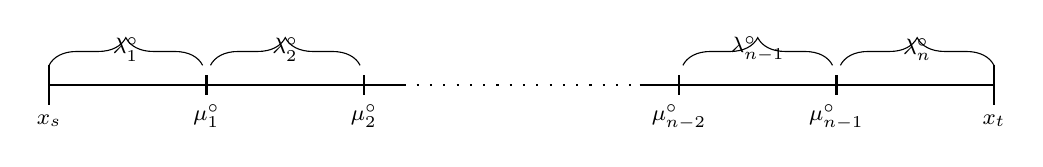
\begin{tikzpicture}
		\draw[thick] (0,0) -- (4.5,0);
		\draw[thick,loosely dotted] (4.5,0) -- (7.5,0);
		\draw[thick] (7.5,0) -- (12,0);
		\draw[thick] (0,-0.25) -- (0,0.25);
		\draw[thick] (12,-0.25) -- (12,0.25);
		\draw[thick] (2,-0.125) -- (2,0.125);
		\draw[thick] (4,-0.125) -- (4,0.125);
		\draw[thick] (8,-0.125) -- (8,0.125);
		\draw[thick] (10,-0.125) -- (10,0.125);
		
		\draw[decorate,decoration={brace,amplitude=10pt}]
			(0,0.25) -- (1.95,0.25) node [midway, yshift=0.2cm] {\footnotesize $\lambda_1^\circ$};
			\draw[decorate,decoration={brace,amplitude=10pt}]
			(2.05,0.25) -- (3.95,0.25) node [midway, yshift=0.2cm] {\footnotesize $\lambda_2^\circ$};
			\draw[decorate,decoration={brace,amplitude=10pt}]
			(8.05,0.25) -- (9.95,0.25) node [midway, yshift=0.2cm] {\footnotesize $\lambda_{n-1}^\circ$};
			\draw[decorate,decoration={brace,amplitude=10pt}]
			(10.05,0.25) -- (12,0.25) node [midway, yshift=0.2cm] {\footnotesize $\lambda_n^\circ$};
		\node[anchor=north] at (0,-0.25) {\footnotesize $x_s$};
		\node[anchor=north] at (2,-0.125) {\footnotesize $\mu_1^\circ$};
		\node[anchor=north] at (4,-0.125) {\footnotesize $\mu_2^\circ$};
		\node[anchor=north] at (8,-0.125) {\footnotesize $\mu_{n-2}^\circ$};
		\node[anchor=north] at (10,-0.125) {\footnotesize $\mu_{n-1}^\circ$};
		\node[anchor=north] at (12,-0.25) {\footnotesize $x_t$};
		\end{tikzpicture}
	\end{center}
	
	with $\lambda_i\in\Sigma_T(X)^{(k)}$ for all $1\leq i \leq n$ and $\mu_j\in\Sigma_T(X)^{(k-1)}$ for all $1\leq j \leq n-1$. In particular, the point in $\mu_j^\circ\cap \ell$ is contained in $\lambda_j$ and $\lambda_{j+1}$, so that $\mu_j$ is a facet of $\lambda_j$ and $\lambda_{j+1}$. For this reason, $\lambda_1,\lambda_2,\dots,\lambda_n$ constitutes a path in $\mathcal{G}(\Sigma_T(X))$ from $\lambda_1$ to $\lambda_n$. Since $x_s\in\lambda_1$ and $x_t\in\lambda_n$, it follows that $\lambda_1 = \lambda_s$ and $\lambda_n = \lambda_t$.
\end{proof}

Proposition~\ref{proposition:git_fan_connected} allows us to determine all full dimensional GIT cones by traversing the graph $\mathcal{G}(\Sigma_T(X))$. For this reason we require a routine for computing all GIT cones related to a given GIT cone. We begin with some elementary observations about GIT cones that also become important when encoding GIT cones in section~\ref{sec:git_cone_management}.

\begin{notation}
	Let $p\in Q(\gamma)$. Then $\lambda(p)$ denotes the associated GIT cone with respect to the torus action of $T$ on $X$, that is
	$$\lambda(p) \defeq \bigcap_{p\in\sigma\in\Omega_\ideal} \sigma$$
	due to Propositon~\ref{prop:aface_orbit_cone_correspondence}.
	\index{lambdap@$\lambda(p)$}%
\end{notation}

\begin{lemma}
	\label{lemma:git_cones_elementary_properties}
	Let $p\in Q(\gamma)$ such that $\lambda \defeq \lambda(p)\in\Sigma_T(X)^{(k)}$. Then we have
	\begin{enumerate}[label={\upshape(\roman*)}]
		\item $\lambda = \bigcap\limits_{p\in\sigma\in\Omega_\ideal^{(k)}}\sigma,$
			\label{enum_item:git_cones_full_dim_orbit_cones}
		\item $p\in\sigma\ \Leftrightarrow\ \lambda\subseteq\sigma\quad\forall\sigma\in\Omega_\ideal^{(k)},$
			\label{enum_item:git_cones_defining_orbit_cones}
		\item $\lambda = \bigcap\limits_{\lambda\subseteq\sigma\in\Omega_\ideal^{(k)}}\sigma,$
			\label{enum_item:git_cones_enclosed_orbit_cones}
		\item $\lambda = \lambda(q)\quad \forall q\in\lambda^\circ.$
			\label{enum_item:git_cones_relative_interior}
	\end{enumerate}
\end{lemma}
\begin{proof}
	\ref{enum_item:git_cones_full_dim_orbit_cones} is trivial since dimensions do not increase when intersecting. \ref{enum_item:git_cones_defining_orbit_cones} clearly holds by the definition of $\lambda$. \ref{enum_item:git_cones_enclosed_orbit_cones} is an immediate consequence of \ref{enum_item:git_cones_full_dim_orbit_cones} and \ref{enum_item:git_cones_defining_orbit_cones}.
	
	Let $q\in\lambda^\circ$. Since $q$ is contained in all $\sigma\in\Omega_\ideal^{(k)}$ such that $p\in\sigma$, it follows that $\lambda(q)\subseteq\lambda$. If the inequality would be proper, $\lambda(q)$ would be a proper face of $\lambda$ containing $q$, contradicting $q\in\lambda^\circ$.
\end{proof}

\begin{algorithm}
	\caption{Computing all related GIT cones}
	\label{algo:compute_git_cone_neighbours}
	
	\KwIn{A full dimensional GIT cone $\lambda\in\Sigma_T(X)^{(k)}$}
	\KwOut{All full dimensional GIT cones $\mu\in\Sigma_T(X)^{(k)}$ such that $\lambda\cap\mu$ is a common facet of $\lambda$ and $\mu$}
	\BlankLine
	$\mathcal{N} \leftarrow \emptyset$\;
	\For{$\vartheta\preceq \lambda$ being a facet of $\lambda$ with $\vartheta^\circ\cap\partial Q(\gamma) = \emptyset$}{
		Let $n$ be an inner-pointing normal of $\vartheta$\;
		Choose $v\in\vartheta^\circ$\;
		Choose small $\varepsilon > 0$\;
		$q \leftarrow v - \varepsilon n$\;
		\While{$v\notin\lambda(q)$ \label{algo_line:compute_git_cone_neighbours_while}}{
			$\varepsilon \leftarrow \varepsilon / 2$\;
			$q \leftarrow v - \varepsilon n$\;
		}
		$\mathcal{N} \leftarrow \mathcal{N} \cup \{\lambda(q)\}$\;
	}
	\Return $\mathcal{N}$\;
\end{algorithm}

\begin{prop}
	Algorithm~\ref{algo:compute_git_cone_neighbours} computes all neighbours for a given node in $\mathcal{G}(\Sigma_T(X))$.
\end{prop}

\begin{proof}
	First, note that for $\tau\in\Sigma_T(X)^{(k-1)}$ with normal $n$ and relative inner point $v$ every $\sigma\in\Sigma_T(X)^{(k)}$ with $\tau\preceq\sigma$ has to contain either $v-\varepsilon n$ or $v+\varepsilon n$ in its relative interior for sufficiently small $\varepsilon$. For this reason there exist exactly two cones with this property iff $\tau^\circ\cap\partial Q(\gamma) = \emptyset$ and one cone otherwise. If two cones exist, they are separated by the hyperplane spanned by $\tau$, so that the intersection is $\tau$.
	
	We reuse the notations introduced in Algorithm~\ref{algo:compute_git_cone_neighbours}. Let $\vartheta$ be a facet of $\lambda$ with $\vartheta^\circ\cap\partial Q(\gamma) = \emptyset$.
	Let $v\in\vartheta^\circ$ and $n$ an inner\=/pointing normal of $\vartheta$. Because of $v\in Q(\gamma)^\circ$, there exists an $\varepsilon > 0$ such that the connecting line $\ell_\varepsilon \defeq \overline{v(v-\varepsilon n)}$ is contained in $Q(\gamma)$. Since cones are convex, all cones $\mu\in\Sigma_T(X)^{(<k)}$ intersect with $\ell_\varepsilon$ in a possibly empty interval $I_\mu$. If $v\in I_\mu$, it follows that $\vartheta = \mu$, since $v\in\vartheta^\circ$ and $\mu$ has at most dimension $k-1$. Due to $|\Sigma_T(X)^{(<k)}| < \infty$, we can choose $\varepsilon$ sufficiently small such that the only cone with dimension $<k$ intersecting $\ell_\varepsilon$ is given by $\vartheta$. By the definition of $n$, we have $\ell_\varepsilon \cap \vartheta = \{v\}$.
	
	It follows that the connected space $\ell_\varepsilon \setminus \{v\}$ is covered by disjoint open intervals $\ell_\varepsilon \cap \mu^\circ$, $\mu\in\Sigma_T(X)^{(k)}$, and thus we have $$\ell_\varepsilon \setminus \{v\} = \ell_\varepsilon \cap \mu_0^\circ$$
	for a suitable $\mu_0\in\Sigma_T(X)^{(k)}$. By Lemma~\ref{lemma:git_cones_elementary_properties}, it follows that $\mu_0 = \lambda(v-\varepsilon n)$. The closure $\mu_0$ of $\mu_0^\circ$ contains $v$. Hence, the loop in Line~\ref{algo_line:compute_git_cone_neighbours_while} terminates. In particular, $\vartheta\preceq\mu_0$ and $\mu_0$ is the unique cone unequal to $\lambda$ with this property.
\end{proof}

\begin{remark}
	Since cones are invariant with respect to scaling, one may assume $v,n\in\integer^k$ and consider $mv-n$ for sufficiently large $m\in\natural$ instead of $v-\varepsilon n$. Hence, Algorithm~\ref{algo:compute_git_cone_neighbours} may be realised by only integer operations.
\end{remark}

Finally, Algorithm~\ref{algo:compute_git_cones} describes a graph traversal and returns all full dimensional GIT cones by Proposition~\ref{proposition:git_fan_connected}.

\begin{algorithm}
	\caption{Computing all full dimensional GIT cones}
	\label{algo:compute_git_cones}
	
	\KwIn{$Q(\gamma),\ \Omega_\ideal^{(k)}$}
	\KwOut{$\Sigma_T(X)^{(k)}$}
	\BlankLine
	\Repeat{$\dim(\lambda(p)) = k$}{
		Choose random point $p\in Q(\gamma)$\;
	}
	$\mathcal{C} \leftarrow \{\lambda(p)\}$\;
	$\mathcal{F} \leftarrow \{\lambda(p)\}$\;
	\While{$\mathcal{F}\neq \emptyset$}{
		Choose $\lambda\in\mathcal{F}$\;
		$\mathcal{F} \leftarrow \mathcal{F} \setminus \{\lambda\}$\;
		\For(\Comment*[f]{by Algorithm~\ref{algo:compute_git_cone_neighbours}}){$\mu$ with $\{\lambda,\mu\}\in E_{\mathcal{G}(\Sigma_T(X))}$}{
			\If{$\mu\notin\mathcal{C}$}{
				$\mathcal{C} \leftarrow \mathcal{C} \cup \{\mu\}$\;
				$\mathcal{F} \leftarrow \mathcal{F} \cup \{\mu\}$\;
			}
		}
	}
	\Return $\mathcal{C}$\;
\end{algorithm}

\section{Exploiting symmetry}
\label{sec:exploiting_symmetry}

In this section we modify Algorithm~\ref{algo:compute_git_cones} such that symmetries of $T$ acting on $X$ are taken into account, reducing the size of the traversed graph without loosing information. On that account, we include a symmetry group $\mathcal{S}$ in our setup.

\begin{defi}[\phantom{}{\cite[Definition 4.1]{gitfan_symmetry}}]
	\label{definition:symmetry_group}
	A \emph{symmetry group} of the action of $T$ on $X$ is a subgroup $\mathcal{S}$ of the symmetric group $\mathcal{S}_r$ such that there are group actions
	\begin{alignat*}{5}
		\mathcal{S} \quad\times\quad & \field[\mathbf{x}] && \quad\rightarrow\quad \field[\mathbf{x}],\quad & (\sigma, x_i) & \quad\mapsto\quad \sigma x_i \defeq c_{\sigma,i} \cdot x_{\sigma(i)} \\
		\mathcal{S} \quad\times\quad & \rational^r && \quad\rightarrow\quad \rational^r,\quad & (\sigma, e_i) & \quad\mapsto\quad \sigma e_i \defeq e_{\sigma(i)}
	\end{alignat*}
	with $c_\sigma\in(\field^*)^r$ such that $\mathcal{S}\ideal = \ideal$ holds and
	$$\sigma \ker(Q) \subseteq \ker(Q)\quad\forall\sigma\in \mathcal{S}.$$
\end{defi}

\begin{remark}
	\label{remark:symmetry_group_on_image}
	Let $\sigma\in\mathcal{S}$. The condition $\sigma \ker(Q) \subseteq \ker(Q)$ allows us to construct $A_\sigma\in\text{GL}(k,\rational)$ such that
	\begin{center}
		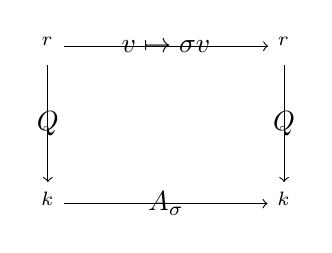
\begin{tikzpicture}
		\node (lt) {$\rational^r$};
		\node (rt) at (3,0) {$\rational^r$};
		\node (lb) at (0,-2) {$\rational^k$};
		\node (rb) at (3,-2) {$\rational^k$};
		\draw[->] (lt) to node {$v\mapsto \sigma v$} (rt);
		\draw[->] (lb) to node {$A_\sigma$} (rb);
		\draw[->] (lt) to node [swap] {$Q$} (lb);
		\draw[->] (rt) to node {$Q$} (rb);
		\end{tikzpicture}
	\end{center}
	commutes. Hence, the group action of $\mathcal{S}$ on $\rational^r$ induces a group action of $\mathcal{S}$ on $\rational^k$ with $(\sigma,v) \mapsto A_\sigma v$, such that the map defined by $Q$ becomes equivariant.
	
	We define $A_\sigma$ as follows: For $i\in\{1,\dots,k\}$, choose $v_i\in\rational^r$ such that $Q v_i = e_i\in\rational^k$. Then the $i$\=/th column of $A_\sigma$ is given by $Q(\sigma v_i)$. By construction, the diagram commutes on the subspace $T\subseteq\rational^r$ with basis $\{v_1,\dots,v_k\}$. It also commutes on $\ker(Q)$, sending all $v\in\ker(Q)$ to $0$ due to $\sigma v\in\ker(Q)$. We conclude that the diagram commutes on all $\rational^r = \ker(Q) \oplus T$.
	
	Since we have
	$$\Im(A_\sigma) = Q(\sigma\rational^r) = Q(\rational^r) = k,$$
	$A_\sigma$ is invertible.
\end{remark}

\begin{lemma}[\phantom{}{\cite[Lemma 4.7]{gitfan_symmetry}}]
	\label{lemma:symmetry_group_on_afaces}
	The action $\mathcal{S}\acts\rational^r$ induces an action of $\mathcal{S}$ on the set of \afaces{}.
\end{lemma}
\begin{proof}
	Let $\sigma\in\mathcal{S}$ and $\gamma_0\preceq\gamma$. We have to show that $\sigma\gamma_0$ is again an \aface{}. Since $\mathcal{S}$ permutes the canonical unit vectors, $\sigma\gamma_0$ is a face of $\gamma$. Let $x\in X\cap \T_{\gamma_0}$. We define $z\in\field^r$ such that
	$$z_i = c_{\sigma^{-1},i} \cdot x_{\sigma^{-1}(i)}\quad\forall 1\leq i \leq r$$
	with $c_{\sigma^{-1}}$ as in Definition~\ref{definition:symmetry_group}. It holds that
	$$
	e_i\in\sigma\gamma_0
	\ \Leftrightarrow\ e_{\sigma^{-1}(i)}\in\gamma_0
	\ \Leftrightarrow\ x_{\sigma^{-1}(i)} \neq 0
	\ \Leftrightarrow\ z_i = c_{\sigma^{-1},i} \cdot x_{\sigma^{-1}(i)} \neq 0
	\quad\forall 1\leq i\leq r,
	$$
	implying $z\in\T_{\sigma\gamma_0}$. Let $f\in\ideal$. By construction, we have $f(z) = (\sigma^{-1}f)(x)$. Now, $\sigma^{-1}f\in\ideal$ and $x$ vanishes on $\ideal$, so that $f(z) = 0$. For this reason $z\in X = V(\ideal)$ holds and $\sigma\gamma_0$ is an \aface{}.
\end{proof}

\begin{prop}
	\label{proposition:symmetry_group_on_orbit_cones}
	The action $\mathcal{S}\acts\rational^k$ introduced in Remark~\ref{remark:symmetry_group_on_image} induces an action $\mathcal{S}\acts\Omega_\ideal^{(k)}$. In particular, $\mathcal{S}$ acts on $\Sigma_T(X)^{(k)}$.
\end{prop}
\begin{proof}
	Let $\sigma\in\mathcal{S}$ and $Q(\gamma_0)\in\Omega_\ideal$ with $\gamma_0\preceq\gamma$ being an \aface{}. We show that $\sigma Q(\gamma_0)\in\Omega_\ideal^{(k)}$. By Remark~\ref{remark:symmetry_group_on_image}, $Q$ is equivariant. It follows that $\sigma Q(\gamma_0) = Q(\sigma\gamma_0)$. Since $\sigma\gamma_0$ is an \aface{} by Lemma~\ref{lemma:symmetry_group_on_afaces}, we have $\sigma Q(\gamma_0)\in\Omega_\ideal$.
	
	If $\lambda(p)$ is a GIT cone, then $\sigma \lambda(p)$ is the GIT cone associated to $A_\sigma p$, as it holds that
	$$A_\sigma p \in A_\sigma \vartheta = \sigma \vartheta \ \Leftrightarrow\ p\in \vartheta\quad \forall \vartheta\in\Omega_\ideal.$$
	Hence, $\mathcal{S}$ also acts on $\Sigma_T(X)$.
	
	Note that the action of $\mathcal{S}$ on cones in $\rational^k$ preserves dimensions because the matrices $A_\sigma$ are invertible. Consequently, we can restrict the actions on $\Omega_\ideal$ and $\Sigma_T(X)$ to cones of the fixed dimension $k$.
\end{proof}

Later on in chapter~\ref{chapter:moduli_space_of_pointed_stable_curves}, we are going to intersect the GIT fan with the cone of movable divisor classes of a Mori dream space. If this cone is invariant under the action of $\mathcal{S}$ on $\rational^k$, it suffices to intersect it with a representative system of orbit cone orbits only. The following proposition together with Remark~\ref{remark:cone_of_divisor_classes_in_mn_context} states the cone's invariance. 

\begin{prop}
	\label{prop:invariance_moving_cone}
	The convex cone
	$$\bigcap_{\gamma_0 \preceq \gamma\ \mathrm{facet}} Q(\gamma_0)\subseteq \rational^k$$
	is invariant with respect to the action $\mathcal{S}\acts \rational^k$.
\end{prop}
\begin{proof}
	Let $\sigma\in\mathcal{S}$. Since permutations in $\mathcal{S}_r$ permute the subsets of $\{1,\dots,r\}$ with cardinality $r-1$, the facets of $\gamma$ are permuted by $\sigma$. It follows that
	$$\sigma\cdot\left(\bigcap_{\gamma_0 \preceq \gamma\ \mathrm{facet}} Q(\gamma_0) \right)
	= \bigcap_{\gamma_0 \preceq \gamma\ \mathrm{facet}} \sigma\cdot Q(\gamma_0)
	= \bigcap_{\gamma_0 \preceq \gamma\ \mathrm{facet}} Q(\sigma \gamma_0)
	= \bigcap_{\gamma_0 \preceq \gamma\ \mathrm{facet}} Q(\gamma_0).$$
\end{proof}

Taking the symmetry group $\mathcal{S}$ into account, it suffices to traverse the following graph in order to determine the GIT fan.

\begin{defi}
	The graph $\mathcal{G}_\mathcal{S}(\Sigma_T(X))$ is the undirected graph with nodes in
	$$\faktor{\Sigma_T(X)^{(k)}}{\mathcal{S}}$$ 
	and the symmetric relation
	$$E_{\mathcal{G}_\mathcal{S}(\Sigma_T(X))} \defeq \left\{\{\mathcal{S}\lambda, \mathcal{S}\mu\}\ \middle|\ \{\lambda, \mu\} \in  E_{\mathcal{G}(\Sigma_T(X))}\right\}.$$
	\index{GSSigmaTX@$\mathcal{G}_\mathcal{S}(\Sigma_T(X))$}%
	\index{EGSSigmaTX@$E_{\mathcal{G}_\mathcal{S}(\Sigma_T(X))}$}%
\end{defi}

\begin{remark}
	Since $\mathcal{G}(\Sigma_T(X))$ is connected, it follows that the graph $\mathcal{G}_\mathcal{S}(\Sigma_T(X))$ is connected.
\end{remark}

\begin{algorithm}
	\caption{Computing all neighbours of a GIT cone orbit}
	\label{algo:git_cone_orbit_neighbours}
	
	\KwIn{A GIT cone orbit $\O\in\faktor{\Sigma_T(X)^{(k)}}{\mathcal{S}}$}
	\KwOut{All GIT cone orbits $\O_\mathcal{N}\in\faktor{\Sigma_T(X)^{(k)}}{\mathcal{S}}$ such that $\{\O, \O_\mathcal{N}\}\in E_{\mathcal{G}_\mathcal{S}(\Sigma_T(X))}$}
	\BlankLine
	$\mathcal{N} \leftarrow \emptyset$\;
	Choose $\lambda$ such that $\O = \mathcal{S}\lambda$\;
	\For(\Comment*[f]{by Algorithm~\ref{algo:compute_git_cone_neighbours}}){$\mu$ such that $\{\lambda,\mu\}\in E_{\mathcal{G}(\Sigma_T(X))}$\label{algo_line:git_cone_orbit_neighbours_loop}}{
		$\mathcal{N}\leftarrow \mathcal{N} \cup \{\mathcal{S}\mu\}$\;
	}
	\Return $\mathcal{N}$\;
\end{algorithm}

\begin{prop}
	Algorithm~\ref{algo:git_cone_orbit_neighbours} computes all neighbours of a node in $\mathcal{G}_\mathcal{S}(\Sigma_T(X))$.
\end{prop}
\begin{proof}
	We reuse the notation of Algorithm~\ref{algo:git_cone_orbit_neighbours}. Clearly, for all  $\O_\mathcal{N}\in\mathcal{N}$ it holds that $\{\O,\O_\mathcal{N}\}\in E_{\mathcal{G}_\mathcal{S}(\Sigma_T(X))}$.
	
	Conversely, let $\O_\mathcal{N}\in\Sigma_T(X)^{(k)}/\mathcal{S}$ such that $\{\O,\O_\mathcal{N}\}\in E_{\mathcal{G}_\mathcal{S}(\Sigma_T(X))}$. Then there exist $\lambda',\mu'\in\Sigma_T(X)^{(k)}$ such that $\{\lambda', \mu'\}\in E_{\mathcal{G}(\Sigma_T(X))}$ and $\O = \mathcal{S}\lambda'$, $\O_\mathcal{N} = \mathcal{S}\mu'$. Let $\sigma\in\mathcal{S}$ such that $\lambda' = \sigma\lambda$. Let $\vartheta$ be the common facet of $\lambda'$ and $\mu'$ and $n_{\lambda'}$, $n_{\mu'}$ the corresponding inner\=/pointing normals. Then $\sigma^{-1}\vartheta$ is the common facet of $\sigma^{-1}\lambda'$ and $\sigma^{-1}\mu'$ with inner\=/pointing normals $(A_{\sigma^{-1}}^*)^{-1} n_{\lambda'}$ and $(A_{\sigma^{-1}}^*)^{-1} n_{\mu'}$, where $A_{\sigma^{-1}}^*$ is the classical adjoint of $A_{\sigma^{-1}}$. In particular, $\{\lambda, \sigma^{-1}\mu'\}\in E_{\mathcal{G}(\Sigma_T(X))}$. Due to $\O = \mathcal{S}\lambda$ and $\O_\mathcal{N} = \mathcal{S}\mu' = \mathcal{S}(\sigma^{-1}\mu')$, it follows that $\O_\mathcal{N}$ is added to $\mathcal{N}$ when iterating the loop in Line~\ref{algo_line:git_cone_orbit_neighbours_loop}.
\end{proof}

Finally, Algorithm~\ref{algo:compute_git_cone_orbits} computes all full dimensional GIT cone orbits. It arises from Algorithm~\ref{algo:compute_git_cones} by small modifications coloured in red.

\begin{algorithm}
	\caption{Computing all full dimensional GIT cone orbits}
	\label{algo:compute_git_cone_orbits}
	
	\KwIn{$Q(\gamma),\ \Omega_\ideal^{(k)}$}
	\KwOut{$\textcolor{red}{\faktor{\textcolor{black}{\Sigma_T(X)^{(k)}}}{\mathcal{S}}}$}
	\BlankLine
	\Repeat{$\dim(\lambda(p)) = k$}{
		Choose random point $p\in Q(\gamma)$\;
	}
	$\mathcal{C} \leftarrow \{\textcolor{red}{\mathcal{S}}\lambda(p)\}$\;
	$\mathcal{F} \leftarrow \{\textcolor{red}{\mathcal{S}}\lambda(p)\}$\;
	\While{$\mathcal{F}\neq \emptyset$}{
		Choose $\textcolor{red}{\O}\in\mathcal{F}$\;
		$\mathcal{F} \leftarrow \mathcal{F} \setminus \{\textcolor{red}{\O}\}$\;
		\For(\Comment*[f]{by Algorithm~\textcolor{red}{\ref{algo:git_cone_orbit_neighbours}}}){$\textcolor{red}{\O_\mathcal{N}}$ with $\{\textcolor{red}{\O,\O_\mathcal{N}}\}\in E_{\mathcal{G}_{\textcolor{red}{\mathcal{S}}}(\Sigma_T(X))}$}{
			\If{$\textcolor{red}{\O_\mathcal{N}}\notin\mathcal{C}$}{
				$\mathcal{C} \leftarrow \mathcal{C} \cup \{\textcolor{red}{\O_\mathcal{N}}\}$\;
				$\mathcal{F} \leftarrow \mathcal{F} \cup \{\textcolor{red}{\O_\mathcal{N}}\}$\;
			}
		}
	}
	\Return $\mathcal{C}$\;
\end{algorithm}

\section{Counterexample: Removal of non-minimal orbit cones}

By discarding as many orbit cones as possible in $\Omega_\ideal^{(k)}$ without affecting the resultant GIT fan, one can speed up the computation of the associated GIT cone $\lambda(p)$ of an arbitrary point $p\in Q(\gamma)$. Clearly, one can discard all orbit cones being a union or intersection of the remaining ones. However, the approach in \cite{gitfan_symmetry} of removing all non\=/minimal cones in $\Omega_\ideal^{(k)}$ with respect to inclusion is flawed. Fortunately, \cite[Theorem 1.1]{gitfan_symmetry} still holds as all non-minimal orbit cones are unions of minimal ones for the \msix{} example.

Consider the following scenario. Let $f = x_1x_3+x_2x_4+x_5\in \field[x_1,x_2,x_3,x_4,x_5]$. Set  $\ideal := \langle x_3, x_4\rangle \cdot \langle f\rangle$ and
$$Q = (q_1, q_2, q_3, q_4, q_5) := \begin{pmatrix}
0 & 0 & 1 & 1 & 1 \\
1 & 0 & 0 & 1 & 1 \\
1 & 1 & 1 & 1 & 2 
\end{pmatrix}.$$

It is easy to see that the matrix $Q$ is of full rank 3 and that $f$ and thus $\ideal$ are homogeneous with respect to the $\integer^3$\=/grading induced by $Q$. Furthermore, $\ideal$ does not contain any monomials. Overall, $\ideal$ and $Q$ constitute a valid setup in the sense of section~\ref{section:setup}. The $\ideal$-faces with full dimensional image in $Q(\gamma)$ are given by
\begin{align*}
\gamma_1 &:=\langle e_1, e_2, e_5\rangle \\
\gamma_2 &:=\langle e_1, e_2, e_3, e_5\rangle \\
\gamma_3 &:=\langle e_1, e_2, e_4, e_5\rangle \\
\gamma_4 &:=\langle e_1, e_3, e_4, e_5\rangle \\
\gamma_5 &:=\langle e_2, e_3, e_4, e_5\rangle \\
\gamma_6 &:=\langle e_1, e_2, e_3, e_4\rangle \\
\gamma_7 &:=\langle e_1, e_2, e_3, e_4, e_5\rangle
\end{align*}
and may be computed manually by taking all faces $\gamma_0\preceq \gamma$ with dimension $\geq 3$ and identifying those such that $\ideal_{\gamma_0}$ does not contain a monomial.

The orbit cones $Q(\gamma_j)\in \rational^3_{z_1,z_2,z_3}$ yield the following polytopes when intersecting them with the $\{z_3 = 1\}$\=/plain:

\psset{xunit=2cm,yunit=2cm}
\begin{minipage}{.325\textwidth}\centering
	\begin{pspicture}(-0.5, -0.5)(1.25, 1.25)
	\psaxes{->}(0,0)(1.25,1.25)
	\psgrid[griddots=20,subgriddots=10,subgriddiv=2,gridlabels=0pt](2,2)
	\pspolygon[fillstyle=solid,fillcolor=red,opacity=0.4](0,1)(0,0)(0.5,0.5)
	\rput(0.6,0.75){$Q(\gamma_1)$}
	\end{pspicture}
\end{minipage}
\begin{minipage}{.325\textwidth}\centering
	\begin{pspicture}(-0.5, -0.5)(1.25, 1.25)
	\psaxes{->}(0,0)(1.25,1.25)
	\psgrid[griddots=20,subgriddots=10,subgriddiv=2,gridlabels=0pt](2,2)
	\pspolygon[fillstyle=solid,fillcolor=orange,opacity=0.4](0,1)(0,0)(1,0)
	\rput(0.35,0.25){$Q(\gamma_2)$}
	\end{pspicture}
\end{minipage}
\begin{minipage}{.325\textwidth}\centering
	\begin{pspicture}(-0.5, -0.5)(1.25, 1.25)
	\psaxes{->}(0,0)(1.25,1.25)
	\psgrid[griddots=20,subgriddots=10,subgriddiv=2,gridlabels=0pt](2,2)
	\pspolygon[fillstyle=solid,fillcolor=orange,opacity=0.4](0,1)(0,0)(1,1)
	\rput(0.35,0.7){$Q(\gamma_3)$}
	\end{pspicture}
\end{minipage}
\begin{minipage}{.325\textwidth}\centering
	\begin{pspicture}(-0.5, -0.5)(1.25, 1.25)
	\psaxes{->}(0,0)(1.25,1.25)
	\psgrid[griddots=20,subgriddots=10,subgriddiv=2,gridlabels=0pt](2,2)
	\pspolygon[fillstyle=solid,fillcolor=red,opacity=0.4](0,1)(1,0)(1,1)
	\rput(0.65,0.7){$Q(\gamma_4)$}
	\end{pspicture}
\end{minipage}
\begin{minipage}{.325\textwidth}\centering
	\begin{pspicture}(-0.5, -0.5)(1.25, 1.25)
	\psaxes{->}(0,0)(1.25,1.25)
	\psgrid[griddots=20,subgriddots=10,subgriddiv=2,gridlabels=0pt](2,2)
	\pspolygon[fillstyle=solid,fillcolor=red,opacity=0.4](0,0)(1,0)(1,1)
	\rput(0.65,0.25){$Q(\gamma_5)$}
	\end{pspicture}
\end{minipage}
\begin{minipage}{.325\textwidth}\centering
	\begin{pspicture}(-0.5, -0.5)(1.25, 1.25)
	\psaxes{->}(0,0)(1.25,1.25)
	\psgrid[griddots=20,subgriddots=10,subgriddiv=2,gridlabels=0pt](2,2)
	\pspolygon[fillstyle=solid,fillcolor=orange,opacity=0.4](0,0)(0,1)(1,1)(1,0)
	\rput(0.5,0.66){$Q(\gamma_6)$}
	\rput(0.5,0.33){$Q(\gamma_7)$}
	\end{pspicture}
\end{minipage}

When taking all orbit cones into account, the intersection of the resultant GIT fan and the $\{z_3 = 1\}$\=/plain yields

\begin{center}
	\begin{pspicture}(-0.5, -0.5)(1.25, 1.25)
	\psaxes{->}(0,0)(1.25,1.25)
	\psgrid[griddots=20,subgriddots=10,subgriddiv=2,gridlabels=0pt](2,2)
	\pspolygon[fillstyle=solid,fillcolor=orange,opacity=0.4](0,0)(0,1)(1,1)(1,0)
	\psline(1,0)(0,1)
	\psline(0,0)(1,1)
	\end{pspicture}
\end{center}

However, when considering only the red orbit cones, which are minimal with respect to inclusion, all full dimensional intersections of orbit cones containing a common point -- that is maximal GIT cones -- have the following form when intersecting them with the $\{z_3 = 1\}$\=/plain:

\begin{minipage}{.245\textwidth}\centering
	\begin{pspicture}(-0.5, -0.5)(1.25, 1.25)
	\psaxes{->}(0,0)(1.25,1.25)
	\psgrid[griddots=20,subgriddots=10,subgriddiv=2,gridlabels=0pt](2,2)
	\pspolygon[fillstyle=solid,fillcolor=orange,opacity=0.4](0,1)(0,0)(0.5,0.5)
	\end{pspicture}
\end{minipage}
\begin{minipage}{.245\textwidth}\centering
	\begin{pspicture}(-0.5, -0.5)(1.25, 1.25)
	\psaxes{->}(0,0)(1.25,1.25)
	\psgrid[griddots=20,subgriddots=10,subgriddiv=2,gridlabels=0pt](2,2)
	\pspolygon[fillstyle=solid,fillcolor=orange,opacity=0.4](1,1)(1,0)(0.5,0.5)
	\end{pspicture}
\end{minipage}
\begin{minipage}{.245\textwidth}\centering
	\begin{pspicture}(-0.5, -0.5)(1.25, 1.25)
	\psaxes{->}(0,0)(1.25,1.25)
	\psgrid[griddots=20,subgriddots=10,subgriddiv=2,gridlabels=0pt](2,2)
	\pspolygon[fillstyle=solid,fillcolor=orange,opacity=0.4](0,1)(1,0)(1,1)
	\end{pspicture}
\end{minipage}
\begin{minipage}{.245\textwidth}\centering
	\begin{pspicture}(-0.5, -0.5)(1.25, 1.25)
	\psaxes{->}(0,0)(1.25,1.25)
	\psgrid[griddots=20,subgriddots=10,subgriddiv=2,gridlabels=0pt](2,2)
	\pspolygon[fillstyle=solid,fillcolor=orange,opacity=0.4](0,0)(1,0)(1,1)
	\end{pspicture}
\end{minipage}

It is evident that these cannot constitute the maximal cones of a fan. Most of all, we are not able to recover the GIT fan. Note that $Q(\gamma_1)$, $Q(\gamma_6)$ and $Q(\gamma_7)$ are the only orbit cones that may be discarded. They are either the union or intersection of a subset of $Q(\gamma_2),\dots, Q(\gamma_5)$.


	\chapter{Implementation}

In the following we present the implementation of the algorithm discussed in the previous chapter. In contrast to the existing \singular{} implementation \gitfanlib{} \cite{gitfanlib}, which forms the foundation of our work, the approach described here utilises high performance computing methods in order to speed up the execution by running the algorithm on any number of machines simultaneously. Naturally, one has to identify independent components permitting concurrent execution on the one hand and inherent sequential processes on the other hand. As the sequential components of the algorithm mostly agree with \gitfanlib{}, we discuss only reworked parts and skip the remaining ones, referring the interested reader to \cite{gitfanlib}. The chapter is structured as follows: First, we discuss the employed parallelisation framework \gpispace{} developed by the \ac{Fraunhofer ITWM} and follow up with the integration of singular code into \gpispace{} applications. After encoding GIT cone orbits, we present a parallel design of Algorithm~\ref{algorithm:main} that is applicable for any kind of fan traversals. Finally, we describe input and output formats, additional features such as speeding up the execution by precomputed results, and executed software tests in order to verify the functional correctness of the program.

\section{\gpispace}

\gpispace{} is a workflow management system developed by the \ac{Fraunhofer ITWM} which supports the execution of arbitrary workflows on ultra scale systems \cite{gpispace}. It consists of three key components: 
\begin{itemize}
	\item the \ac{DRTS}, which is responsible for building and managing arbitrary worker topologies based on the available compute nodes, resource management and job scheduling. It supports the reallocation of jobs in case of hardware failures and further integrates dynamically added hardware
	\item the \ac{WE}. It tracks the state of the workflow, identifies a front of activities for which all dependencies are resolved and laces jobs from input data and active transitions which then are sent to the \ac{DRTS} for scheduling.
	\item a virtual memory layer, which provides the necessary infrastructure for the \ac{PGAS} programming model. It relies on \textsc{GPI} by \ac{Fraunhofer ITWM} \cite{gpi}.
\end{itemize}

The framework has been developed with separation of concerns in mind, whereby the concerns here are given by computation and coordination \cite{coordination_language}. In our case the computation takes place in sequential \singular-routines. The dependencies and data transfers between this routines, which assemble the particular routines into a complex, parallel algorithm, are described by a special domain language in the the coordination layer. In \gpispace{}, this domain language is chosen to be an extension of the well known Petri net model introduced in 1962 by Carl Adam Petri \cite{petri}. Its formal nature permits a vast range of analysis and verification techniques. Concurrency is easily described due to locality of states. Furthermore, Petri nets yield precise execution semantics, supporting interruptions and restarts by differentiating between activation and execution of functional units. For this reason, fault tolerance to hardware failures is achieved by simply restarting failed executions. \cite{petri_net_wms}

\gpispace{} is shipped with an appropriate compiler that generates all files which are necessary for execution from a XML description of a given Petri net. Furthermore, \gpispace{} also provides a basic visualization tool that comes in handy when debugging small to medium sized nets.

\subsection*{Petri nets}

Formally, an (unweighted) \emph{Petri net} is a triple $(P, T, F)$ of \emph{places} $P$, \emph{transitions} $T$ and directed \emph{arcs} $F\subseteq (P\times T)\cup(T\times P)$ relating the former concepts. We demand that $P\cap T = \emptyset$. A function $M\colon P\rightarrow\natural$ is called \emph{marking} and describes a possible state of the Petri net. If we have $M(p)=k$ for a place $p$ and the current state of the Petri net is given by $M$, we say that $p$ holds $k$ \emph{tokens}. Visually, circles depict places, rectangles are transitions and arrows between circles and rectangles represent arcs whose direction is indicated by the tip. The current state $M$ of the Petri net is displayed by placing $M(p)$ dots in the circle representing the place $p$. Figure~\ref{net:sample} gives an example for the graphical representation of a Petri net.

\begin{figure}
	\centering
	\begin{tikzpicture}
	\node[place,tokens=2] (0) {};
	\node[transition] (1) [right of=0] {};
	\node[place]      (2) [right of=1] {};
	\path
		(0) edge [post] (1)
		(1) edge [post] (2);
	\end{tikzpicture}
	\caption{Graphical representation of a Petri net with two places and one transition. The current state is a marking that sends the left place to $2$ and the second place to $0$.}
	\label{net:sample}
\end{figure}

A transition $t$ is said to be \emph{active}, iff
$$\forall p\in P\colon (p,t)\in F\Rightarrow M(p) > 0$$
holds. In this case \emph{firing} $t$ means to transform the current state $M$ into $M'$ by the update rule
$$M'(p) \defeq \begin{cases}
M(p) - 1 & (p,t)\in F,\ (t,p)\notin F \\
M(p) + 1 & (p,t)\notin F,\ (t,p)\in F \\
M(p) & \text{else}
\end{cases}$$
for all $p\in P$. We interpret this as follows: For every incoming arc $(p,t)$ from $p$ a token in $p$ is consumed and for every outgoing arc $(t, p')$ to $p'$ a new token is placed into $p'$. Note that the notion of tokens ``moving through transitions'' instead of consumption and creation of tokens is erroneous as we will see later on when attaching data to them.

\begin{figure}
	\centering
	\begin{tikzpicture}
	\node[place,tokens=1] (0) {};
	\node[transition] (1) [right of=0] {};
	\node[place]      (2) [right of=1] {};
	\path
		(0) edge [post] (1)
		(1) edge [post] (2);
		
	\node[place,tokens=1] (3) [below of =0] {};
	\node[transition] (4) [right of=3] {};
	\node[place]      (5) [right of=4] {};
	\path
	(3) edge [post] (4)
	(4) edge [post] (5);
	\end{tikzpicture}
	\caption{Modelling concurrent processes in a Petri net.}
	\label{net:sample_concurrency}
\end{figure}

An important property of Petri nets is given by the fact that in many cases the same result is obtained if the order in which two transitions $t_1$ and $t_2$ fire is reversed. This allows the modelling of concurrent behaviour. When executing the Petri net model on a machine, the necessary steps for firing $t_1$ and $t_2$ respectively may be performed in parallel. Figure~\ref{net:sample_concurrency} depicts such a situation. Note that Figure~\ref{net:sample} also shows an example for concurrent behaviour in which the transition may fire twice. However, the order in which the tokens in the left place are consumed is of no relevance. This example seems trivial as tokens located at the same place are indistinguishable. However, this is not the case anymore when attaching data to tokens. In fact, Figure~\ref{net:sample} depicts the common scenario of concurrent behaviour in our algorithm, as parallel execution is mostly achieved by invoking the same routine for varying, independent input data.

\subsection*{Coloured Petri nets and guards}

Workflows describe a (possible concurrent) progression of processes, hence it is evident to model a process by a transition. The input and output data of a process is taken into account by attaching data values of a predefined type to each token. Then every incoming arc provides input data for the process corresponding to the target transition, whereas every outgoing arc describes output data of the source transition that should be put into the target place. A place may only hold tokens of a single type, introducing strong typing to Petri nets. This kind of Petri net is called \emph{coloured Petri net}, developed by Kurt Jensen in 1980. The term originates from the analogy of understanding each distinct type as a unique color. A formal treatment of this concept may be found in \cite{cp_nets}.

In order to control the data flow, each transition may be tagged with a predicate over the types of places with incoming arcs, which is called \emph{condition} or \emph{guard} \cite{cp_nets}. The activation rule for a transition is extended such that not only a token has to be present for every incoming arc, but also the data values of the consumed tokens have to satisfy the condition. \gpispace{} provides its own expression language in order to specify conditions. Figure~\ref{net:sample_guard} shows a transition that consumes tokens with positive data values only.

\begin{figure}
	\centering
	\begin{tikzpicture}
	\node[place,tokens=2] (0) {};
	\node[transition] (1) [right of=0] {};
	\path
		(0) edge [post] (1);
	\node[anchor=west] at ($(0) + (-1.8,0)$) {$\begin{aligned}x &= 1\\[-3\jot] x&= -1\end{aligned}$};
	\node at ($(1) + (0,0.7)$) {$\gpiresolve{x} \gpigt 0$};
	\end{tikzpicture}
	\caption{Guards in a Petri net. Only the token with $x=1$ activates the transition.}
	\label{net:sample_guard}
\end{figure}

\subsection*{Expressions}

\gpispace{} supports two kinds of transitions. The first kind triggers a module call whenever firing, executing arbitrary \cplusplus code where the input and output tokens are mapped to references. The module call is packaged as a job and scheduled by the \ac{DRTS}. A lightweight approach that requires no scheduling is given by the second kind of transition. The expression language provided by \gpispace{} allows to specify the output data values of a transition by means of simple operations on the input data values. This extension is intended to be used for minor computations and saves the overhead of generating and scheduling a job by executing the expression directly within the \ac{WE}. For instance, counting consumed tokens may be realised that way, see Figure~\ref{net:sample_expression}. If the counting would be realised with \cplusplus, each increment will cause a disproportionate communication and scheduling overhead.

\begin{figure}[t]
	\centering
	\begin{tikzpicture}
	\node[place,tokens=3] (0) {};
	\node[transition] (1) [right of=0] {};
	\node[place,tokens=1] (2) [right of=1] {};
	\path
		(0) edge [post] (1)
		(2) edge [pre, bend right] (1)
		(2) edge [post, bend left] (1);
	\node[draw] at ($(1) + (0,-0.9)$) {$\gpiresolve{i} \defeq \gpiresolve{i} + 1$};
	\node at ($(2) + (1,0)$) {$i = 0$};
	\end{tikzpicture}
	\caption{Expressions in a Petri net. After firing the transition three times, the left place contains no tokens anymore and the right place contains one token with $i=3$.}
	\label{net:sample_expression}
\end{figure}

\subsection*{Executing Petri nets}

The \ac{WE} is responsible for executing a given Petri net. It manages its current state and identifies active transitions. Whenever such a transition is detected, its input tokens are consumed, bundling the attached data values into a job that describes the execution of the transition. Then, this job is submitted to the \ac{DRTS} where it awaits its execution. The set of active transitions not being executed already is called front of activities and generally contains numerous elements at once due to the locality of Petri nets. Thus, the \ac{DRTS} is able to utilise the available capacities by scheduling multiple jobs in parallel.

When a job finishes, the results are returned to the \ac{WE} which extracts the output tokens and updates the state of the Petri net accordingly. Note that during the whole process described above, the input tokens for an active transition are consumed whereas the output tokens are not available yet. In order to fully describe the state of an executable Petri net, one has to incorporate the knowledge about all active transitions and its cached tokens into the state description. Hence, the \ac{WE} has to manage \emph{timed}, coloured Petri nets. Figure~\ref{net:sample_execution} illustrates the process of executing two active transitions in parallel. The module called by the transition sleeps for $x$ seconds, where $x$ is the input data value, and then returns the increment $x + 1$.

\begin{figure}[t]
	\centering
	\begin{tabular}{cc}
		\adjustbox{valign=t}{\begin{tikzpicture}[framed]
		\node[place,tokens=2] (0) {};
		\node[transition] (1) [right of=0] {};
		\node[place]      (2) [right of=1] {};
		\path
		(0) edge [post] (1)
		(1) edge [post] (2);
		\node[anchor=west] at ($(0) + (-1.6,0)$) {$\begin{aligned}x &= 1\\[-3\jot] x&= 5\end{aligned}$};
		\node[anchor=west] at ($(2) + (0.4,0)$) {\phantom{$x = 1$}};
		
		\node[anchor=west,inner sep=0] at ($(0.west) + (0,-0.8)$) {active transitions:};
		\end{tikzpicture}}
		&
		\adjustbox{valign=t}{\begin{tikzpicture}[framed]
		\node[place,tokens=1] (0) {};
		\node[transition] (1) [right of=0] {};
		\node[place]      (2) [right of=1] {};
		\path
		(0) edge [post] (1)
		(1) edge [post] (2);
		\node[anchor=west] at ($(0) + (-1.6,0)$) {$x = 1$};
		\node[anchor=west] at ($(2) + (0.4,0)$) {\phantom{$x = 1$}};
		
		\node[anchor=west,inner sep=0] at ($(0.west) + (0,-0.8)$) {active transitions:};
		\node[place,tokens=1] (0') at ($(0) + (0,-1.6)$) {};
		\node[transition] (1') [right of=0'] {};
		\node[place]      (2') [right of=1'] {};
		\path
		(0') edge [post] (1')
		(1') edge [post] (2');
		\node[anchor=west] at ($(0') + (-1.6,0)$) {$x = 5$};
		\end{tikzpicture}}
		\\[2.5cm]
		\adjustbox{valign=t}{\begin{tikzpicture}[framed]
		\node[place] (0) {};
		\node[transition] (1) [right of=0] {};
		\node[place]      (2) [right of=1] {};
		\path
		(0) edge [post] (1)
		(1) edge [post] (2);
		\node[anchor=west] at ($(0) + (-1.6,0)$) {\phantom{$x = 1$}};
		\node[anchor=west] at ($(2) + (0.4,0)$) {\phantom{$x = 1$}};
		
		\node[anchor=west,inner sep=0] at ($(0.west) + (0,-0.8)$) {active transitions:};
		\node[place,tokens=1] (0') at ($(0) + (0,-1.6)$) {};
		\node[transition] (1') [right of=0'] {};
		\node[place]      (2') [right of=1'] {};
		\path
		(0') edge [post] (1')
		(1') edge [post] (2');
		\node[anchor=west] at ($(0') + (-1.6,0)$) {$x = 5$};
		\node[place,tokens=1] (0'') [below of=0'] {};
		\node[transition] (1'') [right of=0''] {};
		\node[place]      (2'') [right of=1''] {};
		\path
		(0'') edge [post] (1'')
		(1'') edge [post] (2'');
		\node[anchor=west] at ($(0'') + (-1.6,0)$) {$x = 1$};
		\end{tikzpicture}}
		&
		\adjustbox{valign=t}{\begin{tikzpicture}[framed]
		\node[place] (0) {};
		\node[transition] (1) [right of=0] {};
		\node[place,tokens=1] (2) [right of=1] {};
		\path
		(0) edge [post] (1)
		(1) edge [post] (2);
		\node[anchor=west] at ($(0) + (-1.6,0)$) {\phantom{$x = 1$}};
		\node[anchor=west] at ($(2) + (0.4,0)$) {$x = 2$};
			
		\node[anchor=west,inner sep=0] at ($(0.west) + (0,-0.8)$) {active transitions:};
		\node[place,tokens=1] (0') at ($(0) + (0,-1.6)$) {};
		\node[transition] (1') [right of=0'] {};
		\node[place]      (2') [right of=1'] {};
		\path
		(0') edge [post] (1')
		(1') edge [post] (2');
		\node[anchor=west] at ($(0') + (-1.6,0)$) {$x = 5$};
		\end{tikzpicture}}
		\\[3.8cm]
		\adjustbox{valign=t}{\begin{tikzpicture}[framed]
		\node[place] (0) {};
		\node[transition] (1) [right of=0] {};
		\node[place,tokens=2] (2) [right of=1] {};
		\path
		(0) edge [post] (1)
		(1) edge [post] (2);
		\node[anchor=west] at ($(0) + (-1.6,0)$) {\phantom{$x = 1$}};
		\node[anchor=west] at ($(2) + (0.4,0)$) {$\begin{aligned}x &= 2\\[-3\jot] x&= 6\end{aligned}$};
		
		\node[anchor=west,inner sep=0] at ($(0.west) + (0,-0.8)$) {active transitions:};
		\end{tikzpicture}}
		&
		\\
	\end{tabular}
	\caption{Possible execution of a Petri net. The module called by the transition sleeps for $x$ seconds and then returns the increment $x + 1$.}
	\label{net:sample_execution}
\end{figure}

The \ac{WE} itself is executed on a single node of the underlying system. Hence, special care must be taken when designing Petri nets. Instead of firing numerous transitions with execution times of milliseconds, one is advised to aggregate these transitions into a single one with an execution time of several seconds. Otherwise, the \ac{WE} quickly becomes a bottleneck since the amount of scheduled transitions per second does not scale with the number of available computing nodes. Furthermore, the marking of the Petri net is stored in the RAM of a single node. If large quantities of data have to be managed, the tokens should only contain a reasonable amount of metadata pointing to the real data which -- for instance -- is stored in a shared directory.

\gpispace{} assumes that module calls have no side effects. Thus, when implementing the execution code for the transitions, possible racing conditions and concurrency issues have to be considered properly. Furthermore, each worker managed by the \ac{DRTS} is executed in its own process, but beyond that, jobs assigned to the same worker run in the same environment. For this reason jobs are influenced by changes of global state by prior executions. This behaviour causes several issues when integrating \singular{}, which is implemented as a large, global state machine.

\section{Integration of Singular}
\singular{} is a computer algebra system for polynomial computations, with special emphasis on commutative and non\=/commutative, algebraic geometry and singularity theory \cite{singular}. Typically, algorithms utilising \singular{} are written in its own \c\=/like programming language, which is interpreted at runtime. Besides providing a console frontend for code execution, \singular{} also comes with the \c{} library \libsingular{} that implements its full backend. In particular, \c{} methods for interpreting and executing \singular{} code are available. \libsingular{} also exposes the internal data structures used by \singular{}, so that one can write conversion methods between \singular{} types and user defined types, i.e. \gpispace{} types.

Since module calls in \gpispace{} permit the execution of arbitrary \cplusplus{} code, every legacy application with a \c{} interface such as \singular{} can easily be integrated and executed. In order to execute \singular{} code in a module call, one has to perform the following steps:
\begin{enumerate}
	\item Check if a \singular{} instance is already running on the current worker. If not, initialise \singular{}.
	\item Convert \gpispace{} types to \singular{} types.
	\item Map the converted data to identifiers in order to address it by \singular{} code.
	\item Formulate a \c{} string containing the \singular{} code to be executed and pass it to the \singular{} interpreter via \libsingular{}. Note that instead of hard coding large blocks of code, it is reasonable to outsource them into a \singular{} library. Then, this step reduces to loading the library and invoking a single method.
	\item Extract the data mapped to all identifiers that contain results of the computation.
	\item Convert the extracted \singular{} types to \gpispace{} types that can be attached to tokens.
\end{enumerate}

\subsection*{Drawback: Global state}
Although integrating \singular{} code is sufficiently easy, the approach described above suffers from a serious issue that originates from \singular{} heavily relying on global state. For instance, loaded libraries, declared variables and the current basering are managed in global data structures. If module calls are supposed to have no side effects, all changes concerning global state have to be reverted before returning from them. Unfortunately, \libsingular{} lacks the feature of creating and restoring images of its global state. In fact, there seems to be no way of resetting \singular{} to its initial state short of killing the current process, which -- obviously -- is not desirable.

Not being able to reset the \singular{} instance also makes writing decoupled test cases more problematic. In order to avoid tests being influenced by one another due to global \singular{} state, each test has to be executed in a separate process. Unfortunately, this prevents the utilisation of many \gtest{} features such as bundling test cases, reusing data configurations and parametrising tests.

\subsection*{Drawback: No in memory serialization of \singular{} types}
When \gpispace{} has to share \singular{} data between module calls without knowing the internal structure of the data, this can be achieved by serialising the data into \acp{BLOB} which then are managed by the \ac{WE}. \singular{} supports the serialization of its common data types by using \emph{\ac{ssi} file links}. As the name suggests, the serialization string always is written to a file. It would be desirable to also obtain a serialization string in memory without the overhead of using virtual files or reading the created \ac{ssi} files. Currently, we pass metadata (that is file paths) pointing to \ac{ssi} files in a shared directory instead of acquiring and passing \acp{BLOB}.

\subsection*{Drawback: \singular{} programming language lacking data structure implementations}
Since the purpose of developing a parallel implementation of Algorithm~\ref{algorithm:main} is the computation of large examples within a reasonable timeframe, it is crucial to choose optimal data structures for large sets of data. Unfortunately, the \singular{} programming language lacks tree\=/like data structures with $\mathcal{O}(n)$ characteristics and, more importantly, hash tables with average time complexity of $\mathcal{O}(1)$ for insertion, searching and deletion. For this reason, all tasks dealing with the detection of duplicates, were moved from \singular{} into the \cplusplus{} environment, where the \ac{STL} provides all necessary data structure implementations. Hence, the set of found GIT cones is managed in \cplusplus{}. The elimination of duplicates in orbit computations as well as the computation of the symmetry group action on GIT cones have been reworked in \cplusplus{}, resulting in a substantial performance gain compared to the \gitfanlib{} implementation.


\section{Encoding GIT cone orbits}
\label{sec:git_cone_management}
In chapter~\ref{chap:algorithm}, we suggested to traverse a graph that reflects the structure of the maximal cones located in the GIT fan. Since nodes of the graph may be reachable by multiple paths, the traversal algorithm has to manage a list of found nodes such that no node is expanded twice. For this reason it is crucial to develop an encoding of nodes, i.e. GIT cone orbits, that 
\begin{enumerate}[label={\upshape(\roman*)}]
	\item conserves memory, permitting fast bit\=/per\=/bit comparisons,
		\label{enum_item:git_cone_orbit_property_memory}
	\item allows to recover the encoded object from the code word,
		\label{enum_item:git_cone_orbit_property_invertible}
	\item does not require additional effort when computing code words and
		 \label{enum_item:git_cone_orbit_property_computation_effort}
	\item is easily accessible for operations that are frequently performed on the nodes.
		\label{enum_item:git_cone_orbit_property_operations}
\end{enumerate}

We reuse the notation from chapter~\ref{chap:algorithm}. Recall that the matrix $Q\in\field^{k\times r}$ of rank $r$ with columns $q_1,\dots,q_r$ encodes a torus action of a torus $H$ on the affine variety $X = V(\ideal)\subseteq \field^r$ where $\ideal\subseteq \field[x_1,\dots,x_r]$ is a homogeneous ideal with respect to the grading $\deg(x_i) = q_i$, $1\leq i\leq r$. The positive orthant $\rational_{\geq 0}^r$ is denoted by $\gamma$. Furthermore, $\mathcal{S}$ (possibly trivial) denotes a symmetry group of the action of $H$ on $X$.

\subsection*{Encoding GIT cones}
In order to encode GIT cone orbits, we require an appropriate encoding for GIT cones that allows us to apply the group action of $\mathcal{S}$ with minimal costs. The encoding described here originates from \cite[Construction 4.3]{gitfan_symmetry} and has been implemented in \gitfanlib{}. It utilises the result of Lemma~\ref{lemma:git_cones_elementary_properties}, stating that every full dimensional GIT cone is the finite intersection of all full dimensional orbit cones containing the GIT cone. Thus, every GIT cone $\lambda$ can be uniquely identified by bits indexed over $\Omega_\mathfrak{a}^{(k)}$ such that the bit indexed by $\vartheta\in\Omega_\mathfrak{a}^{(k)}$ is set to $1$ iff $\lambda \subseteq \vartheta$. Formally:
$$\code\colon \Lambda(\mathfrak{a},Q)(k) \rightarrow \{0,1\}^{\Omega_\mathfrak{a}^{(k)}},\quad
\lambda \mapsto (b_\vartheta)_{\vartheta\in\Omega_\mathfrak{a}^{(k)}}\quad\text{with}\quad
b_\vartheta = 
\begin{cases}
1, & \vartheta\subseteq\lambda \\
0, & \vartheta\not\subseteq\lambda
\end{cases}\ .
$$
Obviously, this mapping is injective and yields an encoding with code words of length $|\Omega_\mathfrak{a}^{(k)}|$, guaranteeing property \ref{enum_item:git_cone_orbit_property_memory}. The GIT cone is recovered by intersecting all orbit cones indexing a $1$ in the code word. Hence, \ref{enum_item:git_cone_orbit_property_invertible} holds.

Next, we verify property \ref{enum_item:git_cone_orbit_property_computation_effort}. Since every GIT cone $\lambda(p)$ occurring in the algorithm is constructed by taking the relative inner point $p$ and intersecting all orbit cones containing $p$, the code word can be computed alongside the construction of $\lambda(p)$ due to Lemma~\ref{lemma:git_cones_elementary_properties}.

Finally, verifying \ref{enum_item:git_cone_orbit_property_operations},  we have to check that the group action of $\mathcal{S}$ on the code words defined by
$$\sigma\cdot\code(\lambda) \defeq \code(\sigma\cdot\lambda) = \code(A_\sigma\cdot\lambda)$$
is realised by a low\=/cost operation on bit strings. Since we have
$$\lambda\subseteq\vartheta\ \Leftrightarrow\ A_\sigma\cdot\lambda\subseteq A_\sigma\cdot\vartheta,$$ the group action simply permutes the characters of code words in the same way as $\mathcal{S}$ acts on $\Omega_\mathfrak{a}^{(k)}$. We are going to compute the group action $\mathcal{S}\acts\Omega_\mathfrak{a}^{(k)}$ in the next section, so that it is available during the traversal process. Hence, applying a group element to a code word is implemented as the application of a permutation which is stored in a lookup table.

\subsection*{Extending the encoding to orbits}
After encoding GIT cones, we are able to encode GIT cone orbits by mapping each orbit to the code word of an uniquely identified representative. We choose the representative with the minimal code word regarding the lexicographical order over the alphabet $\{0,1\}$. Hence, the encoding is given by
$$\code\colon \faktor{\Lambda(\mathfrak{a},Q)(k)}{\S} \rightarrow \{0,1\}^{\Omega_\mathfrak{a}^{(k)}},\quad
\O \mapsto \min\limits_{\leq_\text{lex}}\ \{\code(\lambda) \mid \lambda\in\O\}$$
and clearly is injective. Property \ref{enum_item:git_cone_orbit_property_memory} is inherited from the GIT cone encoding. The same applies to property \ref{enum_item:git_cone_orbit_property_invertible}, since we already presented an approach for applying group elements to code words, so that we are able to recover the orbit from a single representative. Property \ref{enum_item:git_cone_orbit_property_computation_effort} holds since orbits typically are constructed from a representative and finding the minimal representative is cheap due to property \ref{enum_item:git_cone_orbit_property_operations} of the GIT cone encoding. Finally, since operations on orbits usually are given by well defined operations on their representatives, \ref{enum_item:git_cone_orbit_property_operations} also is inherited from the GIT cone encoding. One simply applies the operation on the GIT cone that is represented by the code word of the orbit.

\section{Application flow \& Concurrency}

We differentiate between three stages when implementing the algorithm described in chapter~\ref{chap:algorithm}. During the first stage, preprocessing of the input data and the identification of all orbits of \afaces{} with full dimensional image takes place. The second stage covers the computation of the orbit cones and the symmetry group action on GIT cone\=/hashes. This data is mandatory when determining the GIT fan in the third stage by traversing all maximal cones of the fan. Figure~\ref{net:algorithm_overview} depicts the simplified data flow of the algorithm in which each stage is collapsed into a single transition. Dashed arcs indicate read-only connections, that is data values of tokens in the source place are passed to the target transition without consuming them when it fires. Hence, \emph{read-only} connections give access to static data computed once (such as processed input data), without discarding it due to consumption.

\begin{figure}[t]
	\centering
	\begin{tikzpicture}
	\node[place] (raw) {raw input};
	\node[transitiontext] (p1) at ($(raw) + (0,-1.5)$) {Stage 1};
	\node[place,anchor=east,minimum width=4cm] (data) at ($(p1) + (-0.5,-1.5)$) {problem data};
	\node[place,anchor=west,minimum width=4cm] (afaces) at ($(p1) + (0.5,-1.5)$) {\afaces};
	\node[transitiontext] (p2) at ($(p1) + (0,-3)$) {Stage 2};
	\node[place,anchor=east,minimum width=4cm] (action) at ($(p2) + (-0.5,-1.5)$) {group action};
	\node[place,anchor=west,minimum width=4cm] (oc) at ($(p2) + (0.5,-1.5)$) {orbit cones};
	\node[transitiontext] (p3) at ($(p2) + (0,-3)$) {Stage 3};
	\node[place] (gc) at ($(p3) + (0,-1.5)$) {GIT cones};
	
	\node[transitiontext,anchor=west] (oc_output) at ($(oc.east) + (1,0)$) {output};
	\node[transitiontext,anchor=west] (gc_output) at ($(oc_output.west) + (0,-3)$) {output};
	
	\path
	(raw) edge [post] (p1)
	(p1) edge [post] (data)
	(p1) edge [post] (afaces)
	(data) edge [dashed,post] (p2)
	(afaces) edge [post] (p2)
	(p2) edge [post] (action)
	(p2) edge [post] (oc)
	(action) edge [post] (p3)
	(oc) edge [dashed,post] (p3)
	(data) edge [out=-135,in=90,dashed] ($(action.west)+(-0.5,0)$)
	($(action.west)+(-0.5,0)$) edge [out=-90,in=180,dashed,post] (p3)
	(p3) edge [post] (gc)
	(oc) edge [dashed,post] (oc_output)
	(gc) edge [dashed,post] (gc_output);
	\end{tikzpicture}
	\caption{The data flow of the overall algorithm modelled as a Petri net with collapsed stages.}
	\label{net:algorithm_overview}
\end{figure}

\subsection*{Stage 1: Preprocessing, \afaces}
Stage 1 starts with preprocessing the raw input supplied by the user. During the process, we compute the following objects sequentially:
\begin{itemize}
	\item The amount $r$ of variables occurring in the basering and the dimension $k$ of the ambient space in which the GIT fan lives. Both values are extracted from the matrix describing the torus action.
	\item the moving cone (optionally, see section~\ref{sec:additional_features})
	\item orbit representatives for the faces of the simplex $\gamma$ under the symmetry group $\mathcal{S}$ in case it is non\=/trivial and no set of precomputed orbit representatives is provided (see section~\ref{sec:additional_features}).
\end{itemize}

In a next step, the set of orbit representatives for the faces of the simplex $\gamma$ is partitioned into parts of equal size. A token is generated for every part, which then is processed in parallel, selecting only the \afaces{} with full dimensional image under $Q$. Finally, the reduced parts are merged into a single token that then is passed to the next stage. The Petri net modelling this process is depicted in Figure~\ref{net:algorithm_stage_1}.

Since the [partition]\=/transition has to modify a state token which describes the faces assigned to a part already, it may execute sequentially only. This behaviour is enforced by adding the [partitioner\=/state]\=/place with a token describing the initial state of the partitioning process.
The [\afaces]\=/place is initialised with a token containing an empty list. Since the [merge]\=/transition is synchronised via this token, it also may execute sequentially only. However, the computationally heavy task of identifying \afaces{} is represented by the [select \afaces{}]\=/transition, which is not synchronised. Therefore, any amount of faces may be processed simultaneously.

\begin{figure}[t]
	\centering
	\begin{tikzpicture}
	\node[placehighlight] (raw) {raw input};
	\node[transitiontext,anchor=west] (preprocess) at ($(raw.east) + (2,0)$) {preprocess};
	\node[placehighlight] (data) at ($(preprocess) + (0,-1.5)$) {problem data};
	\node[transitiontext] (partition) at ($(data) + (0,-1.5)$) {partition};
	\node[place,anchor=east] (partitioner-state) at ($(partition.west) + (-1,0)$) {partitioner-state (ps)};
	\node[place] (faces) at ($(partition) + (0,-1.5)$) {faces-subset};
	\node[transitiontext] (select) at ($(faces) + (0,-1.5)$) {select \afaces};
	\node[place] (afaces)  at ($(select) + (0,-1.5)$) {\afaces-subset};
	\node[transitiontext] (merge)  at ($(afaces) + (0,-1.5)$) {merge};
	\node[placehighlight,anchor=west] (all-afaces)  at ($(merge.east) + (2,0)$) {\afaces};
	
	\node[anchor=west] at ($(partition.east) + (0.1,0)$) {$\gpiresolve{\text{ps.finished}}$};
	\node[anchor=north,draw] at ($(merge.south) + (0,-0.25)$) {$\gpiresolve{\text{\afaces}} \defeq \texttt{stack\_join}(\gpiresolve{\text{\afaces}}, \gpiresolve{\text{\afaces-subset}})$};
	
	\path
	(raw) edge [post] (preprocess)
	(preprocess) edge [post] (data)
	(data) edge [dashed,post] (partition)
	(data) edge [out=0,in=0,looseness=2,dashed,post] (select)
	(partition) edge [bend right,post] (partitioner-state)
	(partitioner-state) edge [bend right,post] (partition)
	(partition) edge [post] (faces)
	(faces) edge [post] (select)
	(select) edge [post] (afaces)
	(afaces) edge [post] (merge)
	(merge) edge [bend left,post] (all-afaces)
	(all-afaces) edge [bend left,post] (merge);
	\end{tikzpicture}
	\caption{Stage 1 of the algorithm. After preprocessing the input and partitioning all faces, each part is reduced and merged into a single token. Highlighted places correspond to places in figure~\ref{net:algorithm_overview}.}
	\label{net:algorithm_stage_1}
\end{figure}

\subsection*{Stage 2: Orbit cones, group action on encoded GIT cones}
After identifying a representative system for the \afaces{} with full dimensional image, we are able to determine all full dimensional orbit cones by taking the image under $Q$ and computing orbits under the symmetry group $\mathcal{S}$ acting on $Q(\gamma)$. The following steps are performed in successive order:

\begin{enumerate}
	\item Compute the cones $Q(\gamma_0)$ for all \afaces{} $\gamma_0$ returned by stage 1. These images contain a representative system for the set of full dimensional orbit cones $\Omega_\mathfrak{a}^{(k)}$ by the proof of Proposition~\ref{proposition:symmetry_group_on_orbit_cones}
	\item Optionally (see section~\ref{sec:additional_features}): Intersect all obtained cones with the moving cone. Since the moving cone is invariant under the symmetry group $\mathcal{S}$ \todo{Referenz}, the resulting cones contain a representative system for $\Omega_\mathfrak{a}^{(k)}$ intersected with the moving cone.
	\item For each obtained cone $\sigma$: Compute the finite orbit $\mathcal{S}\sigma$ and the group action of $\mathcal{S}$ on $\mathcal{S}\sigma$. \label{enum_item:compute_orbit_cone_orbits}
	\item Eliminate duplicate orbits so that the remaining orbits form a partition of $\Omega_\mathfrak{a}^{(k)}$. \label{enum_item:eliminate_duplicate_orbits}
	\item Aggregate all orbits into a single list containing $\Omega_\mathfrak{a}^{(k)}$. Utilise the previously determined group actions on the orbits in order to construct the group action of $\mathcal{S}$ on $\Omega_\mathfrak{a}^{(k)}$. \label{enum_item:aggregate_orbits}
\end{enumerate}

With the exception of Step~\ref{enum_item:aggregate_orbits}, in all steps a prescribed operation has to be executed on each element of a list of either cones or orbits. Hence, we are able to parallelise the computations in each step by partitioning the list into equally sized parts as described for stage 1. Note that the elimination of duplicates in Step~\ref{enum_item:eliminate_duplicate_orbits} translates to selecting all list entries such that no subsequent list entry equals the selected one.

The most computationally intensive operation is performed in step 3. Every group element is applied to the representative. Since the stabiliser subgroup may be non\=/trivial, we have to take care of possible duplicates. In order to do so, whenever a new cone is determined, the \gitfanlib{} implementation runs expensive comparisons with all previously found orbit elements and discards the cone if any matches are detected. We reworked the approach by
exchanging the expensive comparison of cones with a string comparison of the cone's serialization, which is one to one for cones returned from \singular's \texttt{canonicalizeCone} routine. Furthermore, we manage the found cones in a hash table \todo{Referenz zu einer Hashtable-Einführung?}, using a hash function on the serialization string. Since the maximal orbit size is known to be the cardinality of $\mathcal{S}$, we can adjust the size of the hash table such that hash collisions are unlikely. Hence, the duplicate elimination comes for free by performing only one string comparison on average.

The \gitfanlib{} implementation also compares cones in order to determine the action of $\mathcal{S}$ on the git cone orbits. However, the action may be constructed from the cayley table of $\mathcal{S}$ as long it is known which group elements map to the same orbit element. For this reason we drop the cone comparisons and compute the action by composing permutations in $\mathcal{S}$, which is a very cheap operation scaling with the amount $r$ of variables occurring in the basering.

\subsection*{Stage 3: GIT fan traversal}

Now we are ready to determine the GIT fan. As described in chapter~\ref{chap:algorithm}, this can be achieved by traversing the graph $\mathcal{G}_\mathcal{S}(\Sigma_H(X))$. In order to traverse any undirected, connected graph $G=(V,E)$, the following has to be provided:

\begin{itemize}
	\item A computable encoding of $V$, that is an injective function mapping $V$ to binary words.
	\item A routine \texttt{START} that computes an initial node $v_0\in V$.
	\item A routine \texttt{NEIGHBOURS} computing the function $\mathcal{N}\colon V \rightarrow \mathcal{P}(V)$ which lists all neighbours of a node $v$, that is $f(v) = \{w \mid \{v,w\}\in E\}$.
\end{itemize}

In our case, we use the GIT cone orbit encoding described in section~\ref{sec:git_cone_management}. \texttt{START} is implemented as in \gitfanlib{}, that is selecting random points $p\in Q(\gamma)$ until the corresponding GIT cone $\lambda(p)$ has full dimension. Then, \texttt{START} returns the GIT cone orbit\=/code of $\mathcal{S}\lambda(p)$. The routine \texttt{NEIGHBOURS} is given by Algorithm~\ref{algo:git_cone_orbit_neighbours}.

It remains to model a Petri net describing a parallel graph traversal. Note that this model is applicable for any kind of fan traversal, e.g. in the context of tropical varieties \cite{tropical_varities} and Gröbner fans \cite[chapter 3]{sturmfels}, as long as the above mentioned demands are satisfied. Figure~\ref{net:algorithm_stage_3} depicts an appropriate Petri net together with a storage interface that allows to record visited nodes outside of the \ac{WE}. The highlighted [data]\=/place combines the results of stage 2, which are required by the \texttt{START} and \texttt{NEIGHBOURS} routines for the GIT fan application.

\begin{figure}[t]
	\centering
	\begin{tikzpicture}
	\node[place,tokens=1] (init) {};
	\node[transitiontext,anchor=west] (start) at ($(init.east) + (0.5,0)$) {\texttt{START}};
	
	\node[place,anchor=west] (neighbours) at ($(start.east) + (1,0)$) {neighbours};
	\node[transitiontext] (expand) at ($(neighbours) + (0,1.5)$) {\texttt{NEIGHBOURS}};
	\node[place] (frontier) at ($(expand) + (0,1.5)$) {frontier node};
	\node[transitiontext] (insert) at ($(neighbours) + (0,-1.5)$) {insert};
	
	\node[transitiontext] (get) at ($(frontier) + (0,1.5)$) {get frontier node};
	\node[place,anchor=west] (sync) at ($(expand.east) + (1.5,0)$) {enabled};
	
	\node[placehighlight] (data) at ($(start) + (0,1.5)$) {data};
	
	\node[databasehighlight,anchor=west] (storage) at ($(sync.east) + (1,0)$) {storage};
	
	\path
	(init) edge [post] (start)
	(start) edge [post] (neighbours)
	(get) edge [post] (frontier)
	(frontier) edge [post] (expand)
	(expand) edge [post] (neighbours)
	(neighbours) edge [post] (insert)
	
	(get) edge [post,out=-27,in=140] (sync)
	(sync) edge [post, bend right] (get)
	
	(insert) edge [post,out=27,in=-140] (sync)
	(sync) edge [post, bend left] (insert)
	
	(data) edge [dashed,post] (start)
	(data) edge [dashed,post] (expand)
		
	(storage) edge [dashed,post,bend right] (get)
	(insert) edge [dashed,post,bend right] (storage);
	
	\node at ($(get) + (0,0.7)$) {$\gpiresolve{\text{enabled}}$};
	
	\end{tikzpicture}
	\caption{Modelling a graph traversal algorithm as a Petri net. Highlighted elements correspond to places in figure~\ref{net:algorithm_overview}.}
	\label{net:algorithm_stage_3}
\end{figure}

We distinguish between two types of nodes. \emph{Frontier nodes} are known by the traversal process. However, their neighbours have not been calculated yet. Hence, frontier nodes form the boundary of the ongoing graph traversal. The boundary is expanded by computing the neighbours of a frontier node, obtaining a set of frontier nodes. Nodes whose neighbours have been determined already are called \emph{expanded nodes}.

The storage interface has to provide insertion and retrieval operations, which are used by the [get~frontier~node]- and [insert]\=/transition respectively. Whenever a node should be inserted, the storage implementation has to check if it is an unknown node, meaning that is does neither occur in the set of frontier nodes, nor in the set of expanded nodes. In this case the node is inserted into the set of frontier nodes. Otherwise, the node is discarded in order to avoid repeated expansion of the same node. A boolean return value denotes whether an insertion took place. The retrieval operation returns a frontier node and relocates it to the set of expanded nodes. If the set of frontier nodes is empty, no node is returned.

The graph traversal is initiated by computing an initial node, executing \texttt{START}. The incoming place of \texttt{START} containing exactly one token ensures that the transition fires once only. The initial node is put into the [neighbours]\=/place so that it is published to the storage interface as the first frontier node when the [insert]\=/transition fires.

[get~frontier~node] frequently polls the storage interface for frontier nodes and generates tokens for each returned node. It is synchronised via the [enabled]\=/place containing a single token, preventing simultaneous access to the storage implementation that may not be thread safe. As soon as the storage interface does not return any frontier node, [get~frontier~node] disables itself by setting the value of the [enabled]\=/token to \texttt{false}.

The tokens representing frontier nodes are processed by computing adjacent nodes in [\texttt{NEIGHBOURS}]. Then, the results are inserted by invoking the storage interface. Note that the [insert]\=/transition also is synchronised via the [enabled]\=/place in order to prevent simultaneous access to the storage implementation. Whenever the storage interface indicates that at least one node has been inserted, the value of the [enabled]\=/token is set to \texttt{true}, reactivating [get~frontier~node].

The traversal is finished when no frontier nodes are available anymore and no nodes are processed currently. These conditions are met when the Petri net described in Figure~\ref{net:algorithm_stage_3} deadlocks. In our implementation, we extended the Petri net by detecting such deadlocks and outputting all nodes, i.e. GIT cone orbits, then.

\section{Storage implementations used in graph traversals}
\label{sec:storage_implementations}

In the previous section we described a parallel graph traversal algorithm in order to compute the GIT fan. This algorithm depends on a storage interface, which is accessed synchronously. On that account, it poses a potential performance issue, slowing down the computation up to a point where all but one process are blocked due to storage access. For this reason it is of utmost importance that the storage implementations is able to handle hundreds of requests during a single call to \texttt{NEIGHBOURS}. Furthermore, it has to cope with arbitrary large sets of nodes. We pursue two approaches, storing the nodes either in a shared directory on disk or in memory on a single node.

\subsection{Storing nodes on disk}

Our first approach stores nodes by exploiting the scalable cluster file system \beegfs{}, developed by the \ac{Fraunhofer ITWM} \cite{beegfs}. Every stored node is represented by an empty file with a path that depends on the binary representation of the node. Thus, searching for nodes is realised by the system call \texttt{fstat}, whereas insertions are realised with \texttt{touch}. This implementation offers the following advantages:

\begin{itemize}
	\item It is easy to implement since \beegfs{} already is installed on the cluster system of the \ac{Fraunhofer ITWM}. Mirroring the storage directory on every node of the cluster system is realised by \beegfs{} and hidden from the application.
	\item Straightforward recovery in case of failures, e.g. power failures. The current state of the graph traversal is saved in persistent storage at any time.
	\item Practically infinite scaling due to \beegfs{}.
\end{itemize}

However, load tests have shown that the response time by \beegfs{} are far too high, taking up over 90\% of the total computation time when computing the GIT fan of the \msix{} example on a moderate amount of 10 nodes with 16 cores each. For this reason we provide another, less scalable implementation with better response times that easily suffices the needs for computing the \msix{} example.

\subsection{Storing nodes in memory}

Instead of storing nodes on disk, we host an RPC\=/server on a single node of the cluster. This server implements the interface by managing the sets of frontier and expanded nodes in a hash table implementation provided by the \ac{STL}. Consequently, all nodes sent to the RPC-Server are stored in the RAM of a single node. Since insert and search operations perform in $\O(1)$ as long as enough memory 
is available, this approach scales until a certain threshold is passed.

In the \msix{} example we have to store up to 249\,604 entries of 106 bits each, summing up to about 3 MB of data. Thus, we are far away from reaching the limit of up\=/to\=/date RAM sizes. If one intends to run graph traversals consuming more memory than being available on a single node, the current storage solution may be extended by an implementation of a distributed hash table such as \emph{Chord}, utilising the RAM of every available node. \cite{chord}

When considering response timings, the second approach performs significantly better than the implementation using \beegfs{}. Overhead induced by awaiting responses of the RPC\=/server is negligible even when executing the algorithm on 40 nodes with 16 cores each.

\section{Input \& Output structure}

The application is controlled by various command line parameters. In particular, the user provides command line argument values specifying the input data and the output directory. In the following we describe all parameters concerning input and output:

\begin{description}
	\item[\texttt{ideal}:] The path to a file which contains the vanishing ideal $\ideal$ in the \ac{ssi} format. The monomial ordering associated to the basering over which $\ideal$ is defined has to be a global, weighted reverse lexicographical ordering such that the generators of $\ideal$ are homogeneous with respect to the weight vector (see Remark~\ref{remark:satisying_assumption_saturated_monomial}).
	\item[\texttt{torus-action}:] The path to a file which contains the matrix $Q$ encoding the torus action in the \ac{ssi} format.
	\item[\texttt{symmetry-group} (optional):] The path to a file which contains the symmetry group $S$ as a list of permutation\=/types as defined in \gitfanlib{}. The data has to be present in the \ac{ssi} format. If no path is supplied, the trivial group is assumed.
	\item[\texttt{working-directory}:] A non\=/existent directory which the application uses as working and output directory.
\end{description}

When the application terminates, the following files have been written to the working directory:

\begin{description}
	\item[\texttt{args}:] This file logs all command line argument values that have been passed to the application.
	\item[\texttt{rev}:] This file contains the SHA1 git commit hash of the current build.
	\item[\texttt{load\_git\_cones.sing}:] A singular script that may be piped into a singular instance in order to load all orbit and GIT cones into the variables \texttt{ORBIT\_CONES} and \texttt{GIT\_CONES}.
	\item[\texttt{load\_git\_cones.lib}:] A helper library that is used by the previously mentioned script.
\end{description}

Furthermore, a subdirectory \texttt{result} is created, containing the following:

\begin{description}
	\item[\texttt{orbit\_cones}:] This subdirectory contains all orbit cones, written to files in the \ac{ssi} format, and the file \texttt{list}. Each line of \texttt{list} describes the file name for a single orbit cone and thus induces an order on the set of orbit cones. This order has been used when encoding GIT cones.
	\item[\texttt{git\_cones}:] This file contains all full dimensional GIT cones encoded as bit strings (see section~\ref{sec:git_cone_management})). Groups of four bits are combined to a hex digit. The strings are separated by new lines.
	\item[\texttt{symmetry\_group\_on\_hashes}:] This file contains the group action of $S$ on the GIT cone code words. Similarly to the \texttt{symmetry-group} parameter, the action is stored as a list of permutations on the set of orbit cones ordered by the \texttt{list} file.
\end{description}

\section{Additional features}
\label{sec:additional_features}

The application is shipped with several additional features such as intersecting with the moving cone, incorporating precomputed data, computing only a predefined amount of GIT cones, clustering calculations, configuring the storage implementation and logging performance records. All features are accessible via command line arguments. An overview of all supported arguments is obtained by typing \texttt{-{}-help}.

\subsection*{Intersecting with the moving cone}

Instead of computing the GIT fan with support $Q(\lambda)$, the application may also compute the intersection of the GIT fan with the moving cone for $Q$. In order to do so, the user has to supply a file path for the optional command line argument \texttt{moving-cone}. If the path refers to a non\=/existent file, the application computes the moving cone from $Q$ and outputs it to the given path. If the path refers to an existent file instead, the application assumes that the file contains the precomputed moving cone in the \ac{ssi} format and loads this file instead of computing the moving cone.

\subsection*{Acceleration by using precomputed data}

One cannot only supply a precomputed moving cone, but also a precomputed set of all orbit cones including the group action of $S$ on this set. Hence, the first two stages of the algorithm may be skipped. If a path for the optional command line argument \texttt{precomputed-orbit-cones} is supplied, the file associated to this path is assumed to contain a list of all orbit cones. Each line in this file has to describe a path, relative to the supplied path, that represents a file containing an orbit cone in the \ac{ssi} format. Note that the \texttt{symmetry-group} parameter is ignored in this case. Instead, the \texttt{precomputed-symmetry-group-on-hashes} parameter can be used in order to specify a precomputed group action of $S$ on the GIT cone code words. If no value is supplied, the trivial group action is assumed.

Finally, the parameter \texttt{simplex-orbit-representatives} allows to provide the application with precomputed orbit representatives with respect to the group action of $S$ on the faces of $\gamma$. Each line constitutes a single representative by containing a comma separated list of integers. The integers define which of the rays $e_i$ generate the corresponding face. Although this parameter is optional, it is highly advised to determine the orbit representative with \gap{} \cite{gap} beforehand, since the current version of the application does not implement an efficient, parallelised approach for computing the representatives.

\subsection*{Clustering calculations}

In order to reduce the load on the \ac{WE}, one can modify the value of the \texttt{job-size} parameter, clustering more calculations into a single execution of a transition. As a downside, increasing this value may reduce the degree of parallelism if the amount of available cores exceeds the number of available jobs divided by the job size.

\subsection*{Aborting the GIT fan traversal}

The GIT fan traversal may be aborted after expanding a predefined amount of GIT cone orbits that is given by the \texttt{max-cones} parameter. On that account the third stage of the algorithm may be skipped by setting \texttt{max-cones} to zero. Negative values are considered to be infinity. This feature mainly has been used for debugging purposes.

\subsection*{Selecting and configuring the storage implementation}

We provide embedded command line arguments in order to select and configure the storage implementation used during the GIT fan traversal. All values for the following parameters have to be provided in a block starting with \texttt{+CONESTORAGE} and terminating with \texttt{-CONESTORAGE}.

\begin{description}
	\item[implementation:] Selects the utilised storage implementation (see section~\ref{sec:storage_implementations}). One of \texttt{rpc}, \texttt{linear} or \texttt{constant}. \texttt{rpc} refers to the in\=/memory solution. \texttt{linear} and \texttt{constant} refer to the \beegfs{} solution, where \texttt{linear} consumes less memory than \texttt{constant} but requires linear time in order to determine inserted nodes that are frontier nodes. If no value is specified, this parameter defaults to \texttt{rpc}.
	\item[subdirectory-name-length:] This parameter modifies the depth of the resultant file tree created by the \beegfs{} solution. For every \texttt{subdirectory-name-length} characters in a GIT cone orbit code word, a new level is introduced.
\end{description}

A possible configuration of the storage implementation is given by the following command line:

\Block[0.65\textwidth]{\texttt{+CONESTORAGE \mbox{-{}-implementation=constant} \mbox{ -{}-subdirectory-name-length=4} -CONESTORAGE}}

\subsection*{Logging performance records}

The execution time of all module calls and the total program runtime are measured and stored in the directory given by the \texttt{logs} parameter of the embedded command line beginning with \texttt{+LOGGING} and terminating with \texttt{-LOGGING}. The application comes with a \texttt{generate\_statistics} binary that is able to process the stored records and generate statistics from it.

\section{Software testing}

Throughout the development of the application, we thoroughly implemented and maintained automated functional unit tests by using the \gtest{}\=/framework. We differentiate between three types of tests.

\emph{Component tests} verify that the implementations of utility classes used in module calls display the correct behaviour. For instance, the storage implementations, logging classes, singular wrapper routines, type conversion routines and a LRU Cache implementation are automatically tested.

\emph{Module call tests} check all module calls that occur in the modelled Petri nets. 
Each test loads a set of valid sample data derived from the $\mathbb{G}(2,5)$ example (see section~\ref{sec:grassmanian_example}) and invokes a single module call, passing in the loaded data. Then the returned values are checked against the expected behaviour.

\emph{System tests} execute the complete application or the Petri nets of each stage separately. The input data is derived from the $\mathbb{G}(2,5)$ example with a trivial symmetry group and a $\mathcal{S}_5$-symmetric group respectively. Furthermore, we check if the first two stages are skipped when supplying precomputed data as described in section~\ref{sec:additional_features}. The routines for verifying the returned results do not depend on the output order of the orbit cones and thus are not susceptible to indeterministic behaviour due to job scheduling.

All input data sets and expected data sets have been computed by using the \gitfanlib{} implementation. Hence, in the $\mathbb{G}(2,5)$ test scenario our calculations comply with the results returned by \gitfanlib{}.

\section{Performance}

In order to evaluate the efficiency and scalability of our implementation, we executed the algorithm for the \msix{} example on the cluster of the \ac{Fraunhofer ITWM}. Each node is operated by a \emph{Dell PowerEdge M620 Blade Server} with the following specification:
\begin{itemize}
	\item dual Intel Xeon E5-2670 ("Sandy Bridge") -- i.e. 16 CPU cores
	\item 64 GB RAM
	\item 300 GB HDD
	\item 2x Gigabit Ethernet
	\item FDR Infiniband
\end{itemize}

The total runtime of the algorithm as well as the cumulated processing time of all workers have been recorded for varying numbers of available compute nodes. Hence, we are able to compute the degree of utilisation for every configuration. Furthermore, we differentiated between the first two stages, computing the orbit cones and the group action on encoded GIT cones, and the third stage, traversing the GIT fan. The reasoning behind this becomes clear when analysing the results, since the traversal permits a significantly higher degree of parallelisation than the orbit cone calculation. Note that the cumulated runtime of all stages is in accordance with the runtime of the algorithm without running the third stage separately. We executed all stages at once on five compute nodes and concluded that the difference in measured runtime compared to the cumulated runtime after separating the third stage is insignificant.

\subsection*{Computation of the orbit cones}

We computed the orbit cones from the reduced ideal and torus action of the \msix{} example, eliminating the Keel-Vermeire divisors \todo{Referenz auf Beispiel}. Hence, we consider a ring with 25 variables only and the orbit cones live in a 16 dimensional ambient space. Furthermore, we supplied the $\mathcal{S}_6$-group action as symmetry group and precomputed orbit representatives for the faces of the simplex $\rational_{\geq 0}^{25}$. We set the \texttt{job-size} parameter to 100. Finally, we also enabled the computation of the moving cone and the corresponding intersection with the orbit cones. \todo{Ist MovingCone ggf. sogar verpflichtend? Hier noch das M6-Beispiel verstehen} All executions yielded 106 orbit cones that partition into two orbits of size 45, one orbit of size 15 and one orbit of size one. These display the same characteristics as in \cite[Remark 6.7]{gitfan_symmetry}, which is expected as the \gitfanlib{} implementation is not supposed to return different results. Note that the orbit of size one consists of the moving cone. \gitfanlib{} discards this orbit since the moving cone contains other orbit cones as proper subsets. The timing results are shown in Table~\ref{table:performance_orbit_cones}.

\begin{table}
	\centering
	\begin{tabular}{@{}rrrrr@{}}
		\toprule
		\# nodes & \# cores & $\faktor{\text{timing}}{\text{s}}$ & $\faktor{\text{timing}}{\text{min}}$ & speedup \\
		\midrule
		1 & 1  & 2561 & \textasciitilde 43 & 1   \\
		1 & 16 & 507  & \textasciitilde 8  & 5.0 \\
		2 & 32 & 499  & \textasciitilde 8  & 5.1 \\
		3 & 48 & 498  & \textasciitilde 8  & 5.1 \\
		4 & 64 & 500  & \textasciitilde 8  & 5.1 \\
		5 & 80 & 497  & \textasciitilde 8  & 5.1 \\
		\bottomrule
	\end{tabular}
	\caption{Timings for computing the orbit cones of the \msix{} example with varying numbers of CPU cores.}
	\label{table:performance_orbit_cones}
\end{table}

Compared to a sequential execution on one core, we obtain a maximal speedup of factor 5. This is due to the fact that the costly operation of computing an orbit for a representative -- represented by Step~\ref{enum_item:compute_orbit_cone_orbits} in stage 2 -- is implemented as a sequential operation. Hence, we obtain a theoretical speedup of 9, which is the amount of orbits that have to be computed. Since the required time for computing different orbits varies greatly between 226 and 312 seconds, we obtain a lower speedup when joining the results of Step~\ref{enum_item:compute_orbit_cone_orbits}. Further potential speedup is lost due to the large job size, which relives the \ac{WE} when performing the \aface{}\=/test for all of the 6993 representative of the faces of $\gamma$, but prohibits parallel execution when intersecting the remaining orbit cone representatives with the moving cone. We expect a higher speedup for problems with more orbit cone orbits.

\subsection*{GIT fan traversal}

In order to profile the GIT fan traversal, precomputed values for the moving cone, the orbit cones and the group action on encoded GIT cones are provided (see section~\ref{sec:additional_features}). We set the \texttt{job-size} parameter to 10 and use \texttt{rpc} as storage implementation. The timing results are shown in Table~\ref{table:performance_orbit_cones}.

\begin{table}
	\centering
	\begin{tabular}{@{}rrrrrr@{}}
		\toprule
		\# nodes & \# cores & $\faktor{\text{timing}}{\text{s}}$ & $\faktor{\text{timing}}{\text{min}}$ & speedup & utilisation \\
		\midrule
		1  & 16  & 25116 & \textasciitilde 419 & 1    & 0.996 \\
		5  & 80  & 5224  & \textasciitilde 87  & 4.8  & 0.990 \\
		10 & 160 & 2635  & \textasciitilde 44  & 9.5  & 0.974 \\
		15 & 240 & 1842  & \textasciitilde 31  & 13.6 & 0.911 \\
		20 & 320 & 1414  & \textasciitilde 24  & 17.8 & 0.885 \\
		25 & 400 & 1189  & \textasciitilde 20  & 21.1 & 0.837 \\
		30 & 480 & 979   & \textasciitilde 16  & 25.6 & 0.845 \\
		35 & 560 & 895   & \textasciitilde 15  & 28.0 & 0.790 \\
		40 & 640 & 775   & \textasciitilde 13  & 32.4 & 0.799 \\
		\bottomrule
	\end{tabular}
	\caption{Timings for traversing the GIT fan of the \msix{} example with varying numbers of CPU cores.}
	\label{table:performance_gitfan_traversal}
\end{table}

Figure~\ref{graph:traversal_speedup} and~\ref{graph:traversal_utilisation} indicate that our algorithm scales almost linearly up to 40 compute nodes with a total of 640 cores. Only slight losses concerning utilisation have been recorded. We noted that on average only 560 of the 640 available cores run module code simultaneously, implying that the \ac{WE} begins to strain when generating jobs for 40 nodes. Furthermore, a minute elapses before the set of frontier nodes has grown to a reasonable size such that enough jobs can be generated in order to utilise the majority of all cores. The timing diagram displayed in Figure~\ref{graph:traversal_timing} matches a hyperbolic curve, which is in accordance with the linear speedup we observed previously.

\begin{figure}[t]
	\centering
	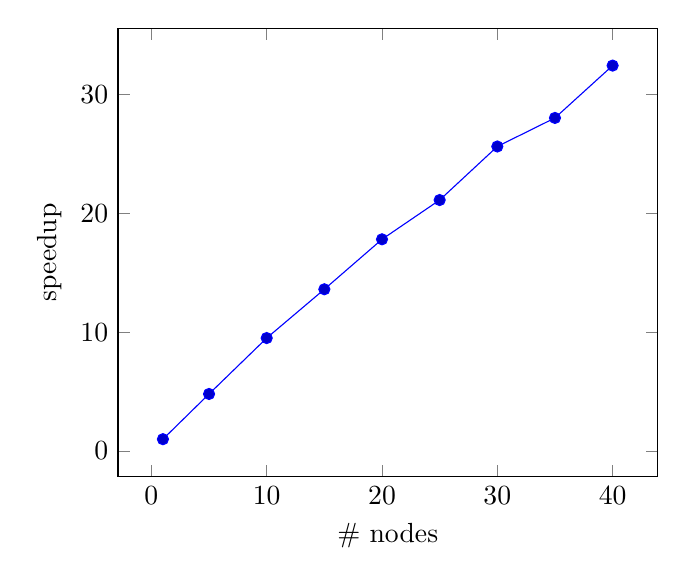
\begin{tikzpicture}
	\begin{axis}[xlabel=\# nodes,ylabel=speedup]
	\addplot coordinates {
		(1, 1)
		(5, 4.8)
		(10, 9.5)
		(15, 13.6)
		(20, 17.8)
		(25, 21.1)
		(30, 25.6)
		(35, 28.0)
		(40, 32.4)
	};
	\end{axis}
	\end{tikzpicture}
	\caption{Observed speedup when traversing the GIT fan with varying numbers of compute nodes.}
	\label{graph:traversal_speedup}
\end{figure}

\begin{figure}[t]
	\centering
	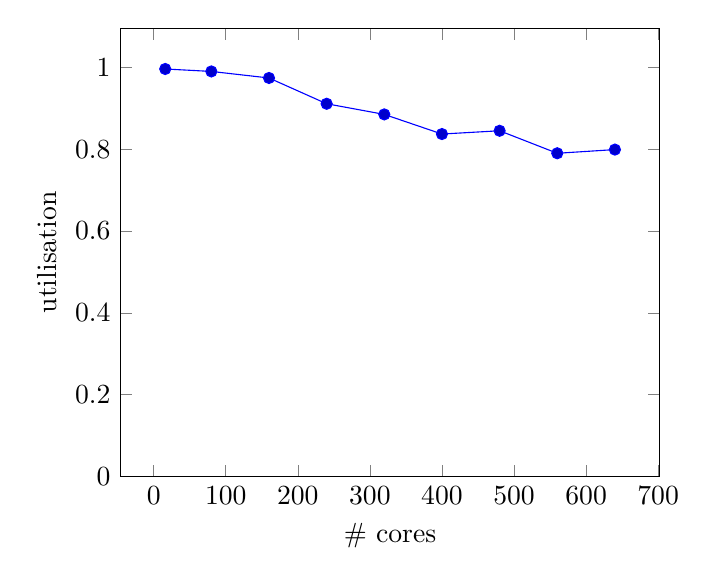
\begin{tikzpicture}
	\begin{axis}[xlabel=\# cores,ylabel=utilisation,ymin=0]
	\addplot coordinates {
		(16, 0.996)
		(80, 0.990)
		(160, 0.974)
		(240, 0.911)
		(320, 0.885)
		(400, 0.837)
		(480, 0.845)
		(560, 0.790)
		(640, 0.799)
	};
	\end{axis}
	\end{tikzpicture}
	\caption{Observed utilisation when traversing the GIT fan with varying numbers of compute nodes.}
	\label{graph:traversal_utilisation}
\end{figure}

\begin{figure}[t]
	\centering
	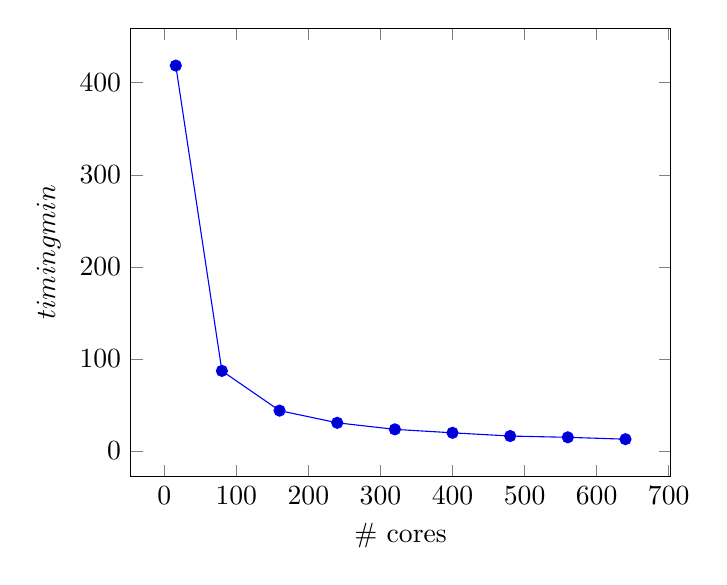
\begin{tikzpicture}
	\begin{axis}[xlabel=\# cores,ylabel=$\faktor{\text{timing}}{\text{min}}$]
	\addplot coordinates {
		(16, 418.5950)
		(80, 87.0672)
		(160, 43.9218)
		(240, 30.6985)
		(320, 23.5702)
		(400, 19.8228)
		(480, 16.3206)
		(560, 14.9239)
		(640, 12.9088)
	};
	\end{axis}
	\end{tikzpicture}
	\caption{Required computation time when traversing the GIT fan with varying numbers of compute nodes.}
	\label{graph:traversal_timing}
\end{figure}
	\chapter{Application: Moduli space of $n$\=/pointed stable curves}
\label{chapter:moduli_space_of_pointed_stable_curves}

In order to profile and test our implementation, we are going to compute the Mori chamber decomposition of the moduli space $\overline{M}_{0,n}$ of $n$\=/pointed stable curves of genus $0$ for $n=5,6$. Essentially, this is achieved by determining the GIT fan of a graded divisoral algebra, where the grading specifies the group action on its variety. This chapter is devoted to this specific application. First, we give a concise introduction of the moduli space $\overline{M}_{0,n}$. In the second section, we define Mori dream spaces and remark that $\overline{M}_{0,n}$ indeed is such a space. Finally, we present the notion of cones of divisors and Mori chamber decompositions by means of $\overline{M}_{0,n}$.

For the remainder of this chapter, fix $n\in\natural$.

\section{Moduli space of $n$\=/pointed stable curves of genus 0}

We consider the moduli space $M_{0,n}$ of $n$\=/pointed rational curves of genus $0$ up to isomorphism, that is $M_{0,n}$ consists of classes of (ordered) configurations $(C,p_1,\dots,p_n)$ with $C$ being a smooth, projective curve of genus $0$ and the $p_i$ are distinct, smooth points located on $C$. Two configurations $(C,p_1,\dots,p_n)$ and $(C',p_1',\dots,p_n')$ are said to be equivalent iff there exists an isomorphism $\varphi: C \longrightarrow C'$ such that $\varphi(p_i) = p_i'$ for all $1\leq i \leq n$.
\index{M0n@$M_{0,n}$}%

We give a concrete description of $M_{0,n}$. Each smooth, projective curve of genus $0$ is isomorphic to $\projective^1$ \cite[Example IV.1.3.5]{hartshorne}. For this reason any configuration in $M_{0,n}$ may be represented by $(\projective^1, p_1,\dots,p_n)$ with $p_i\in \projective^1$ and $p_i \neq p_j$ for $i\neq j$. It is well known that for any triplet $(q_1, q_2, q_3)$ of distinct points there exists exactly one automorphism of $\projective^1$ sending this triplet to $(0,1,\infty)$. By applying the automorphism sending the first three points of our configuration to $0$, $1$ and $\infty$ respectively, we obtain a unique representative $(\projective^1, 0, 1, \infty, p_4',\dots,p_n')$ such that $p_4'$ up to $p_n'$ are distinct points contained in $\projective^1\setminus\{0,1,\infty\}$. By going over to the affine chart $\projective^1\setminus\{\infty\}\cong \mathbb{A}^1$ of $\projective^1$, we conclude that

$$M_{0,n} \cong \{(p_1,\dots,p_{n-3})\in (\complex \setminus \{0,1\})^{n-3} \mid p_i\neq p_j\ \mathrm{for}\ i\neq j\}.$$

By alleviating the condition on the curve $C$, Deligne and Mumford were able to construct a compactification $\overline{M}_{0,n}$ that does not only parametrise $n$\=/pointed smooth curves, but also the following $n$\=/pointed stable curves. \cite{curves_of_a_given_genus}
\index{M0n2@$\overline{M}_{0,n}$}%

\begin{defi}[\phantom{}{\cite[section 1.2]{stable_npointed_curves}}]
	\label{defi:stable_npointed_curve}
	An \emph{$n$\=/pointed stable curve of genus $0$} is a configuration $(C,p_1,\dots,p_n)$ where $C$ is a connected, projective curve and the marked points $p_i\in C$ are distinct and smooth such that
	\begin{enumerate}[label={\upshape(\roman*)}]
		\item Every irreducible component of $C$ is isomorphic to $\projective^1$,
		\item Irreducible components intersect in nodal points. A nodal point is an ordinary double point that is passed by exactly two branches of $C$ with different tangent lines.
		\item If $\delta$ is the number of nodal points, there are $\delta + 1 $ irreducible components.
		\item Every irreducible component contains at least three of the marked or nodal points on $C$.
	\end{enumerate}
\end{defi}

\begin{remark}
	Note that all curves $C$ satisfying the conditions (i)-(iii) in Definition~\ref{defi:stable_npointed_curve} have arithmetic genus $0$. Furthermore, any automorphism of $C$ fixing all marked points is trivial, hence the name ``stable''. The set $M_{0,n}$ appears as open subset in $\overline{M}_{0,n}$ and corresponds to $n$\=/pointed stable curves which are smooth.
\end{remark}

\section{Divisors \& Cox rings \& Mori dream spaces}

We introduce the notions of Cox rings and Mori dream spaces, cones of divisors and chamber decompositions as in \cite{cox_rings}. They relate to $\overline{M}_{0,n}$ in the sense that $\overline{M}_{0,n}$ is a Mori dream space for which we compute the Mori chamber decomposition. Let $X$ be an irreducible, normal prevariety over an algebraically closed field $\field$ of characteristic zero.

\begin{defi}[Divisor]
	A \emph{prime divisor} of $X$ is an irreducible subvariety $D\subseteq X$ of codimension $1$. The free abelian group generated by all prime divisors of $X$ is called the \emph{divisor group} of $X$, denoted by $\Div(X)$. Its elements are called \emph{divisors}.
	\index{Div(X)@$\Div(X)$}%
	
	The \emph{support} of a divisor $D = z_1 D_1 + \dots + z_s D_s$ with prime divisors $D_i$ and integers $z_i$ is given by
	$$\Supp(D) \defeq \bigcup_{z_i \neq 0} D_i.$$
	\index{Supp(X)@$\Supp(X)$}%
	The divisor $D$is called \emph{effective}, denoted by $D \geq 0$, if $z_i \geq 0 $ for all $i$.
	\index{D>=0@$D \geq 0$}%
\end{defi}

Note, that for us, divisors are weil but not necessarily cartier.

Any prime divisor $D$ corresponds to a generic point $\eta_D$ of $X$. Since $X$ is normal, its local ring $\O_{X,\eta_D}$ becomes a discrete valuation ring with discrete valuation $\nu_D\colon K(X)^* \rightarrow \integer$. For this reason, any nonzero rational function $f\in K(X)^*$ defines a divisor as follows:

\begin{defi}
	Let $f\in K(X)^*$. Then we define
	$$\div(f) \defeq \sum_{D\ \text{prime}} \nu_D(f) \cdot D.$$
	Divisors of the form $\div(f)$ are called \emph{principal divisors}. The set of all principal divisors is denoted by $\PDiv(X)$.
	\index{div(f)@$\div(f)$}%
	\index{PDiv(X)@$\PDiv(X)$}%
\end{defi}

\begin{remark}
	The map $\div\colon K(X)^* \rightarrow \Div(X)$ is well defined and a group homomorphism. In particular, $\PDiv(X)$ is a subgroup of $\Div(X)$. The factor group
	$$\Cl(X) \defeq \faktor{\Div(X)}{\PDiv(X)}$$
	is called the \emph{divisor class group} of $X$.
	\index{Cl(X)@$\Cl(X)$}%
\end{remark}

\begin{defi}
	\label{defi:divisor_restriction}
	Let $U\subseteq X$ be open. We define the restriction map $\Div(X) \rightarrow \Div(U)$ by the $\integer$\=/linear extension of 
	$$D\restrict{U} \defeq \begin{cases}
	D\cap U, & D\cap U \neq \emptyset \\
	0,	& \text{else}
	\end{cases}$$
	for any prime divisor $D$ of $X$.
\end{defi}

\begin{defi}
	Let $D\in\Div(X)$. Then we define the sheaf $\O_X(D)$ of $\O_X$\=/modules as follows:
	$$\O_X(D)(U) \defeq \{f\in K(X)^*\mid (\div(f) + D)\restrict{U} \geq 0\} \cup \{0\}\quad \forall U\subseteq X\ \text{open}.$$
	The restriction map is given as in Definition~\ref{defi:divisor_restriction}. Note that we have 
	$$\O_X(D_1)(U)\cdot \O_X(D_2)(U) \subseteq \O_X(D_1 + D_2)(U)$$
	for any open subset $U\subseteq X$ and divisors $D_1,D_2\in\Div(X)$.
	\index{OXD@$\O_X(D)$}%
\end{defi}

\begin{defi}[Movable divisor]
	Let $D$ be a divisor of $X$. The \emph{base locus} of $D$ is defined by
	$$\text{Bs}\ |D| \defeq \bigcap_{f\in\O_X(D)(X)} \Supp(\div(f) + D)$$
	and the \emph{stable base locus} is
	$$\textbf{B}\ |D| \defeq \bigcap_{n\in\natural} \text{Bs}\ |nD|.$$
	We say that $D$ is \emph{movable} iff its stable base locus is of codimension at least $2$ in $X$, that is, it does not contain any prime divisors.
	\index{BsD@$\text{Bs}\ \vert D \vert$}%
	\index{BD@$\textbf{B}\ \vert D \vert$}%
\end{defi}

\begin{defi}[Cox ring]
	Let $X$ be such that its divisor class group $\Cl(X)$ is finitely generated and there exists a subgroup $K$ of $\Div(X)$ that is a representative system of the orbits of $\Div(X)$ w.r.t. $\PDiv(X)$. Then the \emph{Cox sheaf} of $X$ is the sheaf of divisoral algebras given by
	$$\mathcal{R} \defeq \bigoplus_{D\in K} \mathcal{R}_{[D]} = \bigoplus_{[D]\in \Cl(X)} \mathcal{R}_{[D]}, \quad\quad \mathcal{R}_{[D]} \defeq \O_X(D).$$
	Up to isomorphy, it does not depend on the choice of $K$. The \emph{Cox ring} of $X$ is the $\Cl(X)$\=/graded algebra of global sections $\mathcal{R}(X)$.
	\index{RX@$\mathcal{R}(X)$}%
\end{defi}

In the construction of Cox rings presented here, we do rely on the existence of a subgroup of $\Div(X)$ being a representative system. In general, it suffices to demand a subgroup of $\Div(X)$ such that the equivalence classes of its elements cover all $\Cl(X)$, see \cite[Construction 1.4.2.1]{cox_rings}.

\begin{defi}[Mori dream space]
	Let $X$ be an irreducible, normal projective variety. It is called a \emph{Mori dream space} if its divisor class group $\Cl(X)$ and its Cox ring $\mathcal{R}$ are finitely generated.
\end{defi}

\begin{remark}
	\label{remark:mn_setup}
	Whereas the Deligne\=/Mumford compactification $\overline{M}_{0,n}$ of the moduli space of $n$\=/pointed stable curves of genus $0$ is no Mori dream space for sufficiently large $n$ \cite{mn_is_not_a_mori_dream_space}, for $n=5,6$, its Cox ring is finitely generated. A set of homogenous generators of $\mathcal{R}(\overline{M}_{0,5})$ is identified by \cite{cox_ring_del_pezzo_surface} since $\overline{M}_{0,5}$ is a del Pezzo surface \cite{bernal}. In \cite{cox_ring_of_msix}, \citeauthor{cox_ring_of_msix} determines a set of homogenous generators for $\mathcal{R}(\overline{M}_{0,6})$. \citeauthor{bernal} \cite{bernal} then computes the relations between the generators so that a presentation of the Cox rings in terms of a zero locus is obtained. Furthermore, she provides an explicit description of the symmetry group action on $\mathcal{R}(\overline{M}_{0,5})$ and $\mathcal{R}(\overline{M}_{0,6})$ respectively that arises from permuting marked points in a configuration, that is 
	$$\sigma\cdot(C,p_1,\dots,p_n) \defeq (C,p_{\sigma(1)},\dots,p_{\sigma(n)})\quad \forall\sigma\in \mathcal{S}_n.$$
	
	Hence, we obtain embedding of the Cox ring as in \ref{construction:algebraic_torus}. The torus action is defined by the grading living in the divisor class group, which is a finitely generated subgroup of some $\integer^d$. This defines the matrix $Q$ in our setup of section~\ref{section:setup}. The vanishing ideal $\ideal$ is given by the relations between the generators. \citeauthor{bernal}'s description of the symmetry group action extends our setup in the sense of section~\ref{sec:exploiting_symmetry}.
\end{remark}

\section{Mori chamber decomposition}

In this section we refer to $\overline{M}_{0,n}$ as a Mori dream space and tacitly assume that $n=5$ or $n=6$. With Remark~\ref{remark:mn_setup} in mind, we see that the lattice points of the weight cone of $\mathcal{R}(\overline{M}_{0,n})$ as in section~\ref{sec:git_fan} are in fact divisor classes of $\overline{M}_{0,n}$. It lives in the ambient space $\Cl(\overline{M}_{0,n}) \tensor_\integer \rational$. For this reason, all cones arising in section~\ref{sec:git_fan} are considered to be cones of divisors classes such that its lattice points are elements in $\Cl(\overline{M}_{0,n})$. We are interested in two particular cones:

\begin{defi}
	The \emph{cone of effective [movable] divisor classes} of $\overline{M}_{0,n}$ is given by
	$$\Eff(\overline{M}_{0,n}) = \langle [D] \tensor 1 \mid D\in\Div(\overline{M}_{0,n})\ \text{effective} \rangle_{\rational{> 0}},$$
	$$\Mov(\overline{M}_{0,n}) = \langle [D] \tensor 1 \mid D\in\Div(\overline{M}_{0,n})\ \text{movable} \rangle_{\rational{> 0}}.$$
	\index{EffM0n@$\Eff(\overline{M}_{0,n})$}%
	\index{MovM0n@$\Mov(\overline{M}_{0,n})$}%
	
	Note that the sets of effective and movable divisors respectively are recovered by intersecting the above convex cones with $\Cl(\overline{M}_{0,n}) \tensor 1$. We also call the cone of movable divisor classes the \emph{moving cone}.
\end{defi}

\begin{remark}
	\label{remark:cone_of_divisor_classes_in_mn_context}
	By \cite[Proposition 3.3.2.1]{cox_rings}, the cone of effective divisor classes of $\overline{M}_{0,n}$ coincides with the weight cone of $\overline{M}_{0,n}$. Furthermore, in the setup of section~\ref{section:setup}, the moving cone is easily computed by intersecting all cones generated by all but one column of $Q$, that is
	$$\Mov(\overline{M}_{0,n}) = \bigcap_{\gamma_0 \preceq \gamma\ \mathrm{facet}} Q(\gamma_0)$$
	with the notation of chapter~\ref{chap:algorithm}. This claim is an immediate consequence of \cite[Proposition 3.3.2.3]{cox_rings}.
\end{remark}

\begin{defi}
	The \emph{Mori chamber decomposition} of the cone of effective divisor classes is the collection of chambers -- i.e. full dimensional cones -- of the GIT fan of $\overline{M}_{0,n}$. The \emph{Mori chamber decomposition} of the moving cone arises from the chambers of the fan obtained by intersecting the GIT fan with $\Mov(\overline{M}_{0,n})$.
\end{defi}

By \cite[Remark 3.3.4.2]{cox_rings}, the Mori chamber decomposition of the moving cone  $\Mov(\overline{M}_{0,n})$ parametrises all Mori dream spaces with Cox ring $\mathcal{R}(\overline{M}_{0,n})$ up to isomorphism. The implementation described in chapter~\ref{chap:implementation} allows us to compute the Mori chamber decompositions for $\Mov(\overline{M}_{0,n})$ efficiently. The input data for the algorithm is derived as in \ref{remark:mn_setup}. The explicit descriptions may be found in \cite{gitfan_symmetry}.

In order to speed up the computation of the Mori chamber decomposition of $\Mov(\overline{M}_{0,6})$, we dropped the generators of $\overline{M}_{0,6}$ corresponding to Keel-Vermeire divisors. Due to \cite[Remark 6.7]{gitfan_symmetry}, the Mori chamber decomposition of the moving cone is not altered by this modification. However, we reduce the problem size significantly, considering an embedding into $\field^{25}$ only instead of $\field^{40}$.

	\chapter{Conclusion}

In this thesis we presented a massively parallel approach for computing the GIT fan of a torus action on an affine variety. After explaining the mathematical background and the algorithmic idea of \citeauthor{gitfan_symmetry}, our realisation of the algorithm has been discussed in detail. \gpispace{} is the key component when it comes to developing an application that executes the GIT fan algorithm on large scale systems such as the cluster system of the \ac{Fraunhofer ITWM}. Concurrent parts have been reformulated in terms of Petri nets, whereas the sequential core operations are carried out by the computer algebra system \singular{}.

We have shown that the computation of the GIT fan translates to a graph traversal problem which is easily parallelised by expanding frontier nodes simultaneously. However, it is crucial that every computing node has a global view of the frontier set. Otherwise, nodes may be expanded several times, wasting potential computation time on the cluster system. For this reason we provided several storage implementations that manage a list of expanded nodes and frontier nodes. In our use case -- the computation of the Mori chamber decomposition of $\Mov(\overline{M}_{0,6})$ -- an in\=/memory solution on a single node, which is accessible via a RPC-server,  prevailed.

Our implementation scales almost linearly with the amount of available cores, obtaining a utilisation of still 80\% when using 640 cores. We were able to determine the Mori chamber representatives in approximately 21 minutes from a precomputed set of representatives for the faces of the simplex $\gamma$ under the $\mathcal{S}_6$\=/action. Previous implementations executed on a single machine with 16 cores terminated after a whole day. \cite[Rermark 6.8]{gitfan_symmetry}

In order to determine GIT fans with feasible effort, \citeauthor{gitfan_symmetry} introduced a fast monomial containment test and exploited symmetries occurring in the problem formulation. We contributed to this goal by optimising existing code and rewriting it for scalable hardware systems. However, some optimisations still are left open and may be revisited in future work. For one thing, we still rely on a precomputation by \gap{} that determines all representatives of the faces of $\gamma$. Although we provide a routine for this task, it does not utilise several cores and is too time\=/consuming when applied to the \msix{} example. Parallel implementations would be of high interest, increasing the scalability of our implementation further. Furthermore, our storage solution fails if the memory requirements -- given by the size of the GIT fan -- exceed the available RAM of a single node. The development of a distributed hash table with load balancing features would make the RAM of all nodes available such that scaling memory requirements may be satisfied without falling back to significant slower hard drives. This becomes particularly interesting in scenarios where cones cannot be encoded by short bit vectors of fixed length. Storing generating rays or defining half spaces requires an uncontrollable amount of memory due to exact representations of numbers in computer algebra systems.
	
	\appendix
	\chapter{Useful lemmata}

\begin{lemmaApp}
	\label{lemma:convex_fan_maximal_cones}
	Let $\Sigma\subseteq\mathbb{R}^k$ be a $k$-dimensional fan with convex support. Then $\Sigma$ is uniquely determined by $\Sigma^{(k)}$.
\end{lemmaApp}
\begin{proof}
	We show that every cone in $\Sigma$ is a face of a cone in $\Sigma^{(k)}$. Let $\tau\in\Sigma$ and choose a point $p\in\relint(\tau)$. We select hyperplanes $H_\theta$ for all $\theta\in\Sigma\setminus\Sigma^{(k)}$ such that $\theta\subseteq H_\theta$. Then we have
	$$S \defeq |\Sigma| \setminus \left(\bigcup_{\theta\in\Sigma\setminus\Sigma^{(k)}} H_\theta\right) \subseteq \bigcup_{\sigma\in\Sigma^{(k)}} \sigma \eqdef |\Sigma^{(k)}|.$$
	Since $|\Sigma|$ has dimension $k$ and $S$ arises from $|\Sigma|$ by removing finitely many hyperplanes, $S$ has dimension $k$. For this reason we find $q\in S \setminus\{p\}$. By Bézout's theorem, every hyperplane $H_\theta$ intersects the line through $p$ and $q$ in at most one point. As $|\Sigma|$ is convex, the connecting line $\overline{pq}$ is contained in $|\Sigma|$ and $\overline{pq} \cap S$ emerges from $\overline{pq}$ by removing a finite amount of points. Hence, we find a sequence $(p_n)_{n\in\natural}\subseteq \overline{pq} \cap S$ such that $\lim\limits_{n\rightarrow\infty} p_n = p$. It follows that $p\in\overline{S}$. Since $|\Sigma^{(k)}|$ is closed as a finite union of closed sets, $p\in|\Sigma^{(k)}|$ holds. Let $\sigma\in\Sigma^{(k)}$ such that $p\in\sigma$. Then the common face of $\sigma$ and $\tau$ contains $p$ and thus has to be $\tau$. We conclude that $\tau\preceq\sigma$.
\end{proof}

\chapter{Ideal quotients}
\label{appendix:ideal_quotients}

Theory about saturated ideals allows us to implement an efficient monomial containment test, see \cite{gitfan_symmetry}. Here, we establish some elementary properties that are used in this thesis.

\begin{defiApp}
	Let $I,J$ be ideals over a commutative ring $R$. Then we define the \emph{ideal quotient} $(I:J)$ by
	$$(I:J) = \{r\in R\ |\ rJ\subseteq I\}.$$
	The \emph{saturation} $(I:J^\infty)$ is given by
	$$(I:J^\infty) = \bigcup_{n\in \natural}(I:J^n).$$
\end{defiApp}

\begin{propApp}
	Let $I$, $J$, $K$ be ideals over $R$ and let $f,g\in R$. Then we have:
	\begin{enumerate}[label={\upshape(\roman*)}]
		\item $I\subseteq J\ \Rightarrow\ (I:K^\infty)\subseteq(J:K^\infty)$,
		\label{enum_item:saturation_inclusion_property}
		\item $((I:(f)^\infty):(g)^\infty) = (I:(fg)^\infty)$.
		\label{enum_item:saturation_principal_property}
	\end{enumerate}
\end{propApp}
\begin{proof}
	\ref{enum_item:saturation_inclusion_property} immediately follows from the definition. For \ref{enum_item:saturation_principal_property}, note that
	$$(I:(f)) = \{r\in R\ |\ rf\in I\}\quad\text{and}\quad (I:(f)^\infty) = \{r\in R\ |\ \exists n\in\natural: rf^n\in I\}.$$
	
	Let $r\in (I:(fg)^\infty)$. We find $n\in \natural$ such that $(rg^n)f^n = r(fg)^n\in I$. Hence, $rg^n\in (I:(f)^\infty)$. It follows that $r\in((I:(f)^\infty):(g)^\infty)$.
	
	Conversely, let $r\in((I:(f)^\infty):(g)^\infty)$. Then we find $n\in \natural$ such that $rg^n\in (I:(f)^\infty)$. This implies that there exists an $m\in\natural$ such that $rg^nf^m\in I$. For this reason $r(fg)^{\max\{n,m\}}\in I$ and thus $r\in (I:(fg)^\infty)$ holds, proving \ref{enum_item:saturation_principal_property}.
\end{proof}
	
	% Literaturhinweise
	\backmatter
	\nocite{*}
	\phantomsection
	\addcontentsline{toc}{chapter}{Bibliography}
	\printbibliography
	
	% Abkürzungsverzeichnis
	\chapter*{List of abbreviations}
\addcontentsline{toc}{chapter}{List of abbreviations}

\begin{acronym}[Fraunhofer ITWM]
	\acro{BLOB}{Binary Large Object}
	\acro{DRTS}{distributed run-time engine}
	\acro{Fraunhofer ITWM}{\emph{Fraunhofer-Institut für Techno- und Wirtschaftsmathematik}}
	\acro{GIT}{Geometric Invariant Theory}
	\acro{PGAS}{partitioned global address space}
	\acro{RIFD}{Remote Interface Daemon}
	\acro{ssi}{simple singular interface}
	\acro{STL}{Standard Template Library}
	\acro{WE}{workflow engine}
\end{acronym}
	
	% Index
	\cleardoublepage
	\phantomsection
	\addcontentsline{toc}{chapter}{Index}
	\printindex
	
	% Abkürzungsverzeichnis
	%\cleardoublepage
	%\addcontentsline{toc}{chapter}{List of abbreviations}
	%\input{includes/acronyms}
	
	% Selbstständigkeitserklärung
	\cleardoublepage
	{
		\pagestyle{empty}
		\vspace*{\fill}

\begin{flushright}
	\Huge Erklärung zu dieser Arbeit
\end{flushright}

\vspace{1cm}

Hiermit erkläre ich, die vorliegende Masterarbeit selbstständig erstellt zu haben. Weiterhin versichere ich, dass sämtliche von mir verwendeten Hilfsmittel und Quellen im Literaturverzeichnis aufgeführt sind.

\vspace{2cm}

\begin{flushright}
	$\overline{\parbox{10cm}{\hfill\textit{\Student, Hannover, den \AbgabeDerArbeit}}}$
\end{flushright}


	}
	
\end{document}
